\chapter{物理信息驱动的神经网络方法求解反势能问题}
\section{引言}
令 $\Omega\subseteq \bbR^{d}$ ($d\geq1$) 为一个具有光滑边界 $\partial\Omega$ 的有界连通区域。在本文中，我们考虑以下椭圆边值问题的势函数辨识
\begin{equation}\label{eq:pde:potential}
\left\{
\begin{aligned}
-\nabla\cdot(\alpha\nabla u)+qu&=f, \quad \text{在}~\Omega~\text{中},\\
\alpha\partial_{\nu}u&=g, \quad \text{在}~\partial\Omega~\text{上},
\end{aligned}
\right.
\end{equation}
其中给定了传导（或扩散）系数 $\alpha\in C^{1}(\bar{\Omega})$，源密度 $f\in L^{2}(\Omega)$ 和通量 $g\in L^{2}(\partial\Omega)$。空间依赖的势函数 $q$ 属于容许集
\begin{equation}\label{eq:box}
\calK=\{q\in L^{\infty}(\Omega):0\leq\underline{q}\leq q(x)\leq\overline{q}<\infty,~x\in\Omega\}.
\end{equation}
这里常数 $\underline{q}$ 和 $\overline{q}$ 分别代表容许势函数 $q(x)$ 的下界和上界。方程 \eqref{eq:pde:potential} 可以被视为与时间无关的 Schr{\"o}dinger 方程 \cite{Bal2010Inverse}，其中 $q$ 是势函数。它还描述了扩散和热传递中的现象。具体而言，在与时间无关的扩散方程 \cite{Bal2010Inverse} 中，$q$ 对应于吸收（或反应）系数，而在稳态热方程中，$q$ 代表辐射系数~\cite{Chen2020Convergence}。
\par 实际上，系统方程 \eqref{eq:pde:potential} 中的势函数 $q$ 通常是未知的，目标是从整个区域 $\Omega$ 及其边界 $\partial\Omega$ 上 $u$ 的含噪测量值中恢复它。给定 $q\in\calK$，方程 \eqref{eq:pde:potential} 存在唯一解 $u_{q}\in H^{1}(\Omega)$ \cite{evans2010partial}。我们因此可以定义一个正演算子 $\calF:q\mapsto u_{q}$。在整篇文章中，假设含噪测量数据是由以下标准高斯回归模型生成的
\begin{equation}\label{eq:measurement}
\left\{
\begin{array}{rcll}
z^{\delta}(x)&=&\calF(q^{\dagger})(x)+\varepsilon_{\calI}(x),\quad &\varepsilon_{\calI}(x)\sim N(0,\delta^{2}),\quad x\in\Omega, \\ 
Tz^{\delta}(x)&=&T\calF(q^{\dagger})(x)+\varepsilon_{\calB}(x),\quad &\varepsilon_{\calB}(x)\sim N(0,\delta^{2}),\quad x\in\partial\Omega,
\end{array}
\right.
\end{equation}
其中 $q^\dagger$ 代表真实的势函数，$\delta$ 表示正的噪声水平，$T$ 是迹算子。很容易验证 $\|z^{\delta}-\calF(q^{\dagger})\|_{L^{2}(\Omega)}=|\Omega|^{1/2}\delta$ 且 $\|Tz^{\delta}-T\calF(q^{\dagger})\|_{L^{2}(\partial\Omega)}=|\partial\Omega|^{1/2}\delta$。

在本文中，我们提出了 Tikhonov-PINNs，一种基于神经网络的求解反势问题的方法。该方法背后的核心概念是将 Tikhonov 正则化与 PINNs 相结合。与~\cite{duan2024recovering} 不同，我们像 \cite{jin2024stochastic} 中那样，为非线性势识别问题的随机收敛性建立了误差估计，将适用范围扩展到了线性场景和有界噪声考量之外。综上所述，我们的主要贡献列举如下：

\begin{itemize}
\item[(i)] 我们提出了 Tikhonov-PINNs，这是一种通过整合 Tikhonov 正则化和 PINNs 来求解反势问题的无网格数值重构算法。通过这种整合，我们为反势问题引入了新的稳定性估计，建立了物理信息损失误差与重构收敛率之间的联系。

\item[(ii)] 我们进行了一系列数值实验来展示 Tikhonov-PINNs 的有效性。通过将其应用于不同噪声水平测量下的光滑和不连续势函数，我们要证明所提出的方法在精度和鲁棒性方面均优于经典的基于有限元的方法以及原始 PINNs。

\item[(iii)] 我们给出了 Tikhonov-PINNs 的系统性收敛分析。我们的理论结果表明，在合适的神经网络参数和 $u$ 的一些正性条件下，重构解 $\hat{q}$ 表现出如下趋向于真实值 $q^{\dagger}$ 的收敛行为：
\[
\mathbb{E}_{\calS}\left[\|\hat{q}-q^\dagger\|_{L^2(\Omega)}\right] \leq \mathcal{O}\left(\delta^{\frac{1}{2(1+2\beta)}}\cdot\max\left\{ \log\left( \frac{1}{\delta} \right), 1 \right\}\right).
\]
期望 $\mathbb{E}_{\calS}$ 是在随机样本 $\calS$ 上选取的，$\beta>0$ 为常数。详情请参见定理 \ref{thm:excess} 和定理 \ref{thm:ConvergenceRate}。进一步的分析表明，我们的方法部分克服了维数灾难 (CoD)。
\end{itemize}

本文的其余部分组织如下。在第 \ref{prelim} 节中，我们介绍了预备知识和符号说明。针对反势问题的重构方法，即 Tikhonov-PINNs，随后在第 \ref{sec:tikpinns} 节中进行介绍。误差分析结果在第 \ref{sec:erroranalysis} 节中陈述，其证明包含在第 \ref{sec:proof} 节中。在第 \ref{sec:numerical} 节中，我们提供了一些数值算例以展示我们方法的有效性。最后，我们在第 \ref{sec:conclusion} 节中给出结论并进行进一步讨论。



\section{预备知识与符号说明}\label{prelim}




\section{重构方法：Tikhonov-PINNs}\label{sec:tikpinns}
\par 给定 Eq.\eqref{eq:measurement} 中的测量数据，我们利用 $H^2$ 范数惩罚项来重构 $q$：

\begin{equation*}
\min_{q\in\calK}\Big\{J_{\lambda}(q)=\|z^{\delta}-\calF(q)\|_{L^{2}(\Omega)}^{2}+\|Tz^{\delta}-T\calF(q)\|_{L^{2}(\partial\Omega)}^{2}+\lambda\|q\|_{H^{2}(\Omega)}^{2}\Big\},
\end{equation*}
这等价于一个线性二次椭圆控制问题
\begin{align*}
&\min_{q,u}\quad\calJ_{\lambda}(q,u)=\|z^{\delta}-u\|_{L^{2}(\Omega)}^{2}+\|Tz^{\delta}-Tu\|_{L^{2}(\partial\Omega)}^{2}+\lambda\|q\|_{H^{2}(\Omega)}^{2}, \\
&\subto\quad Eq.\eqref{eq:pde:potential}~\text{and}~Eq.\eqref{eq:box}.
\end{align*}
处理上述 PDE 约束优化问题的一个自然方法是引入物理信息惩罚项，将其转化为无约束问题
\begin{equation}\label{eq:pinns:loss}
\min_{q,u}\Big\{\calL_{\lambda}(q,u)=\calJ_{\lambda}(q,u)+\calI(q,u)+\calB(q,u)\Big\},
\end{equation}
其中
\begin{equation*}
\calI(q,u)=\|\nabla\cdot(\alpha\nabla u)-qu+f\|_{L^{2}(\Omega)}^{2}\quad\text{and}\quad
\calB(u)=\|\alpha\partial_{\nu}u-g\|_{L^{2}(\partial\Omega)}^{2}.
\end{equation*}
与传统 PINNs 不同，我们在损失函数中引入了一个额外的 Tikhonov 正则化项。正如我们将在下文中证明的，这一调整确保了重构势函数 $q$ 的收敛性。这在文献中通常被称为稳定性估计。为了推导这一结果，我们对 $q$ 和 $u$ 施加如下正则性假设。
\begin{assumption}\label{ass:potential:qudaggerreg}
令 $s \in \mathbb{N}_+$，我们假设 $q^\dagger \in W^{2,\infty}(\Omega) \cap H^{s+3}(\Omega) \cap K$ 且 $u^\dagger \in W^{2,\infty}(\Omega) \cap H^{s+3}(\Omega)$。
\end{assumption}
\begin{theorem}[稳定性估计]\label{th:potential:stability}
在 Eq.\eqref{eq:pde:potential} 和 Eq.\eqref{eq:measurement} 的模型下。令 $(q^{\dagger},u^{\dagger})$ 满足 Eq.\eqref{eq:pde:potential}。假设 Assumption \ref{ass:potential:qudaggerreg} 成立，则对于每一对满足 $q\in H^{2}(\Omega)$ 的 $(q,u)$，有
\begin{equation*}
\|(q-q^{\dagger})u^{\dagger}\|_{L^{2}(\Omega)}\leq C(1+\lambda^{-1/4}\calL_{\lambda}^{1/4}(q,u))(\calL_{\lambda}^{1/4}(q,u)+\delta^{1/2}),
\end{equation*}
其中 $C$ 是一个依赖于 $d$, $\Omega$, $\alpha$, $\overline{q}$, $\|q^{\dagger}\|_{W^{2,\infty}(\Omega)}$ 和 $\|u^{\dagger}\|_{W^{2,\infty}(\Omega)}$ 的正常数。
\end{theorem}
\begin{proof}
详细证明见 \ref{sec:lemma4} 小节。
\end{proof}
\par 在实际应用中，只能获得由 Eq.\eqref{eq:measurement} 生成的有限测量数据。令 $\euD_{\calI}=\{(x_{i},z_{i}^{\delta})\}_{i=1}^{m_{\calI}}$ 和 $\euD_{\calB}=\{(\bar{x}_{i},Tz_{i}^{\delta})\}_{i=1}^{m_{\calB}}$ 为测量数据集，其中 $\{x_{i}\}_{i=1}^{m_{\calI}}\subseteq\Omega$, $\{\bar{x}_{i}\}_{i=1}^{m_{\calB}}\subseteq\partial\Omega$, $z_{i}^{\delta}=z^{\delta}(x_{i})$ 且 $\bar{z}_{i}^{\delta}=Tz^{\delta}(\bar{x}_{i})$。假设 $\euX_{\calI}=\{x_{j}^{\calI}\}_{j=1}^{n_{\calI}}$ 和 $\euX_{\calB}=\{x_{j}^{\calB}\}_{j=1}^{n_{\calB}}$ 是分别从 $\Omega$ 和 $\partial\Omega$ 上的均匀分布中独立同分布抽取的两组点集。
通过将测量数据集代入目标泛函并使用蒙特卡洛方法离散化积分，我们可以获得如下经验损失函数
\begin{equation}\label{eq:empirical:loss}
\what{\calL}_{\lambda}(q,u)=\what{\calJ}_{\lambda}(q,u)+\what{\calI}(q,u)+\what{\calB}(u),
\end{equation}
该函数以数据集 $\euD_{\calI}$，$\euD_{\calB}$，$\euX_{\calI}$ 和 $\euX_{\calB}$ 为条件。其中
\begin{align*}
\what{\calJ}_{\lambda}(q,u)&=\|z^{\delta}-u\|_{L^{2}(\euD_{\calI})}^{2}+\|Tz^{\delta}-Tu\|_{L^{2}(\euD_{\calB})}^{2}+\lambda\|q\|_{H^{2}(\euX_{\calI})}^{2} \\
&=\frac{|\Omega|}{m_{\calI}}\sum_{i=1}^{m_{\calI}}(z_{i}^{\delta}-u(x_{i}))^{2}+\frac{|\partial\Omega|}{m_{\calB}}\sum_{i=1}^{m_{\calB}}(\bar{z}_{i}^{\delta}-Tu(\bar{x}_{i}))^{2} \\
&\quad+\lambda\frac{|\Omega|}{n_{\calI}}\sum_{j=1}^{n_{\calI}}\Big\{q(x_{j}^{\calI})^{2}+\sum_{k=1}^{d}\partial_{k}q(x_{j}^{\calI})^{2}+\sum_{k=1}^{d}\sum_{\ell=1}^{d}\partial_{k}\partial_{\ell}q(x_{j}^{\calI})^{2}\Big\}, \\
\what{\calI}(q,u)&=\|\nabla\cdot(\alpha\nabla u)-qu+f\|_{L^{2}(\euX_{\calI})}^{2} \\
&=\frac{|\Omega|}{n_{\calI}}\sum_{j=1}^{n_{\calI}}(\nabla\cdot(\alpha(x_{j}^{\calI})\nabla u(x_{j}^{\calI}))-q(x_{j}^{\calI})u(x_{j}^{\calI})+f(x_{j}^{\calI}))^{2}, \\
\what{\calB}(u)&=\|\alpha\partial_{\nu}u-g\|_{L^{2}(\euX_{\calB})}^{2}=\frac{|\partial\Omega|}{n_{\calB}}\sum_{i=1}^{n_{\calB}}(\alpha(x_{j}^{\calB})\partial_{\nu}u(x_{j}^{\calB})-g(x_{j}^{\calB}))^{2}.
\end{align*}
随后数值解被定义为在某些神经网络类 $\calQ\times\calU$ 上最小化 Eq.\eqref{eq:empirical:loss}
\begin{equation}\label{eq:erm}
(\hat{q},\hat{u})\in\argmin_{(q,u)\in\calQ\times\calU}\what{\calL}_{\lambda}(q,u).
\end{equation}
在统计学术语中，Eq.\eqref{eq:erm} 被视为经验风险最小化，这等价于参数空间上的一个优化问题
\begin{equation*}
(\hat{\theta}_{q},\hat{\theta}_{u})\in\argmin_{(\theta_{q},\theta_{u})\in\Theta_{q}\times\Theta_{u}}\what{\calL}_{\lambda}(q(\theta_{q}),u(\theta_{u})).
\end{equation*}
详细的重构过程如算法 \ref{alg:TikPINNs} 所示。
\par\noindent
\begin{minipage}{\textwidth}
\renewcommand*\footnoterule{}
\renewcommand{\thempfootnote}{\fnsymbol{mpfootnote}}
\begin{algorithm}[H]
\caption{Tikhonov-PINNs}
\label{alg:TikPINNs}
\begin{algorithmic}[1]
\Require 数据集 $\euD_{\calI}$, $\euD_{\calB}$, $\euX_{\calI}$ 和 $\euX_{\calB}$。
\State 构建由 $(\theta_{q},\theta_{u})$ 参数化的神经网络 $(q(\theta_{q}),u(\theta_{u}))$。
\State 初始化参数 $(\theta_{q},\theta_{u})$。
\State \textcolor{white!30!black}{\texttt{\# Tikhonov-PINNs 训练。}}
\State \textcolor{white!30!black}{\texttt{\# 通过 Tikhonov-PINNs 损失估计 $(q(\theta_{q}),u(\theta_{u}))$。}}
\For {$k=1:\texttt{epochs}$}
\State {计算由 Eq.\eqref{eq:empirical:loss} 定义的经验 Tikhonov-PINNs 损失
\begin{equation*}
\what{\calL}_{\lambda}(q(\theta_{q}),u(\theta_{u}))=\what{\calJ}_{\lambda}(q(\theta_{q}),u(\theta_{u}))+\what{\calI}(q(\theta_{q}),u(\theta_{u}))+\what{\calB}(u(\theta_{u})).
\end{equation*}}
\State {反向传播 $(g_{\theta_{q}},g_{\theta_{u}})=\nabla\what{\calL}(q(\theta_{q}),u(\theta_{u}))$。}
\State {通过 SGD 类算法更新 $(\theta_{q},\theta_{u})$：$(\theta_{q},\theta_{u})\leftarrow\operatorname{SGD}\big\{(\theta_{q},\theta_{u}),(g_{\theta_{q}},g_{\theta_{u}}),\tau\big\}$。}
\EndFor
\Ensure {$(\hat{q},\hat{u})\leftarrow(q(\theta_{q}),u(\theta_{u}))$.}
\end{algorithmic}
\end{algorithm}
\end{minipage}
\begin{remark}
通过选择合适的激活函数，可以确保 $\calQ\subseteq H^{2}(\Omega)$。因此，Eqs.\eqref{eq:pinns:loss}\eqref{eq:empirical:loss} 中的 $H^{2}$-范数惩罚项是良定的，并且在理论上是合理的。
\end{remark}



\section{误差分析}\label{sec:erroranalysis}
\par 在本节中，我们将首先对超额风险（见 Eq.\eqref{eq:excessrisk0}）进行误差分析，深度学习理论文献 \cite{Johannes2020Nonparametric,Shen2022approximation} 对此投入了大量的数学研究工作。然后，通过将超额风险的误差界与稳定性估计相结合，获得势函数重构的收敛率。为简单起见，我们假设 $\|\alpha\|_{C^{1}(\bar\Omega)}\leq B_{\alpha}$，$\|f\|_{L^{\infty}(\Omega)}\leq B_{f}$ 以及 $\|g\|_{L^{\infty}(\partial\Omega)}\leq B_{g}$。在本节以及第~\ref{sec:proof} 节的详细证明中，我们采用以下关于网络架构和样本复杂度的假设。

\begin{assumption}\label{allcondition}
令 $s\in\bbN_{+}$ 和 $\mu>0$ 为任意给定常数（在引理 \ref{lemma:app:tanh} 中引入）。我们选择如下的网络和样本复杂度：
\begin{enumerate}
\item[(i)] 令 $\varrho = \tanh$。设置 $Q = N_\varrho(L_\calQ, S_\calQ, R_\calQ)$ 和 $\mathcal{U} = N_\varrho(L_\mathcal{\calU}, S_\mathcal{\calU}, R_\mathcal{\calU})$，使得
\[
L_\calQ = c\log(d + 2), \quad S_\calQ = C \cdot \varepsilon^{-\frac{d}{s+1-\mu}}, \quad R_\calQ = C \cdot \varepsilon^{-\frac{9d+4+4\mu}{2(s+1-\mu)} - 2},
\]   
\[
L_\mathcal{\calU} = c\log(d + 2), \quad S_\mathcal{\calU} = C \cdot \varepsilon^{-\frac{d}{s+1-\mu}}, \quad R_\mathcal{\calU} = C \cdot \varepsilon^{-\frac{9d+4+4\mu}{2(s+1-\mu)} - 2}.
\]
这里 $c$ 和 $C$ 是依赖于 $s$、$\Omega$ 和 $\mu$ 的常数，而 $C$ 还依赖于 $d$。
\item[(ii)] 令 $S = \{D_I, D_B, X_I, X_B\}$ 为数据集的集合，并且数据集大小由下式给出：
\[
\mathcal{O}(m_I) = \mathcal{O}(m_B) = \mathcal{O}(n_I) = \mathcal{O}(n_B)
\]    
\[
= C\left(\|q^\dagger\|_{H^{s+3}(\Omega)}^{-2} + \|u^\dagger\|_{H^{s+3}(\Omega)}^{-2}\right) \cdot \varepsilon^{-\frac{45d+16s+32}{s+1-\mu}c\log(d+2)-2}.
\]    
\item[(iii)] 令 $(\hat{q}, \hat{u}) \in Q \times \mathcal{U}$ 为由 \eqref{eq:erm} 给出的经验风险最小化器，它依赖于 $S$。
\end{enumerate}
\end{assumption}


%Furthermore, using the definition of $(q^{\dagger},u^{\dagger})$, we get 
%\begin{equation}
%\calL_{\lambda}(q,u)\leq\|u-u^{\dagger}\|_{L^{2}(\Omega)}^{2}+\|Tu-Tu^{\dagger}\|_{L^{2}(\partial\Omega)}^{2}+\calI(q,u)+\calB(u)+\lambda\|q\|_{H^{2}(\Omega)}^{2}.
%\end{equation}
正如我们将在 \ref{sec:lemma5} 小节中展示的那样，$\calE_{\lambda}(q,u)$ 可以分解为逼近误差和泛化误差。逼近误差代表了假设类 $\mathcal{Q} \times \mathcal{U}$ 上超额风险的下确界，并刻画了该类中函数的表达能力。另一方面，泛化误差衡量了由蒙特卡洛离散化引起的差异（即总体风险与其经验对应项之间的差距）。基于神经网络的逼近理论和学习理论，我们可以证明，通过恰当地选择网络和样本复杂度，可以在这两个误差之间实现权衡，从而得出以下关于超额风险的收敛结果。

%For the As stated in Lem. \ref{lemma:approximation}, the approximation error can be made arbitrarily small, provided that functions in the hypothesis class can approximate the target functions with sufficiently small error.
%
%As shown in the proof of Lem. \ref{lemma:errdec}, the generalization error increases as the metric entropy of the hypothesis classes becomes larger and converges to zero at a rate of $\calO(1/n)$ as the number of samples $n$ increases.
%
%The approximation and generalization errors both depend on the network parameters $L$, $S$, and $R$, but exhibit opposite trends. Thus, the sample sizes should be chosen to be sufficiently large to ensure that the generalization error converges to zero. By properly choosing the hyperparameters, a trade-off between the approximation and generalization errors can be achieved, leading to the following convergence result for the excess risk.

\begin{theorem}[超额风险界]\label{thm:excess}
在模型 Eq.\eqref{eq:pde:potential} 和 Eq.\eqref{eq:measurement} 下。令 $\varepsilon \in (0, 1)$ 并记 $\delta \in (0, 1)$ 为噪声水平。假设假设 \ref{ass:potential:qudaggerreg} 成立，如果我们按照假设 \ref{allcondition} 选择网络和样本复杂度，则我们有
$$
\mathbb{E}_S[\mathcal{E}_\lambda(\hat{q}, \hat{u})] \leq C\left(\|q^\dagger\|_{H^{s+3}(\Omega)}^{2} + \|u^\dagger\|_{H^{s+3}(\Omega)}^{2}\right) \cdot \varepsilon^2 \log(\frac{1}{\varepsilon}) + C\left(\|q^\dagger\|_{H^2(\Omega)}^{2} + 1\right) \cdot \lambda.
$$
这里 $C$ 是一个依赖于 $d$, $\Omega$, $s$, $B_\alpha$, $B_f$, $B_g$, $\overline{q}$, $q^\dagger$ 和 $u^\dagger$ 的正常数。
\end{theorem}
\begin{proof}
详细证明请参见 \ref{sec:excessrisk} 小节。
\end{proof}


% \subsection{收敛率}
% 我们现在展示本文的主要定理。正如该定理所揭示的，在适当的参数选择下，随着噪声水平的降低，Tikhonov-PINNs 对 $q$ 和 $u$ 的重构误差会收敛到零。

% \begin{theorem}[Tikhonov-PINNs 的收敛率] \label{thm:ConvergenceRate}
% 在模型 Eq.\eqref{eq:pde:potential} 和 Eq.\eqref{eq:measurement} 下。令 $\delta \in (0,1)$ 为噪声水平。假定假设 \ref{ass:potential:qudaggerreg} 成立，如果我们选择 $\varepsilon = O(\delta)$, $\lambda = O(\delta^2)$ 并按照假设 \ref{allcondition} 选择网络和样本复杂度，那么我们有

% \begin{align*}
% \max\left\{ \mathbb{E}_\calS \left\lVert \hat{u}-u^{\dagger} \right\rVert_{L^{2}(\Omega)}, \mathbb{E}_\calS \left\lVert T\hat{u}-Tu^{\dagger} \right\rVert_{L^{2}(\partial\Omega)} \right\} &\leq C \cdot \delta \cdot\max\left\{ \log\left( \frac{1}{\delta} \right), 1 \right\},\\
% \mathbb{E}_\calS \left\lVert (\hat{q}-q^{\dagger})u^{\dagger} \right\rVert_{L^{2}(\Omega)} &\leq C \cdot \delta^{1/2} \cdot\max\left\{ \log\left( \frac{1}{\delta} \right), 1 \right\}.
% \end{align*}
% 此外，如果存在某个 $\beta \geq 0$ 和 $\zeta > 0$ 使得 $u^{\dagger}(x) \geq \zeta \text{ dist}(x,\partial\Omega)^{\beta}$ 在 $\Omega$ 中几乎处处成立，则
% \[
% \mathbb{E}_\calS \left\lVert \hat{q}-q^{\dagger} \right\rVert_{L^{2}(\Omega)} \leq C' \cdot \delta^{\frac{1}{2(1 + 2\beta)}} \cdot\max\left\{ \log\left( \frac{1}{\delta} \right), 1 \right\}.
% \]
% 这里 $C,C'$ 是依赖于 $d$, $\Omega$, $s$, $B_{\alpha}$, $B_{f}$, $B_{g}$, $\overline{q}$, $q^{\dagger}$, $u^{\dagger}$ 的正常数，且 $C'$ 还依赖于 $\zeta$。
% \end{theorem}

% \begin{proof}
% 这是一个结合了稳定性估计（定理 \ref{th:potential:stability}）和超额风险界（定理 \ref{thm:excess}）的直接结果。详细证明请参见 \ref{sec:convergence} 小节。
% \end{proof}

% \begin{remark}[正性条件]
%       正性条件 $u^{\dagger}(x) \geq \zeta \text{ dist}(x,\partial\Omega)^{\beta}$ 量化了解 $u^{\dagger}$ 当 $\text{dist}(x,\partial\Omega) \to 0^{+}$ 时趋于零的衰减率。
% \end{remark}

% \begin{remark}[超参数选择]
% 根据定理 \ref{thm:ConvergenceRate}，通过按照假设 4.1 中概述的方式选择神经网络和样本复杂度，可以很好地控制重构误差。然而在实际应用中，优化误差和当前分析的非最优性质可能导致基于假设 4.1 直接计算参数变得不切实际。尽管如此，如下所示，增加网络宽度和样本量可以降低重构误差。
% \end{remark}

% \begin{remark}[缓解维数灾难]
% 值得注意的是，样本集的大小和神经网络的规模都以 $O(\delta^{-cd/s})$ 的速率增加，其中 $c > 0$ 为绝对常数。这意味着如果真实值 $(q^{\dagger},u^{\dagger})$ 具有足够的平滑度，维数灾难可以得到缓解。
% \end{remark}


% \section{数值实验}\label{sec:numerical}
% 在本节中，我们提供了几个例子来说明 Tikhonov-PINNs 的效率。首先，我们概述数值设置如下。

% \subsection{实验设置}
% 在训练 Tikhonov-PINNs 时，我们分别采用两个神经网络来逼近未知解 $u$ 和势函数 $q$。每个网络都是具有 $tanh$ 激活函数和每两层之间存在残差连接的 DNN。对于所有算例，我们进行了多次运行以确保结果的可靠性，并且为每种情况提供了详细的训练设置。

% 在接下来的小节中，我们将本文提出的方法与传统的基于有限元的方法进行了比较。具体而言，我们使用了开源库 \textbf{dolfin-adjoint} \cite{mitusch2019dolfin}，该库基于 \textbf{FEniCS} \cite{alnaes2015fenics,grossmann2024can} 构建，专为求解反问题和最优控制问题而设计。该库获得了 2015 年威尔金森数值软件奖 (Wilkinson Prize for Numerical Software)，并在科学界获得了广泛的认可和采用。

% 所有数值实验均在武汉大学超算集群上进行，使用 Python 3.12.3 实现。该超算系统配备了 128GB ECC 2400MHz DDR4 内存、Intel Xeon E5-2640v4 2.4GHz CPU 和 NVIDIA Tesla V100 16GB GPU。

% 我们已在 GitHub 上发布了所有训练代码，网址为 \url{https://github.com/shiki442/Tikhonov-PINNs}。该仓库包含完整的数据生成、训练和评估流程，以及每个算例的参考配置文件，以便于读者复现和进一步探索。

% \subsection{评估}
% 为了衡量重构势函数 $\hat{q}$ 和解 $\hat{u}$ 的精度，我们采用如下定义的相对 $L^{2}$ 误差：
% \begin{equation*}
% \err(\hat{q})=\frac{\|\hat{q}-q^{\dagger}\|_{L^{2}(\Omega)}}{\|q^{\dagger}\|_{L^{2}(\Omega)}}\quad\text{and}\quad\err(\hat{u})=\frac{\|\hat{u}-u^{\dagger}\|_{L^{2}(\Omega)}}{\|u^{\dagger}\|_{L^{2}(\Omega)}},
% \end{equation*}
% 这里，$L^2$ 范数是基于网格点上的值进行近似的，即 $\|v\|_{L^{2}(\Omega)}\approx\sqrt{\frac{1}{N}\sum_{i=1}^{N}v(x_{i})^{2}}$，其中 $\{x_{i}\}_{i=1}^{N}$ 为网格点。

% \subsection{光滑势问题}

% 在本小节中，我们利用光滑算例进行定量分析。为了最小化优化误差的影响，我们使用充足的样本数量将网络训练了足够长的时间。

% \subsubsection{一维问题}
% \begin{figure}[htbp]
%     \centering
%     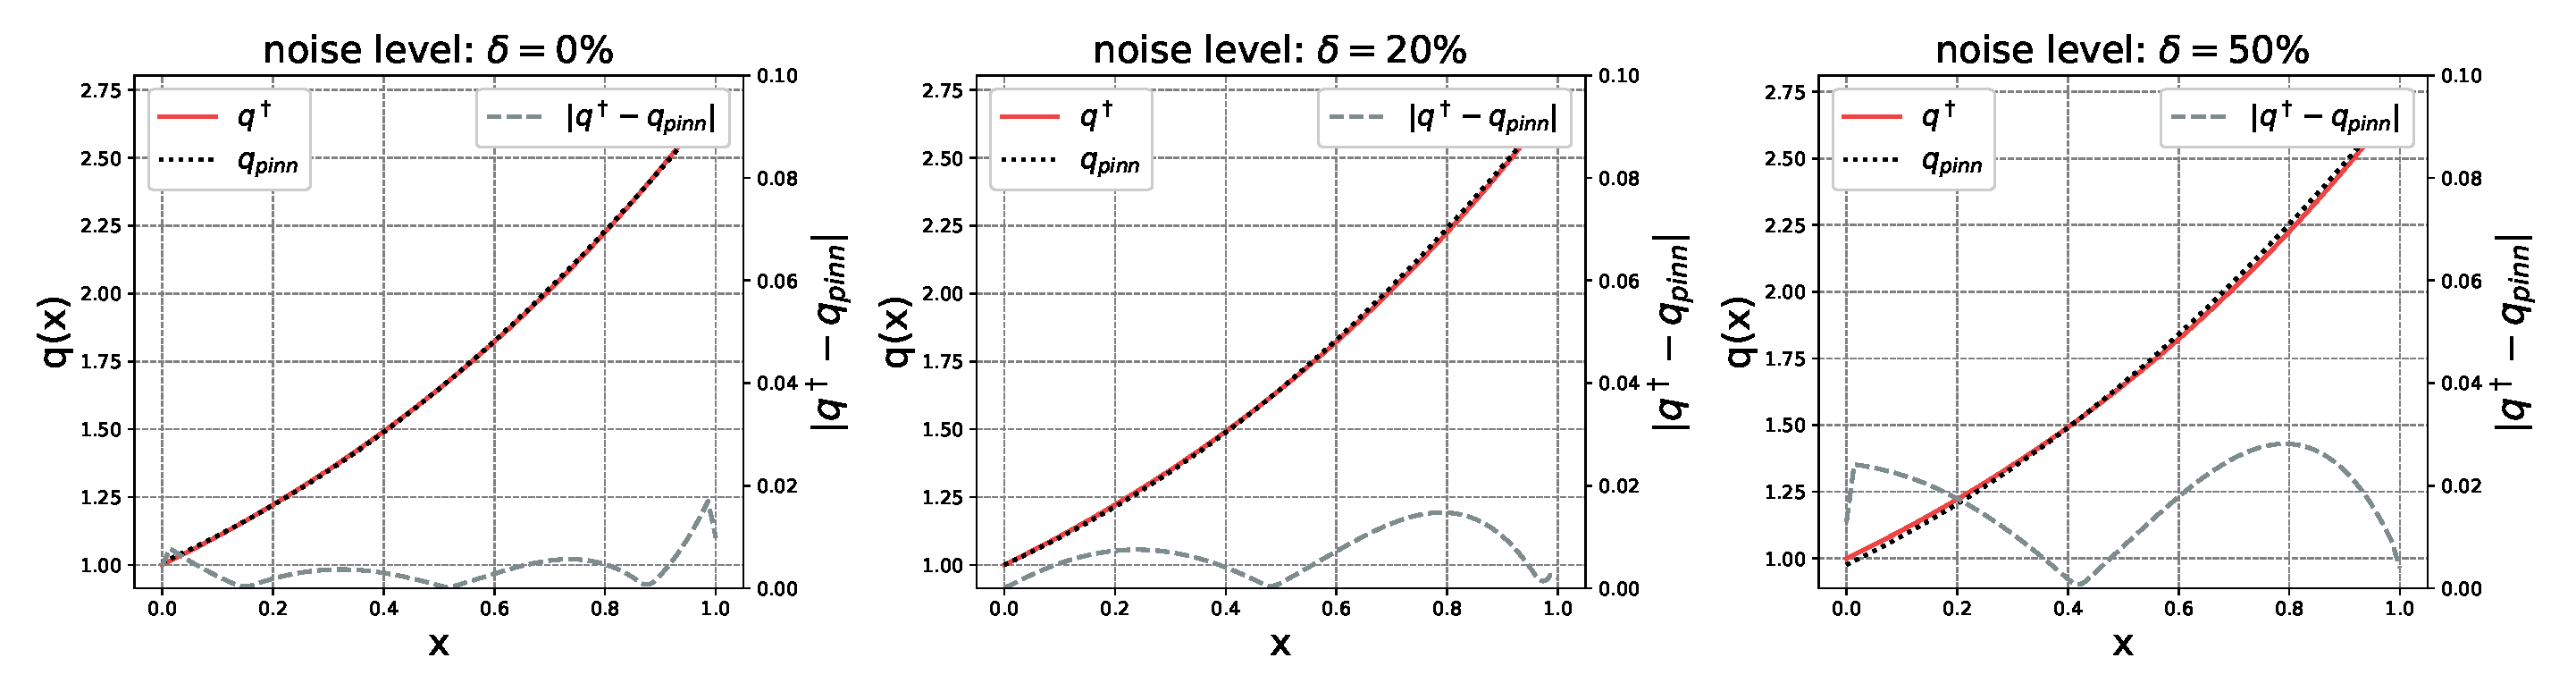
\includegraphics[width=\textwidth]{figures3/ex0_q.eps}
%     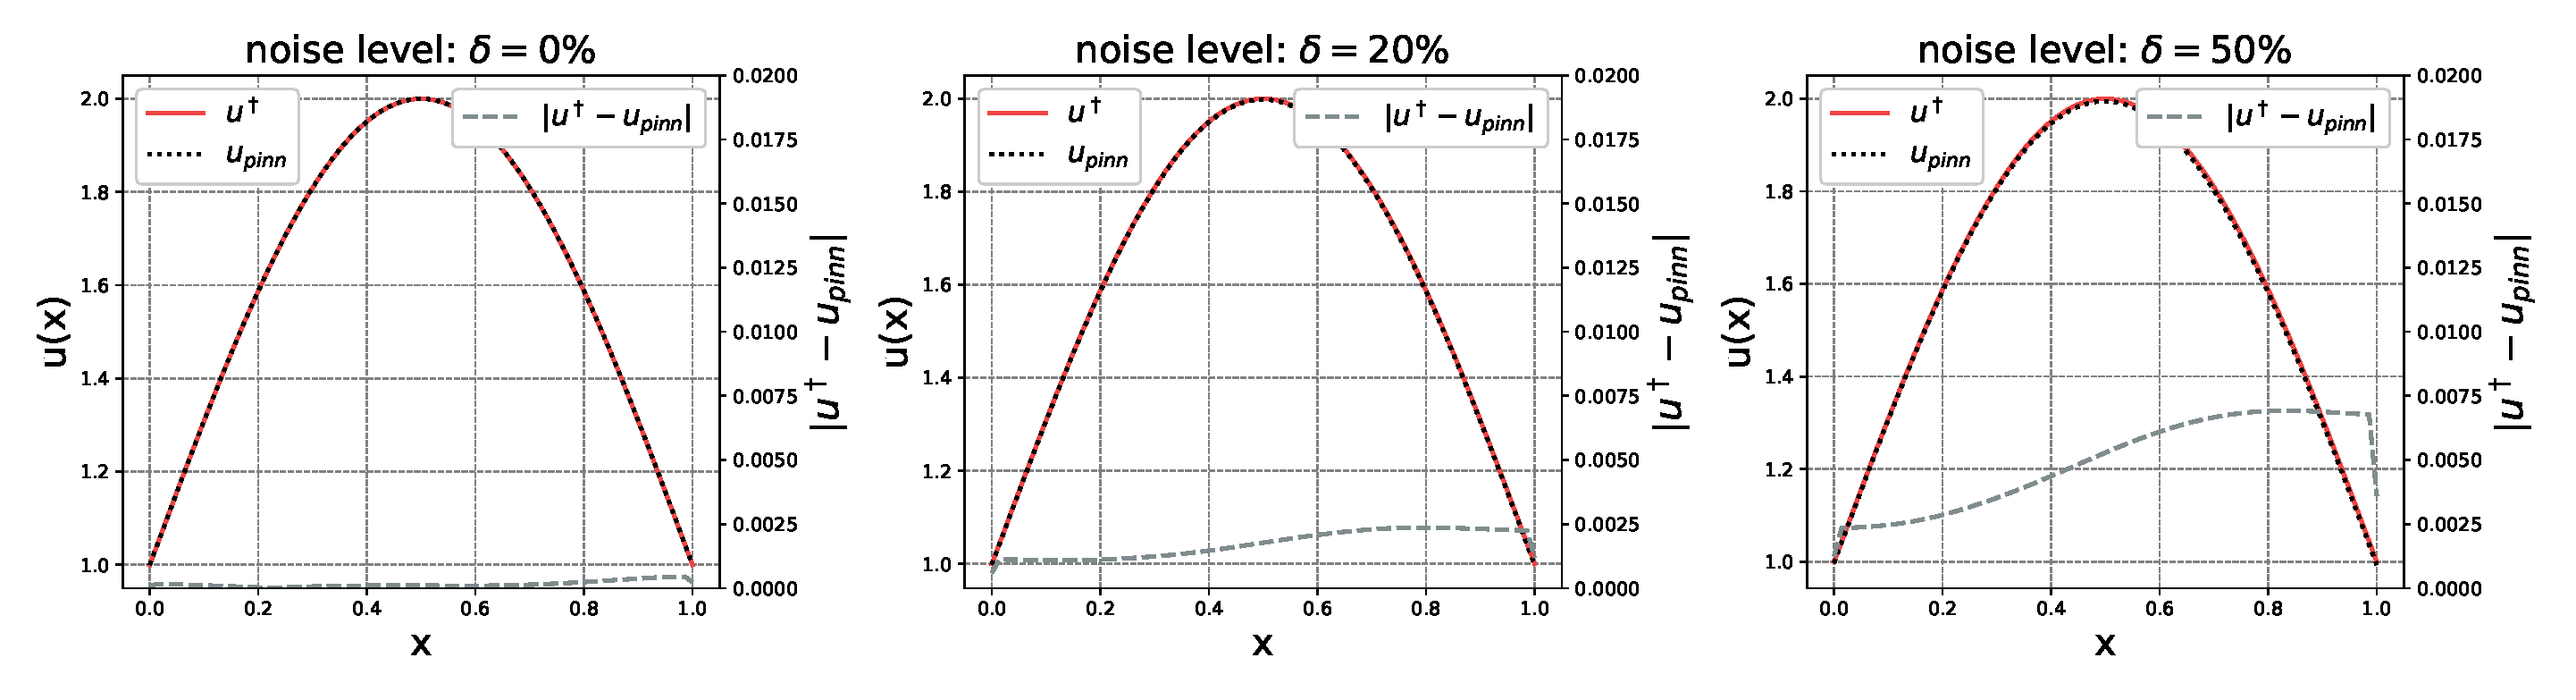
\includegraphics[width=\textwidth]{figures3/ex0_u.eps}
%     \caption{例 \ref{example:1d} 的精确解、Tikhonov-PINN 解和绝对误差。第一行对应源项 $q$，第二行对应解 $u$。从左到右，结果是在不同的噪声水平下获得的。}
%     \label{fig:ex0_q_u}
% \end{figure}

% 在本小节中，我们使用一个一维例子来验证 Tikhonov-PINNs 的收敛率，并研究超参数对重构误差的影响。
% \begin{example}\label{example:1d}
% 令 $\Omega=(0,1)$ 且 $\alpha\equiv 1$，定义精确势函数为 $q^{\dagger}(x)=\exp(x)$，对应的解为 $u^{\dagger}(x) = 1+\sin(\pi x)$。源项 $f$ 和边界条件 $g$ 由模型方程 Eq.\eqref{eq:pde:potential} 确定。
% \end{example}

% $q$ 和 $u$ 的精确解与 Tikhonov-PINNs 解如图 \ref{fig:ex0_q_u} 所示。在本例中，我们设置 $\lambda=10^{-7}$，采样 50,000 个内部点，并将边界点设为 \{0, 1\}。优化使用 Adam 优化器进行，学习率为 $10^{-4}$，迭代次数为 10,000 次。我们采用一个具有 $tanh$ 激活函数且宽度为 64 的两层神经网络来逼近 $q$ 和 $u$，并在架构中每两个相邻隐藏层之间应用残差连接。除非另有说明，本小节中的所有一维算例均使用与本例相同的默认参数设置。

% \subsubsection{收敛率}
% 在定理 \ref{thm:ConvergenceRate} 中，我们建立了 $q$ 和 $u$ 关于噪声水平 $\delta$ 的收敛率。为了验证这一结果，我们计算了不同噪声水平下 $q$ 和 $u$ 的相对误差，结果如图 \ref{fig:ex0:noise} 所示。

% \begin{figure}[htbp]
%     \centering
%     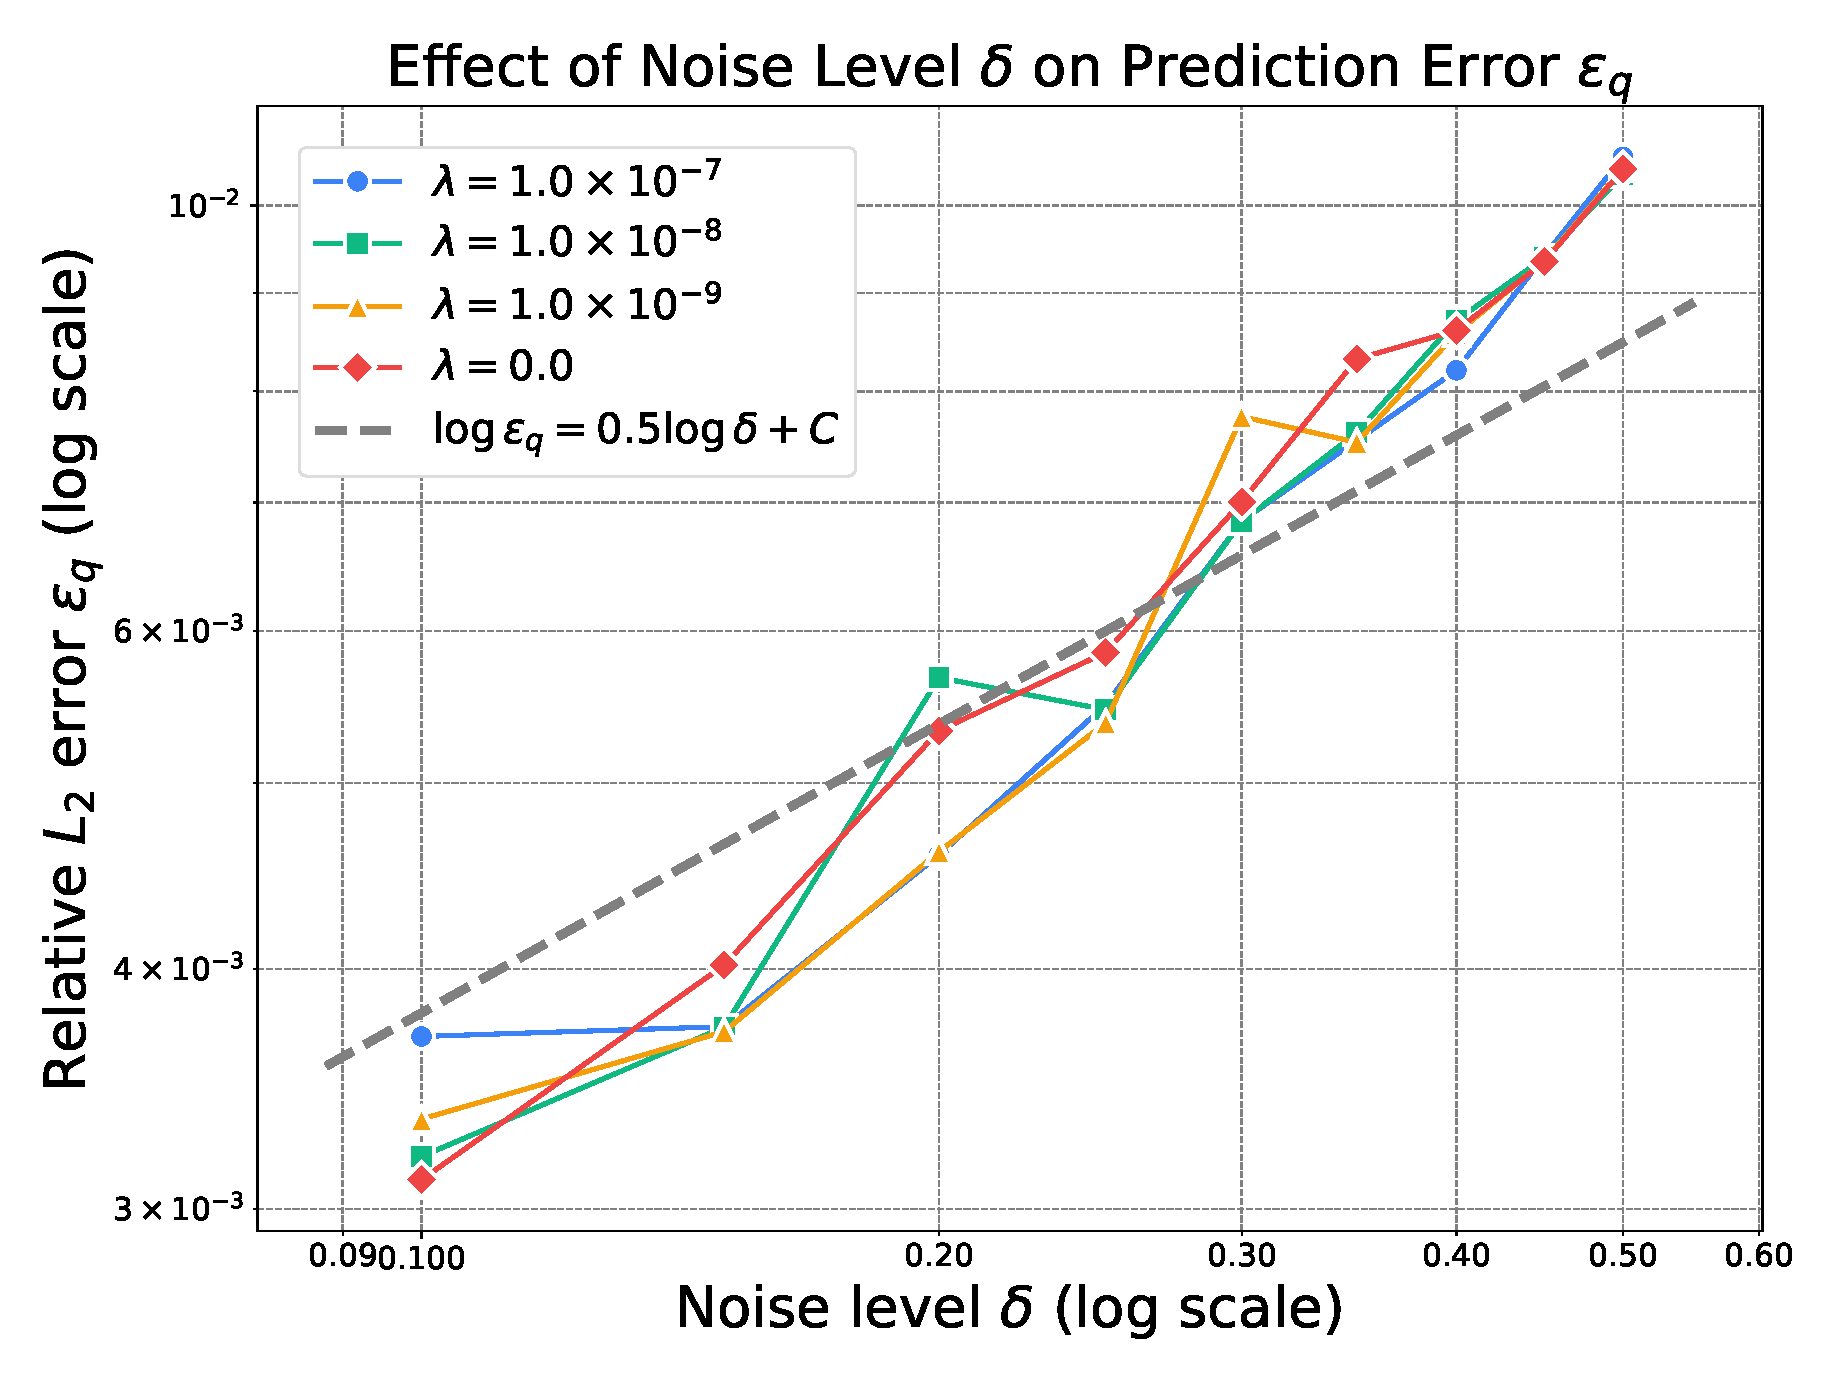
\includegraphics[width=0.49\textwidth]{figures3/ex0_noise_q.eps}
%     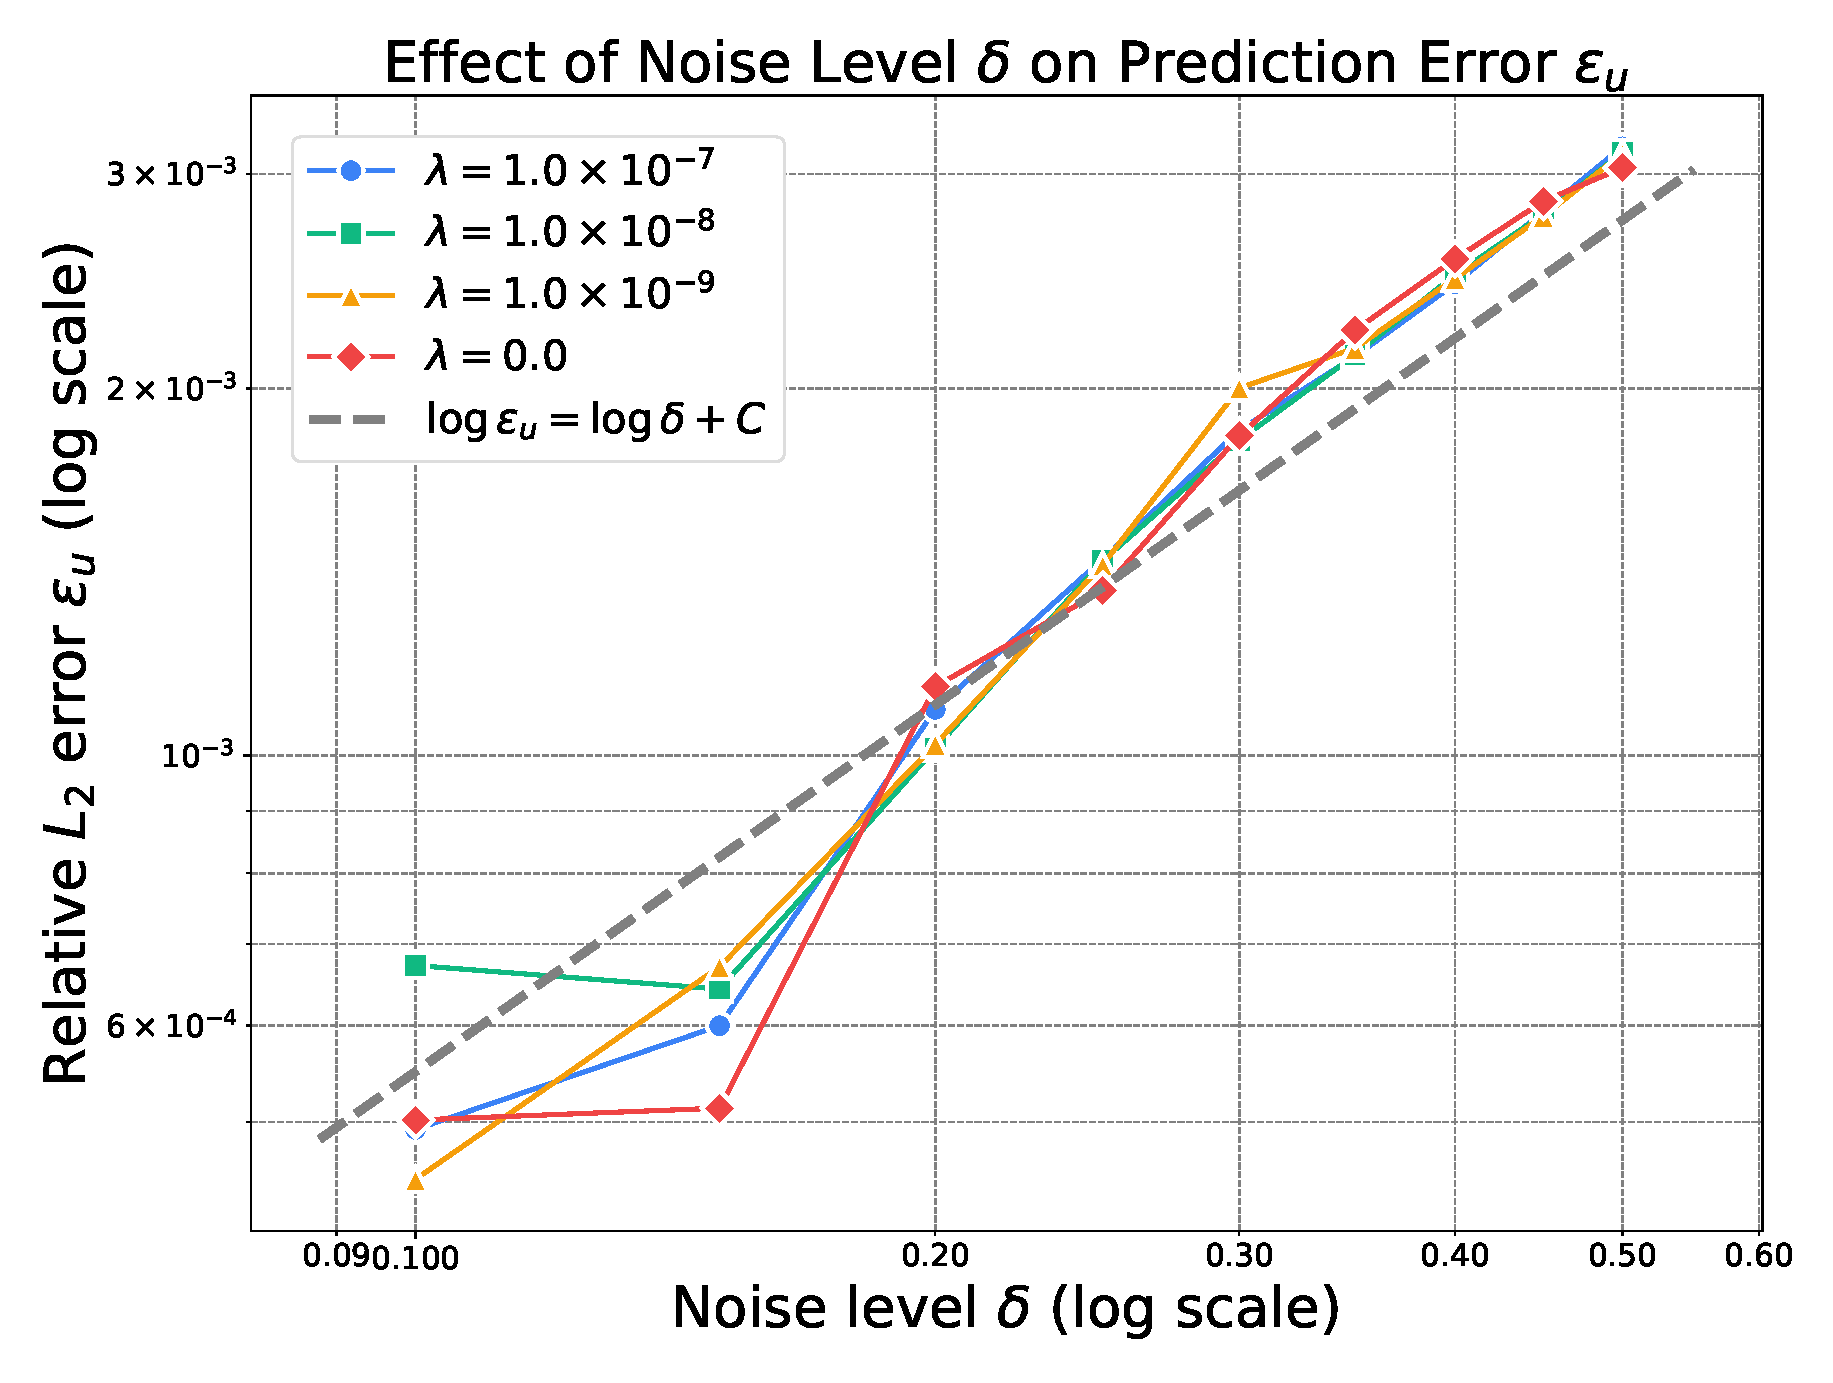
\includegraphics[width=0.49\textwidth]{figures3/ex0_noise_u.eps}
%     \caption{不同正则化参数下噪声水平对解误差的影响。左图显示了 $q$ 的结果，其中 $\lambda=$$10^{-7}$, $10^{-8}$, $10^{-9}$ 和 0 对应的对数回归曲线的斜率分别为 0.708、0.748、0.760 和 0.743，平均斜率为 0.744。右图显示了 $u$ 的结果，其中对应的斜率分别为 1.22、1.08、1.25 和 1.26，平均斜率为 1.21。}
%     \label{fig:ex0:noise}
% \end{figure}

% 由于目标势函数具有正下界，该算例满足 $\beta = 0$ 的正性条件。根据定理~\ref{thm:ConvergenceRate} 和注 \ref{compare_Gar}，$q$ 和 $u$ 的收敛率可以任意接近 $O(\delta^{0.5})$ 和 $O(\delta)$。这一点在图 \ref{fig:ex0:noise} 中得到了检验，其中 $u$ 和 $q$ 的数值收敛率与理论收敛率非常一致。平均而言，在不同的 $\lambda$ 值下，我们观察到 $u$ 的经验收敛率为 $O(\delta^{1.21})$，$q$ 的经验收敛率为 $O(\delta^{0.74})$，这实际上快于理论收敛率，表明我们的理论界可能不是最优的。

% \subsubsection{正则化的影响}
% 在本小节中，我们要研究不同正则化在求解算例 \ref{example:1d} 时的影响。如表 \ref{tab:regularization} 所示，当训练样本量相对较小（表 1 中的第一个子表）时，与 $L^2$ 正则化或原始 PINNs 相比，$H^2$ 正则化显著降低了 $q$ 的相对误差，尤其是当正则化系数 $\lambda$ 相对较大时。第二个子表表明，随着更多训练样本的可用，这种改进变得不那么明显。这是符合预期的，因为适当的正则化和增加数据量都有助于防止过拟合并提高精度。尽管如此，在两种情况下，当 $\lambda$ 选择得当时，$H^2$ 正则化都能产生最小的重构误差。这些结果凸显了 $H^2$ 正则化在求解此类反势问题时的有效性和优越性。

% \begin{table}[hbtp]
% \centering
% \footnotesize
% \caption{算例 \ref{example:1d} 中不同正则化下 $\hat{q}$ 的相对 $L^{2}$ 误差。}
% \begin{tabular}{lrrrrr}
% \hline
% \multirow{2}[0]{*}{$\text{err}(q_{\text{pinn}})$} & \multicolumn{5}{c}{正则化参数 $\lambda$} \\
% \cline{2-6}
% & \multicolumn{1}{l}{$1.0\times 10^{-3}$} & 
% \multicolumn{1}{l}{$1.0\times 10^{-4}$} &
% \multicolumn{1}{l}{$1.0\times 10^{-5}$} &
% \multicolumn{1}{l}{$1.0\times 10^{-6}$} & 
% \multicolumn{1}{l}{$1.0\times 10^{-7}$} \\
%    \hline
% $H^2$ 正则化 & $5.44\times 10^{-2}$ & $\textbf{5.26}\times \textbf{10}^{-2}$ & $8.27\times 10^{-2}$ & $8.99\times 10^{-2}$ & $9.07\times 10^{-2}$ \\
% $L^2$ 正则化 & $9.35\times 10^{-2}$ & $9.11\times 10^{-2}$ & $9.08\times 10^{-2}$ & $9.08\times 10^{-2}$ & $9.08\times 10^{-2}$ \\
% 无正则化 & $9.08\times 10^{-2}$ & $9.08\times 10^{-2}$ & $9.08\times 10^{-2}$ & $9.08\times 10^{-2}$ & $9.08\times 10^{-2}$  \\
% \hline
% &       &       &       &       & \\
% \hline
% \multirow{2}[0]{*}{$\text{err}(q_{\text{pinn}})$} & \multicolumn{5}{c}{正则化参数 $\lambda$} \\
% \cline{2-6}
% & \multicolumn{1}{l}{$1.0\times 10^{-3}$} & 
% \multicolumn{1}{l}{$1.0\times 10^{-4}$} &
% \multicolumn{1}{l}{$1.0\times 10^{-5}$} &
% \multicolumn{1}{l}{$1.0\times 10^{-6}$} & 
% \multicolumn{1}{l}{$1.0\times 10^{-7}$} \\
% \hline
% $H^2$ 正则化 & $8.96\times 10^{-2}$ & $3.14\times 10^{-2}$ & $\textbf{2.94}\times \textbf{10}^{-2}$ & $3.03\times 10^{-2}$ & $3.04\times 10^{-2}$  \\
% $L^2$ 正则化 & $3.80\times 10^{-2}$ & $3.10\times 10^{-2}$ & $3.05\times 10^{-2}$ & $3.04\times 10^{-2}$ & $3.04\times 10^{-2}$ \\
% 无正则化 & $3.04\times 10^{-1}$ & $3.04\times 10^{-2}$ & $3.04\times 10^{-2}$ & $3.04\times 10^{-2}$ & $3.04\times 10^{-2}$ \\
% \hline

% \end{tabular}
% \label{tab:regularization}
% \end{table}

% \subsubsection{其他超参数的影响}

% \begin{figure}[htbp]
%     \centering
%     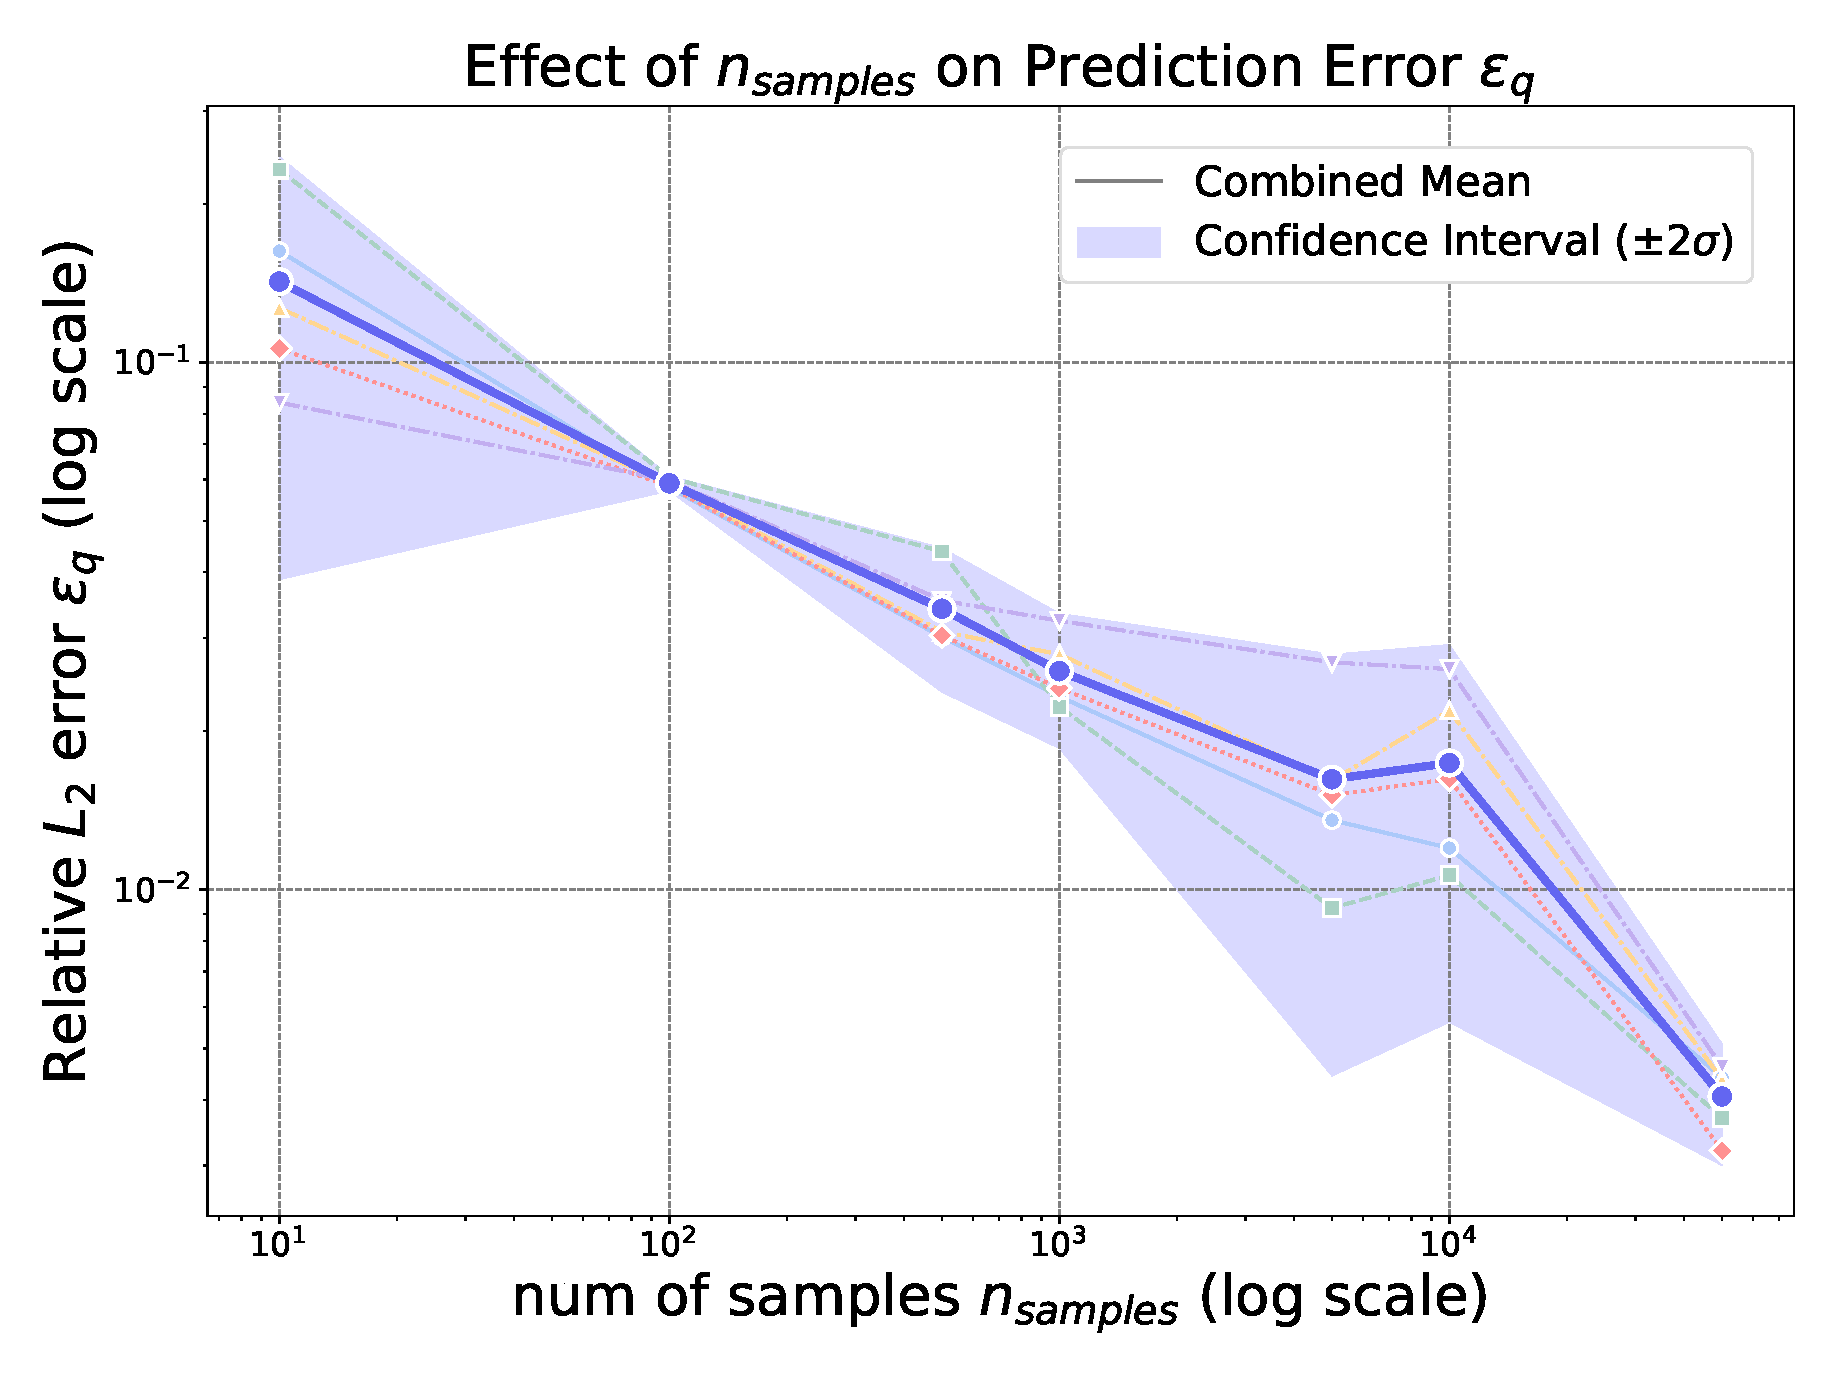
\includegraphics[width=0.48\textwidth]{figures3/ex0_nsample.eps}
%     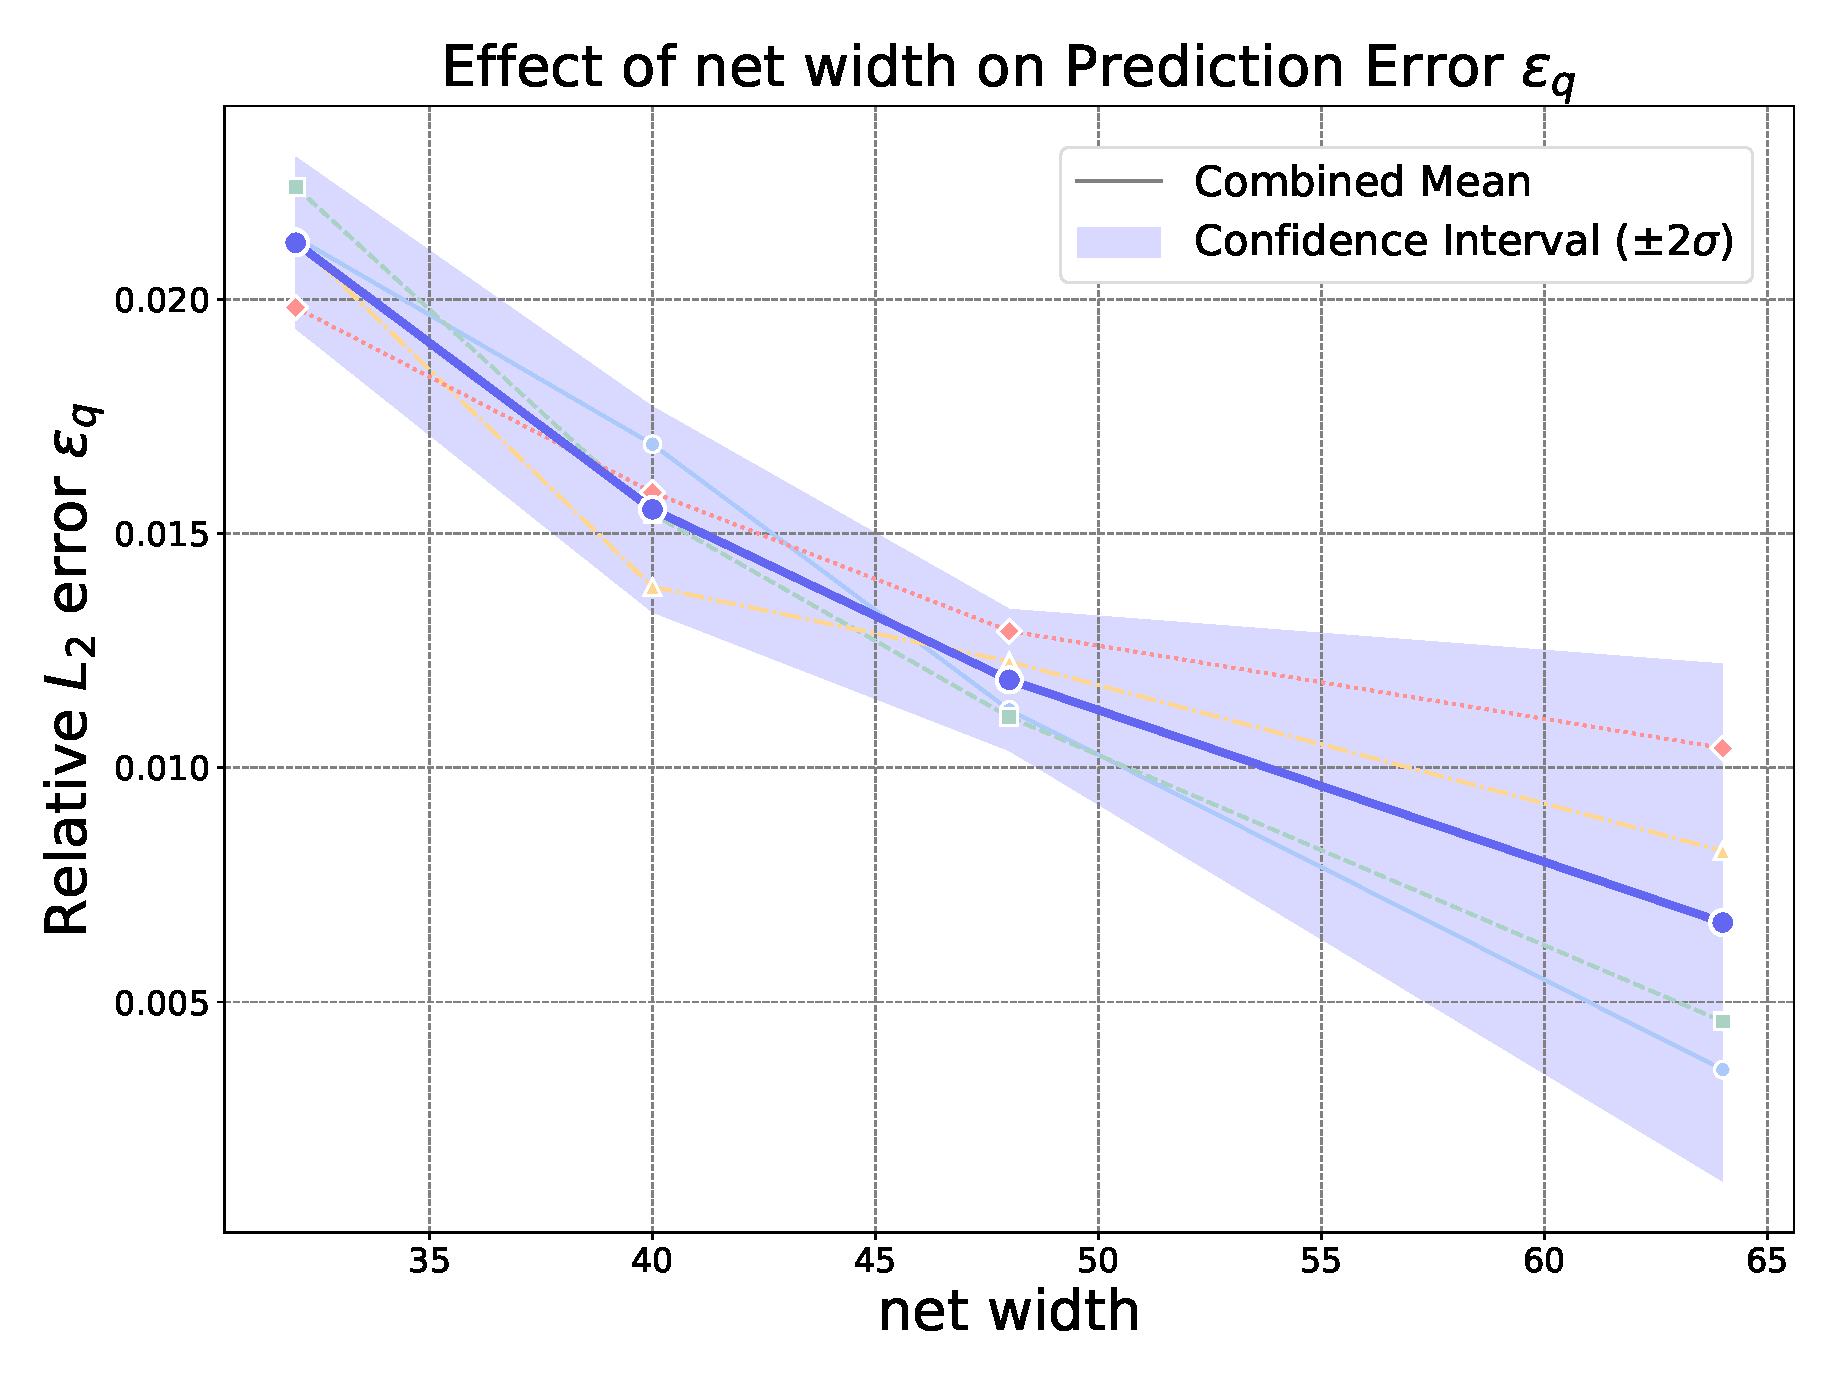
\includegraphics[width=0.48\textwidth]{figures3/ex0_width.eps}
%     \caption{样本大小和网络宽度对算法精度的影响。我们进行了多次运行，并展示了相应的置信区间。特别地，由于网络深度是固定的，非零参数的数量 $R_{\calQ}$ 与网络宽度近似成正比。}
%     \label{fig:ex0:width}
% \end{figure}

% 我们研究了神经网络复杂度和样本复杂度对模型性能的影响。根据定理 \ref{thm:ConvergenceRate} 和假设 \ref{allcondition}，要实现更低的重构误差，需要增加样本大小和网络规模。我们通过以下实验验证了这种单调关系。在图~\ref{fig:ex0:width} 左侧，我们固定网络架构并改变样本大小以考察其影响。在图~\ref{fig:ex0:width} 右侧，我们保持两层的网络深度，同时调整网络宽度，从而按比例缩放神经元总数 $R_\mathbf{\calQ}$。对每个设置都进行了多次运行，图中显示的结果表明，误差随着样本大小和参数数量的增加而减小。

% \subsubsection{二维问题}
% 接下来我们展示一个二维光滑算例，其中待反演的 $q^{\dagger}$ 和 $u^{\dagger}$ 均呈现正弦函数形式。

% \begin{example}\label{example:onemode}
% 令 $\Omega=(0,1)^{2}$ 且 $\alpha\equiv 1$。我们考虑对以下势函数的识别
% \begin{equation*}
% q^{\dagger}(x_{1},x_{2})=1+0.5\times\sin(\pi x_{1})\sin(\pi x_{2}),
% \end{equation*}
% 且精确解 $u^{\dagger}$ 为：
% \[
% u^{\dagger}(x_{1},x_{2})=1+\sin(\pi x_{1})\sin(\pi x_{2}).
% \]
% \end{example}

% 在本实验中，神经网络包含两个宽度为 64 的隐藏层。我们在内部和边界上共采样 100,000 个点，并使用学习率为 $10^{-4}$ 的 Adam 优化器训练模型 50,000 次迭代。

% 我们还使用有限元方法 (FEM) 求解了相同的问题。在 FEM 实现中，采用了一阶拉格朗日单元，并利用 L-BFGS 算法对解进行了 50 次迭代优化。为了确保比较的公平性，区域 $[0,1]^2$ 被离散化为 $320\times 320=102,400$ 个网格点，这与 Tikhonov-PINNs 中使用的总样本数（$100,000$ 个样本）相当。

% \begin{figure}[htbp]
%     \centering
%     % 第一个子图：Tikhonov-PINNs 方法（假设文件名暗示这是神经网络方法）
%     \begin{subfigure}[b]{\textwidth}
%         \centering
%         % 插入图片
%         \includegraphics[width=\textwidth]{figures3/one_peak_nn.eps}
%         % 简短的子标题
%         \caption{Tikhonov-PINNs 方法结果}
%         \label{fig:one_peak_nn}
%     \end{subfigure}
%     \hfill % 填充中间空白，让图片分别对齐左右
%     % 第二个子图：有限元方法 (FEM)
%     \begin{subfigure}[b]{\textwidth}
%         \centering
%         % 插入图片
%         \includegraphics[width=\textwidth]{figures3/one_peak_fem.eps}
%         % 简短的子标题
%         \caption{有限元方法 (FEM) 结果}
%         \label{fig:one_peak_fem}
%     \end{subfigure}
    
%     % 总标题：包含详细描述
%     \caption{两种方法重构结果的比较：(a) Tikhonov-PINNs 和 (b) 有限元方法 (FEM)。
%     左侧小图展示了例 \ref{example:onemode} 中势函数 $q^{\dagger}$（上）和解 $u^{\dagger}$（下）的真值；
%     右侧小图展示了在不同噪声水平 $\delta$ 下，使用最优正则化参数 $\lambda$ 重构的势 $\hat{q}$ 和解 $\hat{u}$。}
%     \label{fig:example:one_peak}
% \end{figure}


% 数值结果如图~\ref{fig:example:one_peak} 所示。这里，基于各种实验，$\lambda$ 被选为最优正则化参数。为了进一步阐明噪声 $\delta$ 的影响，我们在表~\ref{tab:onemode} 中提供了不同正则化参数 $\lambda$ 下相对误差的详细比较。显然，在低噪声水平下，FEM 和 Tikhonov-PINNs 方法均能有效地重构 $q$ 和 $u$。此外，随着噪声水平的增加，$q$ 的误差逐渐增大，这与我们的理论发现相符。在大多数情况下，FEM 优于 Tikhonov-PINNs 方法，当 $\lambda$ 选择得当时，产生的相对 $L^2$ 误差更低。这突显了 FEM 在处理此类光滑问题时的优越性，特别是在低维情况下。然而，正如第~\ref{sec:semi_converge} 节所讨论的，FEM 中的半收敛现象需要仔细的早停策略。此外，对于非光滑和高维问题，Tikhonov-PINNs 表现出优于标准 FEM 的性能。我们将在后续章节中对此进行讨论。

% 聚焦于 Tikhonov-PINNs 的结果，很明显，较高的噪声水平需要较大的正则化参数 $\lambda$，以在重构解中获得最佳的误差控制。噪声强度与正则化参数之间的这种单调关系与定理~\ref{thm:ConvergenceRate} 中的分析一致。

% \begin{table}[htbp]
%    \centering
%    \footnotesize
%    \caption{例 \ref{example:onemode} 中重构势 $\hat{q}$ 和解 $\hat{u}$ 的相对 $L^{2}$ 误差。}
%    \begin{tabular}{lllllll}
%    \hline
%    \multirow{2}[0]{*}{$\delta  = 1\%$} & \multicolumn{6}{c}{正则化参数 $\lambda$} \\
%    \cline{2-7}
%    & $1.0\times 10^{-5}$ & $1.0\times 10^{-6}$ & $1.0\times 10^{-7}$ & $1.0\times 10^{-8}$ & $1.0\times 10^{-9}$ & \multicolumn{1}{r}{0} \\
%    \hline
%    $\text{err}(u_{\text{pinn}})$ & $3.14\times 10^{-3}$ & $1.49\times 10^{-3}$ & $7.67\times 10^{-4}$ & $5.99\times 10^{-4}$ & $5.81\times 10^{-4}$ & $5.72\times 10^{-4}$ \\
%    $\text{err}(u_{\text{fem}})$ & $1.93\times 10^{-4}$ & $1.84\times 10^{-4}$ & $1.19\times 10^{-4}$ & $1.44\times 10^{-4}$ & $1.68\times 10^{-4}$ & $1.03\times 10^{-4}$ \\
%    $\text{err}(q_{\text{pinn}})$ & $1.46\times 10^{-1}$ & $5.39\times 10^{-2}$ & $3.39\times 10^{-2}$ & $3.27\times 10^{-2}$ & $3.27\times 10^{-2}$ & $3.27\times 10^{-2}$ \\
%    $\text{err}(q_{\text{fem}})$ & $1.44\times 10^{-2}$ & \textbf{1.23$\times $10$^{-2}$} & $6.26\times 10^{-3}$ & $1.27\times 10^{-2}$ & $1.68\times 10^{-2}$ & $1.95\times 10^{-2}$ \\
%    \hline
%    &       &       &       &       &       &  \\
%    \hline
%    \multirow{2}[0]{*}{$\delta = 10\%$} & \multicolumn{6}{c}{正则化参数 $\lambda$} \\
%    \cline{2-7}
%    & $1.0\times 10^{-5}$ & $1.0\times 10^{-6}$ & $1.0\times 10^{-7}$ & $1.0\times 10^{-8}$ & $1.0\times 10^{-9}$ & \multicolumn{1}{r}{0} \\
%    \hline
%    $\text{err}(u_{\text{pinn}})$ & $3.08\times 10^{-3}$ & $1.97\times 10^{-3}$ & $1.48\times 10^{-3}$ & $1.41\times 10^{-3}$ & $1.40\times 10^{-3}$ & $1.40\times 10^{-3}$ \\
%    $\text{err}(u_{\text{fem}})$ & $1.09\times 10^{-3}$ & $6.30\times 10^{-4}$ & $1.71\times 10^{-3}$ & $2.51\times 10^{-3}$ & $2.71\times 10^{-3}$ & $3.43\times 10^{-3}$\\
%    $\text{err}(q_{\text{pinn}})$ & $1.50\times 10^{-1}$ & $6.18\times 10^{-2}$ & $4.33\times 10^{-2}$ & $4.13\times 10^{-2}$ & $4.11\times 10^{-2}$ & $4.11\times 10^{-2}$ \\
%    $\text{err}(q_{\text{fem}})$ & \textbf{1.72$\times $10$^{-2}$} & $2.84\times 10^{-2}$ & $8.56\times 10^{-2}$ & $3.23\times 10^{-1}$ & $3.80\times 10^{-1}$ & $5.40\times 10^{-1}$\\
%    \hline
%    &       &       &       &       &       &  \\
%    \hline
%    \multirow{2}[0]{*}{$\delta = 20\%$} & \multicolumn{6}{c}{正则化参数 $\lambda$} \\
%    \cline{2-7}
%    & $1.0\times 10^{-5}$ & $1.0\times 10^{-6}$ & $1.0\times 10^{-7}$ & $1.0\times 10^{-8}$ & $1.0\times 10^{-9}$ & \multicolumn{1}{r}{0} \\
%    \hline
%    $\text{err}(u_{\text{pinn}})$ & $3.38\times 10^{-3}$ & $2.47\times 10^{-3}$ & $2.19\times 10^{-3}$ & $2.17\times 10^{-3}$ & $2.17\times 10^{-3}$ & $2.17\times 10^{-3}$ \\
%    $\text{err}(u_{\text{fem}})$ & $8.88\times 10^{-4}$ & $2.16\times 10^{-3}$ & $4.76\times 10^{-3}$ & $4.30\times 10^{-3}$ & $3.44\times 10^{-3}$ & $4.98\times 10^{-3}$ \\
%    $\text{err}(q_{\text{pinn}})$ & $1.54\times 10^{-1}$ & $7.29\times 10^{-2}$ & $6.34\times 10^{-2}$ & $6.44\times 10^{-2}$ & $6.46\times 10^{-2}$ & $6.46\times 10^{-2}$ \\
%    $\text{err}(q_{\text{fem}})$ & \textbf{1.89$\times $10$^{-2}$} & $8.56\times 10^{-2}$ & $2.64\times 10^{-1}$ & $3.85\times 10^{-1}$ & $4.35\times 10^{-1}$ & $4.98\times 10^{-1}$\\
%    \hline
%    &       &       &       &       &       &  \\
%    \hline
%    \multirow{2}[0]{*}{$\delta = 50\%$} & \multicolumn{6}{c}{正则化参数 $\lambda$} \\
%    \cline{2-7}
%    & $1.0\times 10^{-5}$ & $1.0\times 10^{-6}$ & $1.0\times 10^{-7}$ & $1.0\times 10^{-8}$ & $1.0\times 10^{-9}$ & \multicolumn{1}{r}{0} \\
%    \hline
%    $\text{err}(u_{\text{pinn}})$ & $4.14\times 10^{-3}$ & $5.22\times 10^{-3}$ & $5.20\times 10^{-3}$ & $5.22\times 10^{-3}$ & $5.22\times 10^{-3}$ & $5.22\times 10^{-3}$ \\
%    $\text{err}(u_{\text{fem}})$ & $4.90\times 10^{-3}$ & $7.22\times 10^{-3}$ & $8.26\times 10^{-3}$ & $1.01\times 10^{-2}$ & $1.40\times 10^{-2}$ & $9.21\times 10^{-3}$ \\
%    $\text{err}(q_{\text{pinn}})$ & $1.65\times 10^{-1}$ & $1.03\times 10^{-1}$ & $1.05\times 10^{-1}$ & $1.06\times 10^{-1}$ & $1.06\times 10^{-1}$ & $1.06\times 10^{-1}$ \\
%    $\text{err}(q_{\text{fem}})$ & \textbf{5.64$\times $10$^{-2}$} & $2.32\times 10^{-1}$ & $5.85\times 10^{-1}$ & $0.85\times 10^{-1}$ & $1.10$ & $0.81\times 10^{-1}$\\
%    \hline
%    \end{tabular}
%    \label{tab:onemode}%
% \end{table}%

% \subsection{非光滑势问题}
% 为了进一步探索我们算法的局限性并评估神经网络对非光滑势的逼近能力，我们将我们的方法应用于几个非光滑算例，在这些算例中，诸如标准有限元方法 (FEM) 等传统方法的效果可能较差。参数设置保持与算例~\ref{example:onemode} 中相同。此外，我们将 Tikhonov-PINNs 方法的性能与经典有限元方法进行了比较。本节的 FEM 设置与算例 5.2 中的设置相同。

% \subsubsection{连续问题}
% 接下来，我们考虑如下定义的非光滑势函数的识别问题。

% \begin{example}\label{example:nonsmooth}
% % Table generated by Excel2LaTeX from sheet '5'
% 令 $\Omega=(0,1)^{2}$ 且 $\alpha\equiv 1$。定义精确势函数 $q^{\dagger}$ 为：
% \begin{align*}
% \zeta(x_{1},x_{2})&=\exp\{-25\times(x_{1}-0.6)^{2}-25\times(x_{2}-0.4)^{2}\}, \\
% q^{\dagger}(x_{1},x_{2})&=0.75+\min\{0.75,\max\{0.25,2\zeta(x_{1},x_{2})\}\},
% \end{align*}
% 精确解 $u^{\dagger}$ 为 $u^{\dagger}(x_{1},x_{2})=1+\sin(\pi x_{1})\sin(\pi x_{2})$。
% \end{example}
% 表 \ref{tab:nonsmooth} 展示了在不同 $\lambda$ 和 $\delta$ 下 $u$ 和 $q$ 的相对误差，并用粗体高亮了每种噪声水平下的最佳结果。正如我们所见，Tikhonov-PINNs 在所有配置下始终实现了约为 $\calO(10^{-2})$ 的 $q$ 相对误差，比有限元方法高出一个数量级。


% \begin{table}[htbp]
%    \centering
%    \footnotesize
%    \caption{Example \ref{example:nonsmooth} 中恢复的势 $\hat{q}$ 和解 $\hat{u}$ 的相对 $L^{2}$ 误差。}
%    \begin{tabular}{lllllll}
%    \hline
%    \multirow{2}[0]{*}{$\delta  = 1\%$} & \multicolumn{6}{c}{正则化参数 $\lambda$} \\
%    \cline{2-7}
%    & $1.0\times 10^{-5}$ & $1.0\times 10^{-6}$ & $1.0\times 10^{-7}$ & $1.0\times 10^{-8}$ & $1.0\times 10^{-9}$ & \multicolumn{1}{r}{0} \\
%    \hline
%    $\text{err}(u_{\text{pinn}})$ & $3.14\times 10^{-3}$ & $2.01\times 10^{-3}$ & $6.03\times 10^{-4}$ & $5.71\times 10^{-4}$ & $4.94\times 10^{-4}$ & $4.03\times 10^{-4}$ \\
%    $\text{err}(u_{\text{fem}})$& $2.60\times 10^{-3}$& $1.14\times 10^{-3}$& $7.09\times 10^{-4}$& $6.96\times 10^{-4}$ & $5.33\times 10^{-4}$ &$6.41\times 10^{-4}$\\
%    $\text{err}(q_{\text{pinn}})$ & $1.46\times 10^{-1}$& $9.63\times 10^{-2}$ & $1.82\times 10^{-2}$ & $1.60\times 10^{-2}$ & \textbf{1.57$\times$ 10$^{-2}$} & \textbf{1.57$\times$ 10$^{-2}$}   \\
%    $\text{err}(q_{\text{fem}})$& $1.28\times 10^{-1}$& $8.77\times 10^{-2}$& $7.39\times 10^{-2}$& $7.36\times 10^{-2}$ & $6.43\times 10^{-2}$ &$6.97\times 10^{-2}$\\
%    \hline
%    &       &       &       &       &       &  \\
%    \hline
%    \multirow{2}[0]{*}{$\delta = 10\%$} & \multicolumn{6}{c}{正则化参数 $\lambda$} \\
%    \cline{2-7}
%    & $1.0\times 10^{-5}$ & $1.0\times 10^{-6}$ & $1.0\times 10^{-7}$ & $1.0\times 10^{-8}$ & $1.0\times 10^{-9}$ & \multicolumn{1}{r}{0} \\
%    \hline
%    $\text{err}(u_{\text{pinn}})$ & $3.08\times 10^{-3}$ & $2.22\times 10^{-3}$ & $1.36\times 10^{-3}$ & $1.30\times 10^{-3}$ & $1.30\times 10^{-3}$ & $1.30\times 10^{-3}$ \\
%    $\text{err}(u_{\text{fem}})$& $2.82\times 10^{-3}$& $1.30\times 10^{-3}$& $1.44\times 10^{-3}$& $1.18\times 10^{-3}$ & $1.30\times 10^{-3}$&$2.36\times 10^{-3}$\\
%    $\text{err}(q_{\text{pinn}})$ & $1.50\times 10^{-1}$ & $1.03\times 10^{-1}$ & $1.78\times 10^{-2}$ & $1.60\times 10^{-2}$ & $1.71\times 10^{-2}$ & \textbf{1.58$\times$ 10$^{-2}$ }\\
%    $\text{err}(q_{\text{fem}})$& $1.29\times 10^{-1}$& $8.77\times 10^{-2}$& $7.95\times 10^{-2}$& $9.02\times 10^{-2}$ & $1.16\times 10^{-1}$&$1.90\times 10^{-1}$\\
%    \hline
%    &       &       &       &       &       &  \\
%    \hline
%    \multirow{2}[0]{*}{$\delta = 20\%$} & \multicolumn{6}{c}{正则化参数 $\lambda$} \\
%    \cline{2-7}
%    & $1.0\times 10^{-5}$ & $1.0\times 10^{-6}$ & $1.0\times 10^{-7}$ & $1.0\times 10^{-8}$ & $1.0\times 10^{-9}$ & \multicolumn{1}{r}{0} \\
%    \hline
%    $\text{err}(u_{\text{pinn}})$ & $3.38\times 10^{-3}$ & $2.30\times 10^{-3}$ & $1.44\times 10^{-3}$ & $1.35\times 10^{-3}$ & $1.36\times 10^{-3}$ & $1.36\times 10^{-3}$ \\
%    $\text{err}(u_{\text{fem}})$& $2.67\times 10^{-3}$& $2.17\times 10^{-3}$& $4.23\times 10^{-3}$&$ 3.75\times 10^{-3}$ & $2.50\times 10^{-3}$&$4.15\times 10^{-3}$\\
%    $\text{err}(q_{\text{pinn}})$ & $1.54\times 10^{-1}$ & $9.09\times 10^{-2}$ & $1.71\times 10^{-2}$ & $1.60\times 10^{-2}$ & \textbf{1.59$\times$ 10$^{-2}$} & \textbf{1.59$\times$ 10$^{-2}$} \\
%    $\text{err}(q_{\text{fem}})$& $1.27\times 10^{-1}$& $9.77\times 10^{-2}$& $2.21\times 10^{-1}$& $2.13\times 10^{-1}$ & $1.51\times 10^{-1}$&$3.79\times 10^{-1}$\\
%    \hline
%    &       &       &       &       &       &  \\
%    \hline
%    \multirow{2}[0]{*}{$\delta = 50\%$} & \multicolumn{6}{c}{正则化参数 $\lambda$} \\
%    \cline{2-7}
%    & $1.0\times 10^{-5}$ & $1.0\times 10^{-6}$ & $1.0\times 10^{-7}$ & $1.0\times 10^{-8}$ & $1.0\times 10^{-9}$ & \multicolumn{1}{r}{0} \\
%    \hline
%    $\text{err}(u_{\text{pinn}})$ & $4.14\times 10^{-3}$ & $4.43\times 10^{-3}$ & $4.07\times 10^{-3}$ & $3.43\times 10^{-3}$ & $4.01\times 10^{-3}$ & $4.04\times 10^{-3}$ \\
%    $\text{err}(u_{\text{fem}})$& $4.41\times 10^{-3}$& $7.14\times 10^{-3}$& $7.90\times 10^{-3}$& $7.64\times 10^{-3}$& $1.26\times 10^{-2}$&$8.40\times 10^{-3}$\\
%    $\text{err}(q_{\text{pinn}})$ & $1.65\times 10^{-1}$ & $1.22\times 10^{-1}$ & $6.30\times 10^{-2}$ & \textbf{3.16}$\times$ \textbf{10}$^{-2}$ & $4.99\times 10^{-2}$ & $5.14\times 10^{-1}$ \\
%    $\text{err}(q_{\text{fem}})$& $1.45\times 10^{-1}$& $2.14\times 10^{-1}$& $4.64\times 10^{-1}$& $4.09\times 10^{-1}$& $9.07\times 10^{-1}$&$5.90\times 10^{-1}$\\
%    \hline
%    \end{tabular}%
%    \label{tab:nonsmooth}%
% \end{table}%

% \begin{figure}[htbp]
% \centering
% \setlength{\abovecaptionskip}{10pt}
% 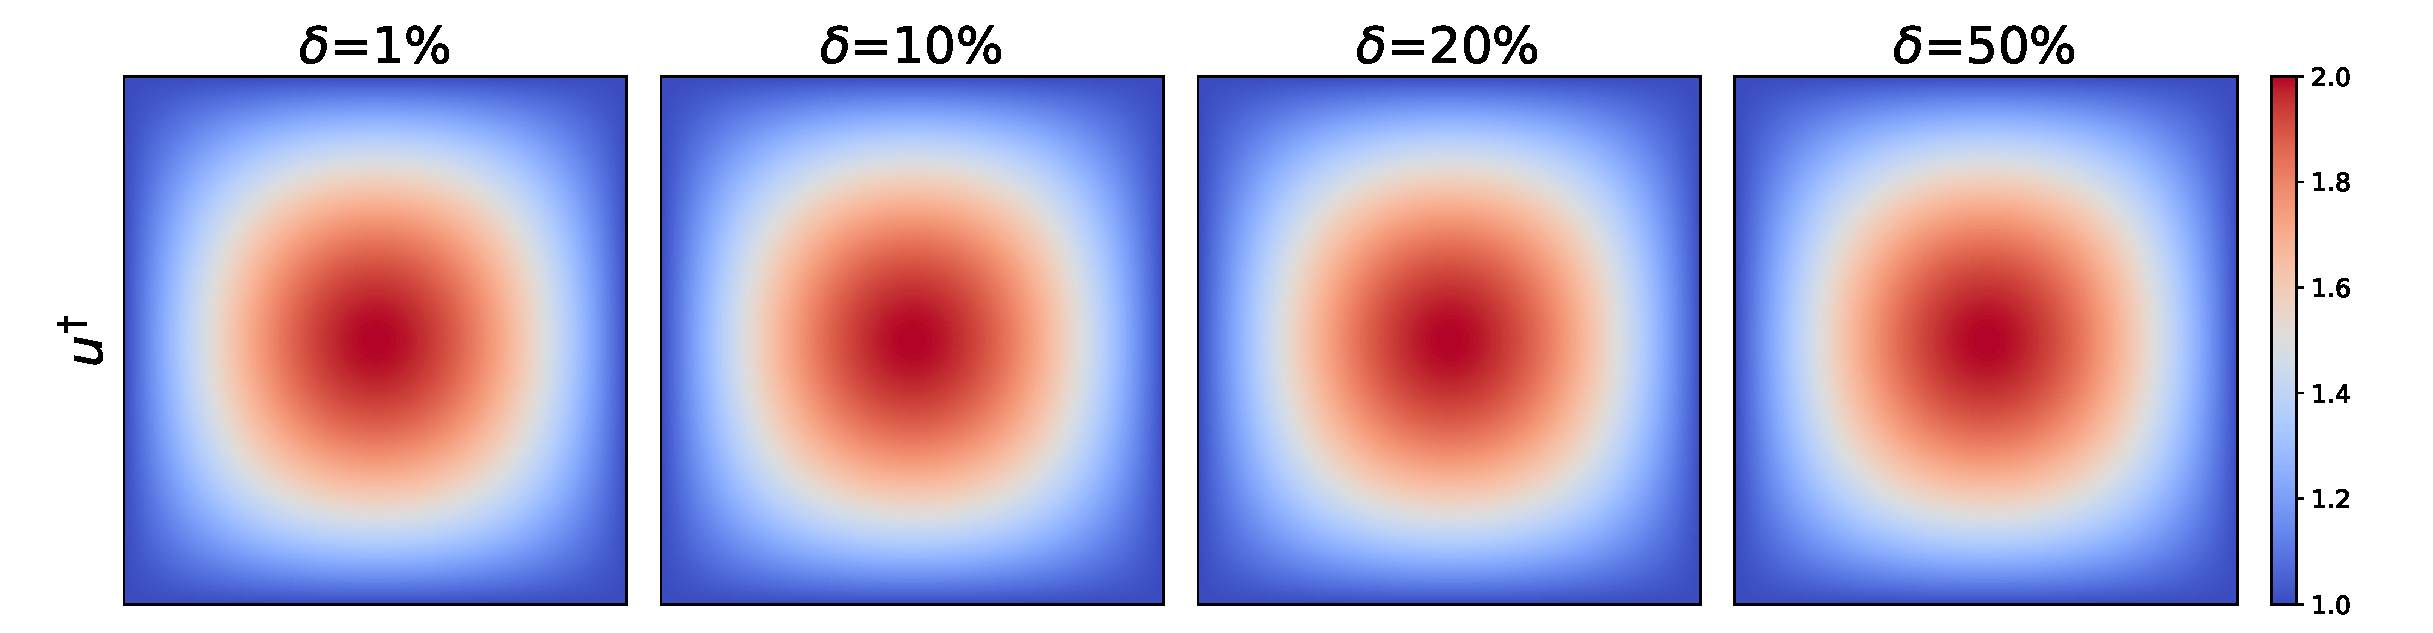
\includegraphics[width=\textwidth]{figures3/non_smooth_udag.eps}\par
% 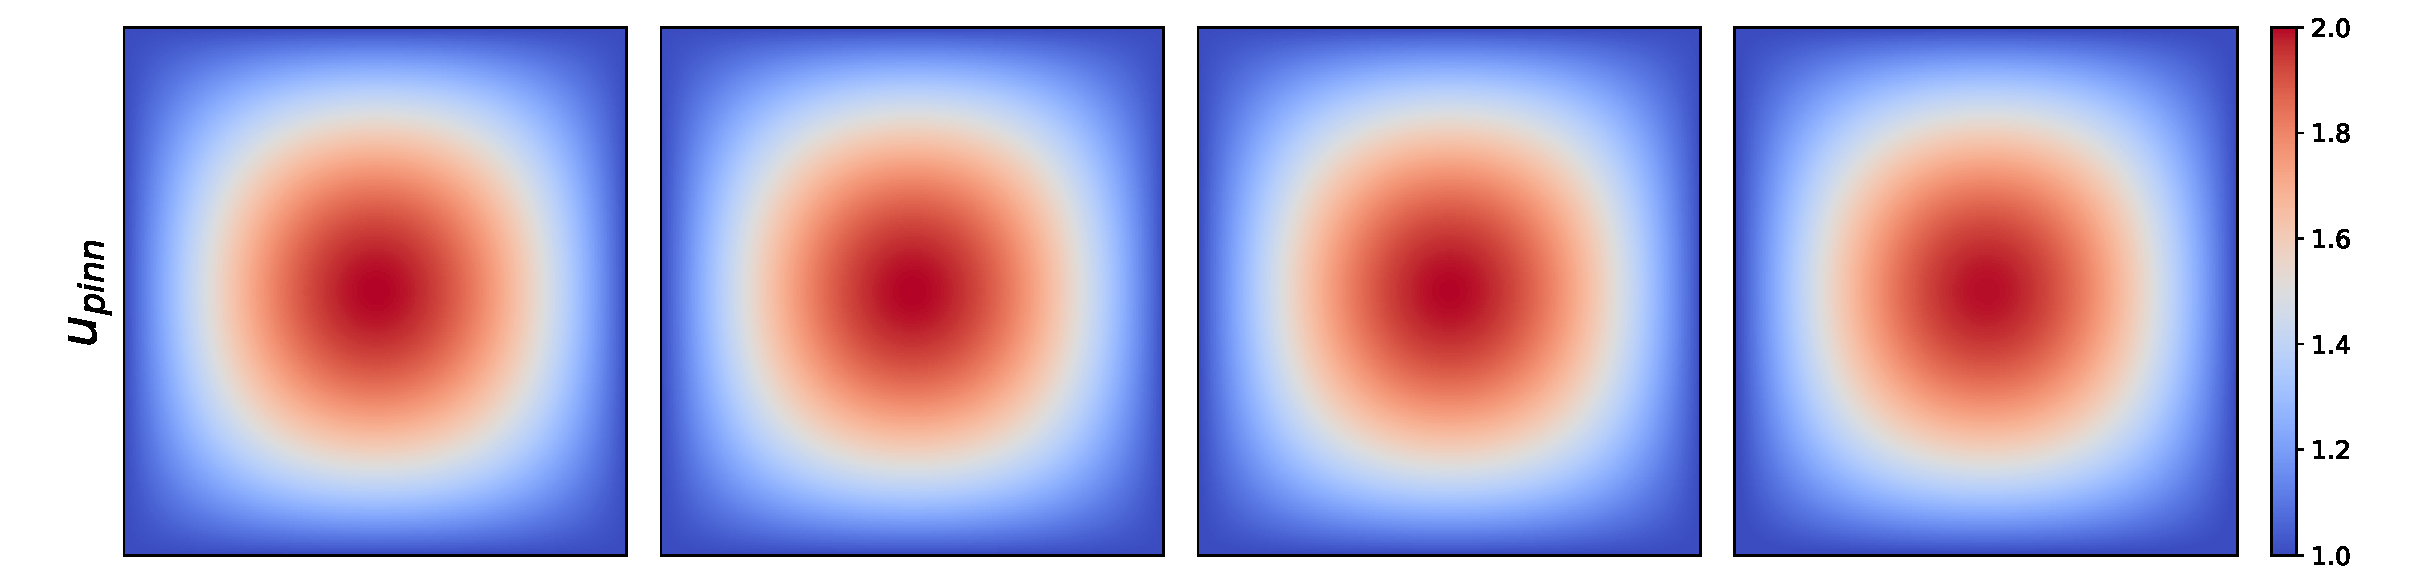
\includegraphics[width=\textwidth]{figures3/non_smooth_unn.eps}\par
% 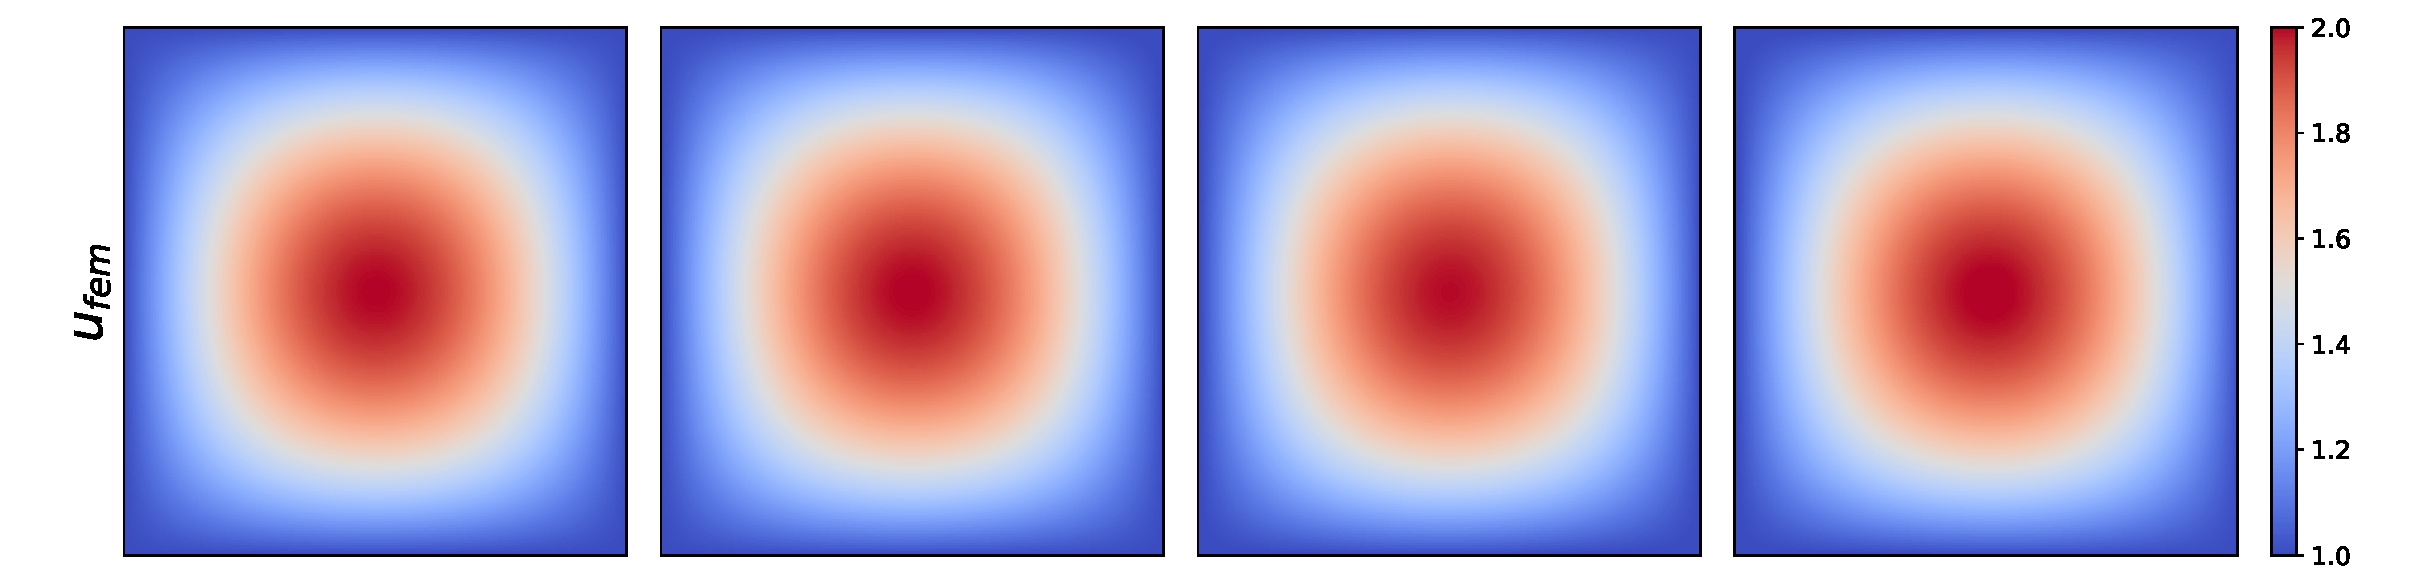
\includegraphics[width=\textwidth]{figures3/non_smooth_ufem.eps}\par
% 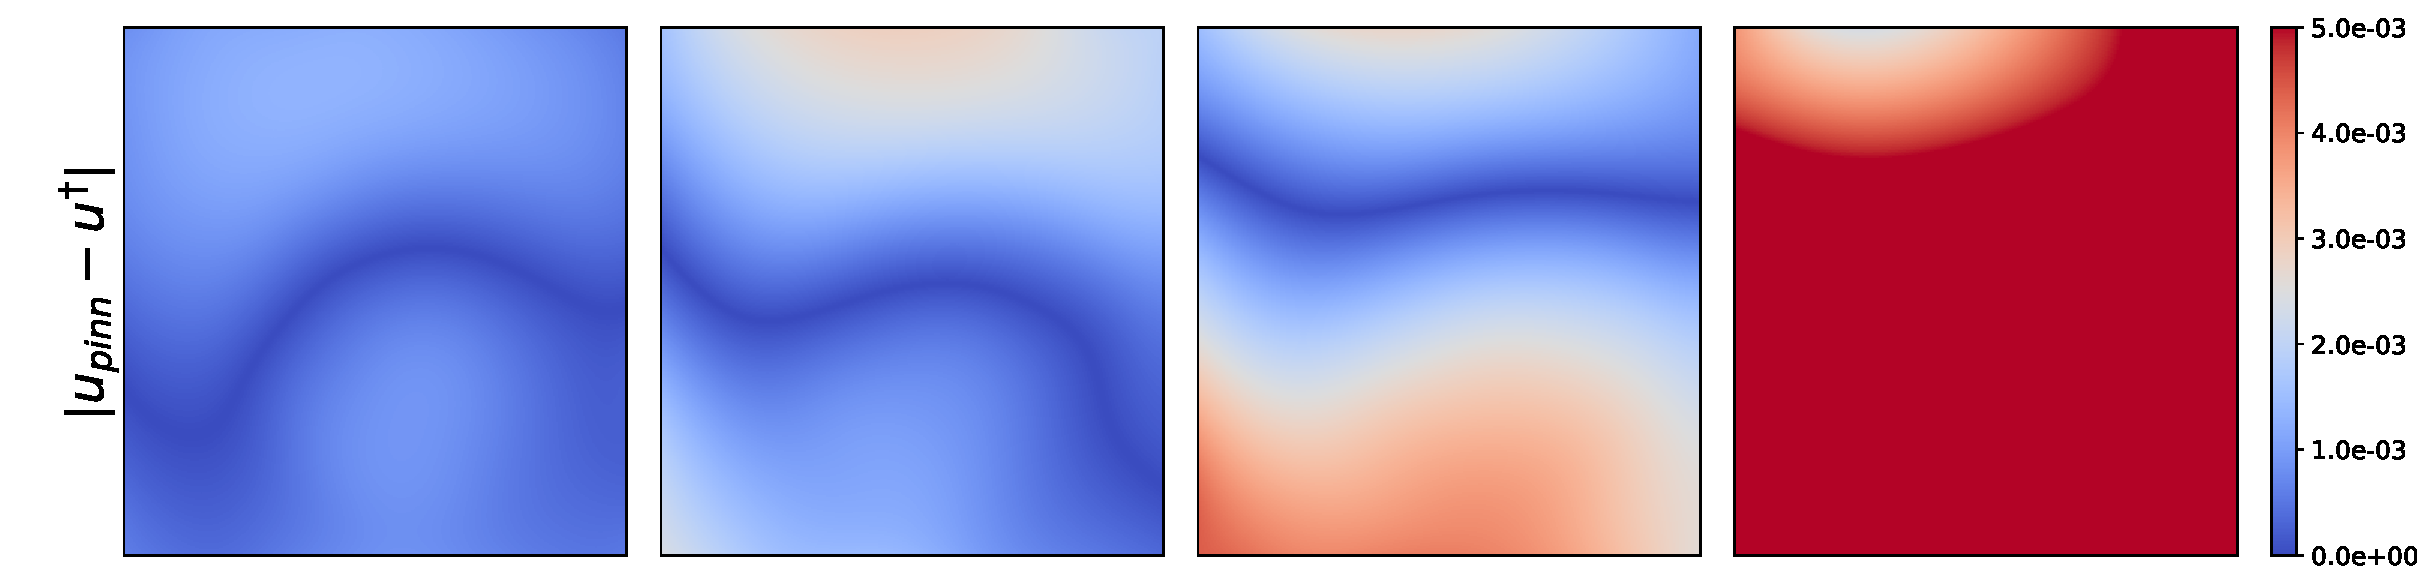
\includegraphics[width=\textwidth]{figures3/non_smooth_unn_err.eps}\par
% 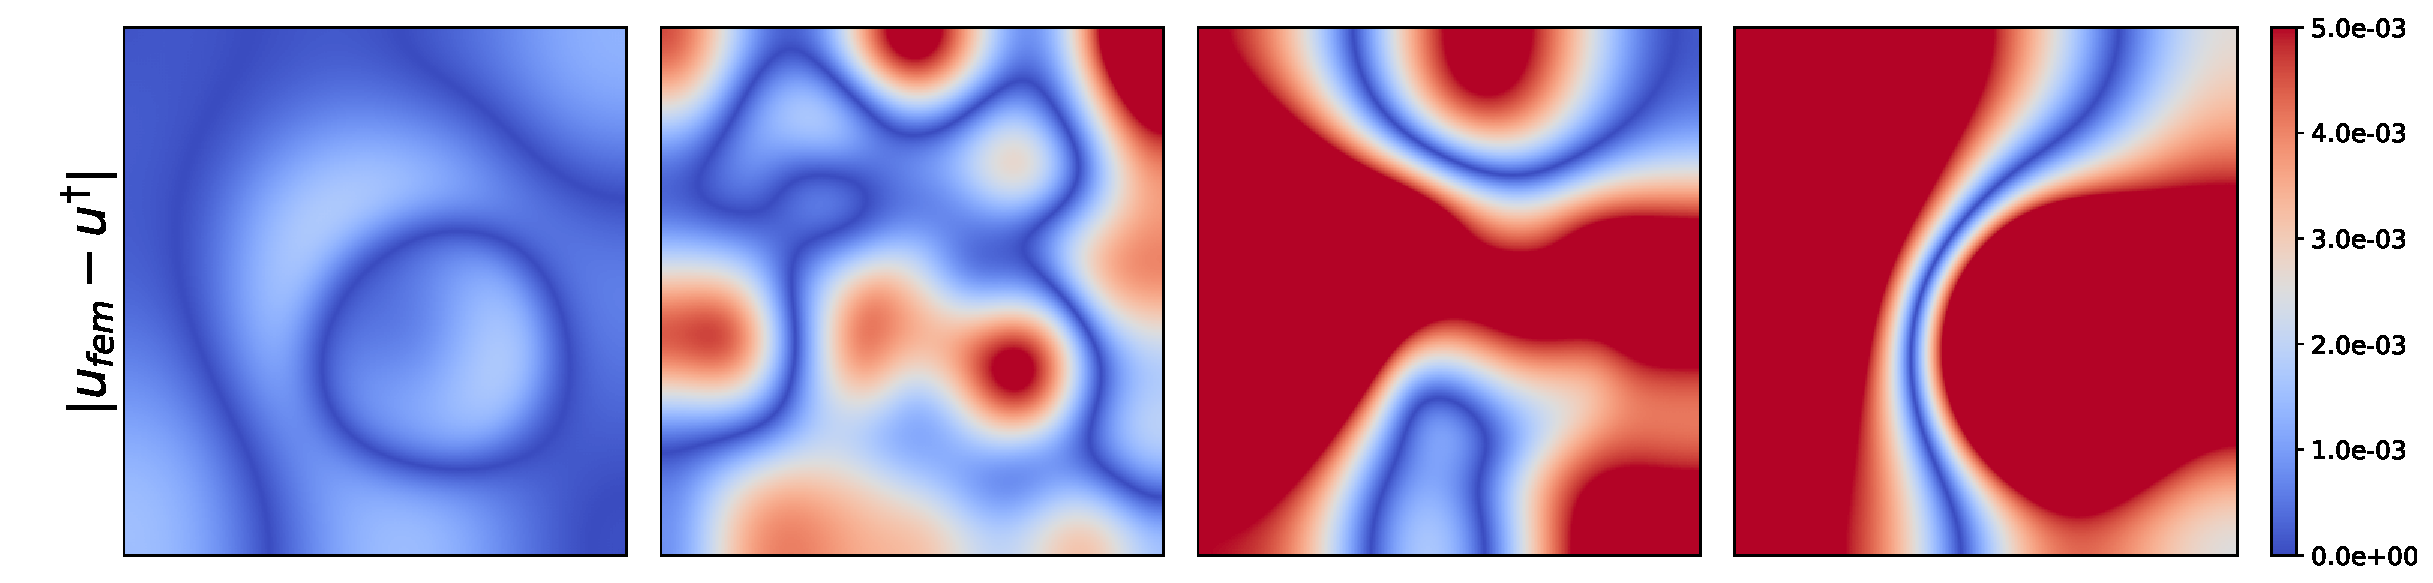
\includegraphics[width=\textwidth]{figures3/non_smooth_ufem_err.eps}
% \caption{从上到下依次为：Example \ref{example:nonsmooth} 中的真实势函数 $u^{\dagger}$，由 Tikhonov-PINNs 恢复的势函数 $u_{\text{pinn}}$，逐点绝对误差 $|u^{\dagger}-u_{\text{pinn}}|$，由 FEM 恢复的势函数 $u_{\text{fem}}$，逐点绝对误差 $|u^{\dagger}-u_{\text{fem}}|$。我们绘制了不同噪声水平下的结果。}
% \label{fig:example:nonsmooth:u}
% \end{figure}

% \begin{figure}[htbp]
% \centering
% \setlength{\abovecaptionskip}{10pt}
% 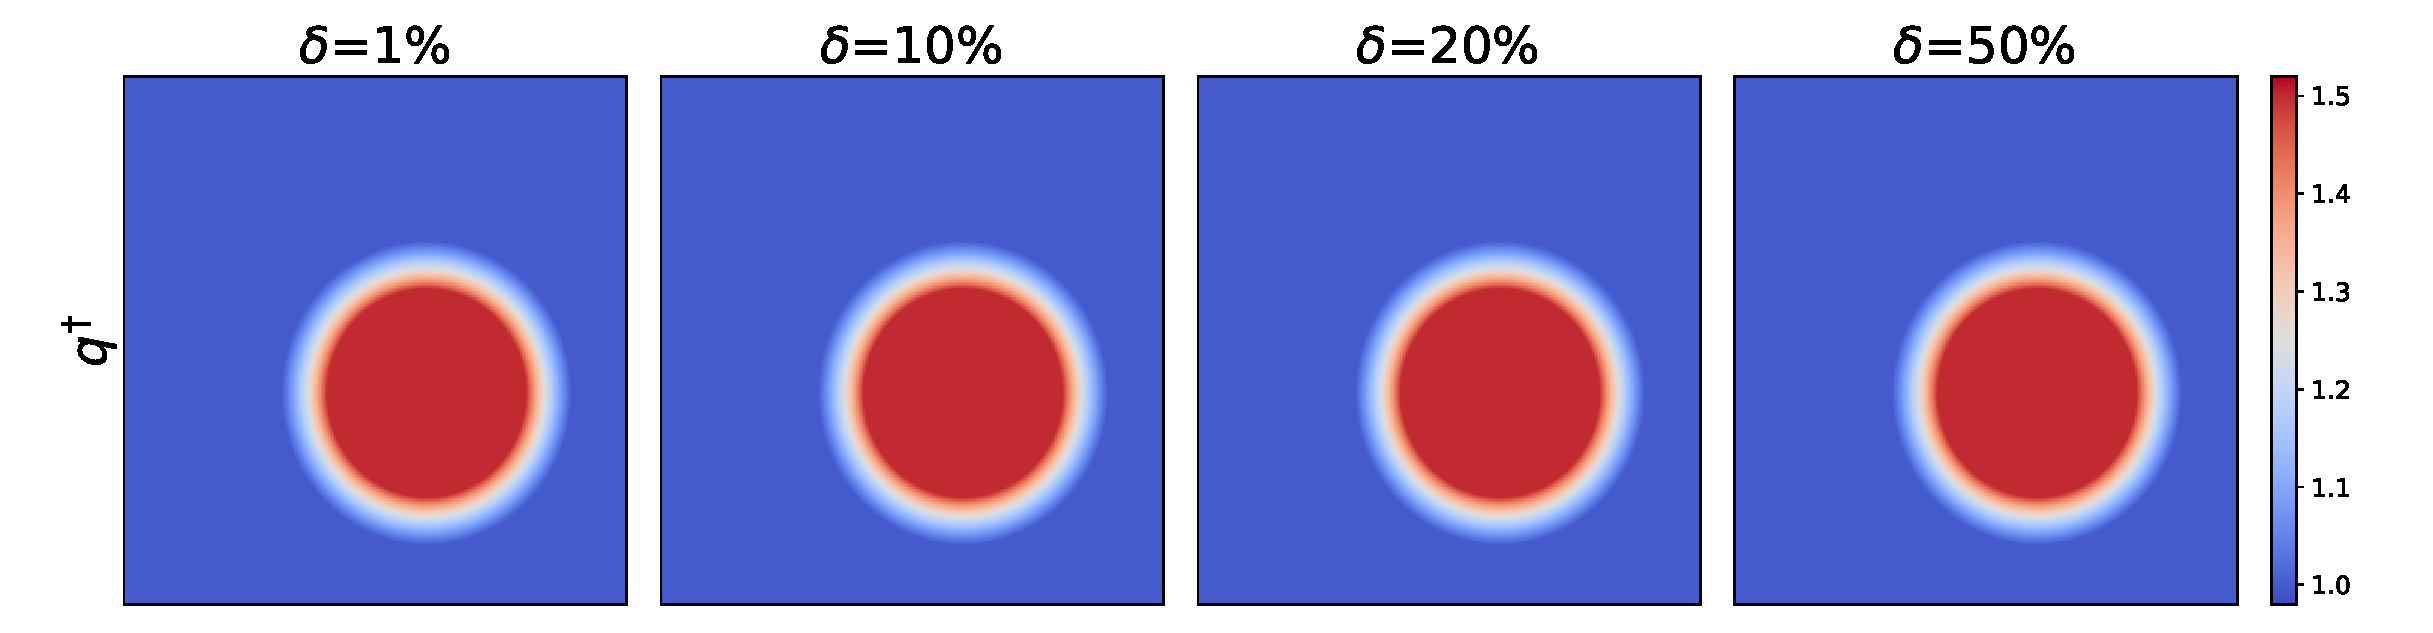
\includegraphics[width=\textwidth]{figures3/non_smooth_qdag.eps}\par
% 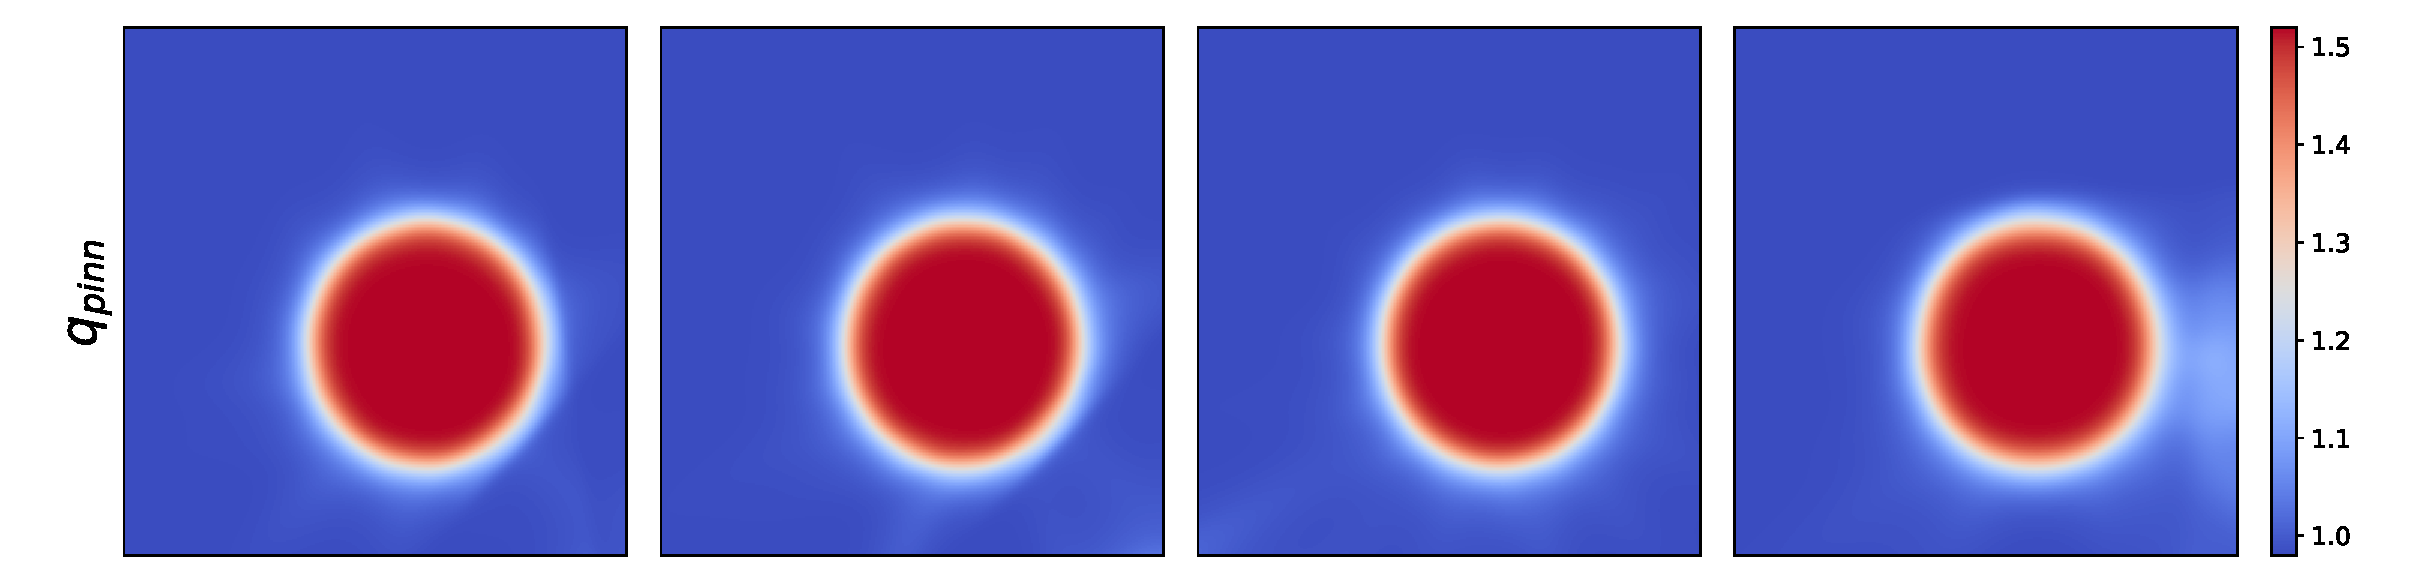
\includegraphics[width=\textwidth]{figures3/non_smooth_qnn.eps}\par
% 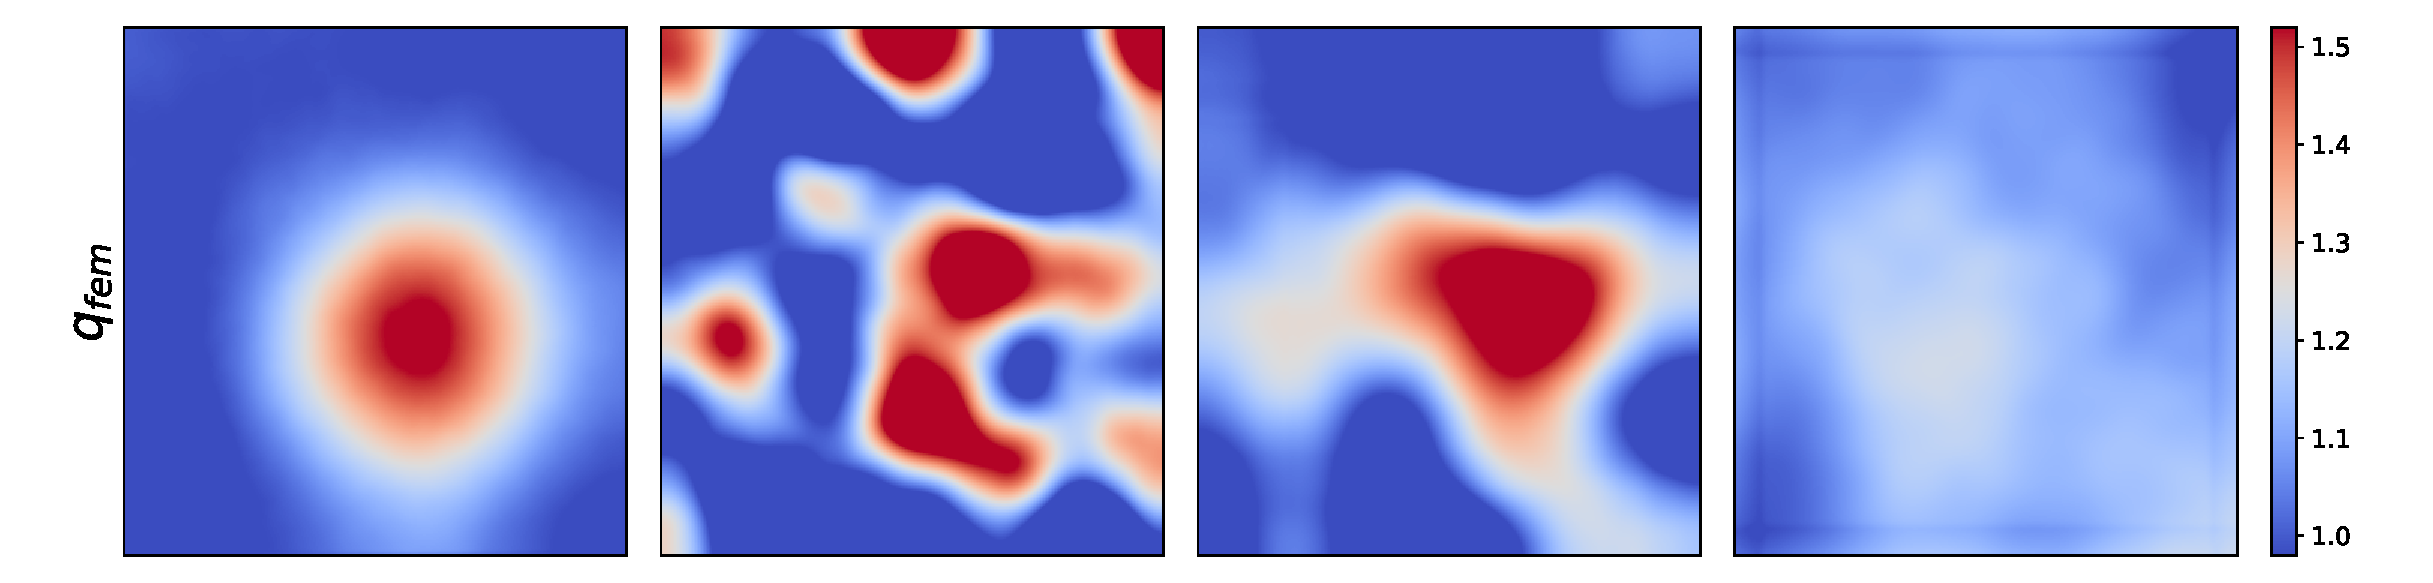
\includegraphics[width=\textwidth]{figures3/non_smooth_q_fem.eps}\par
% 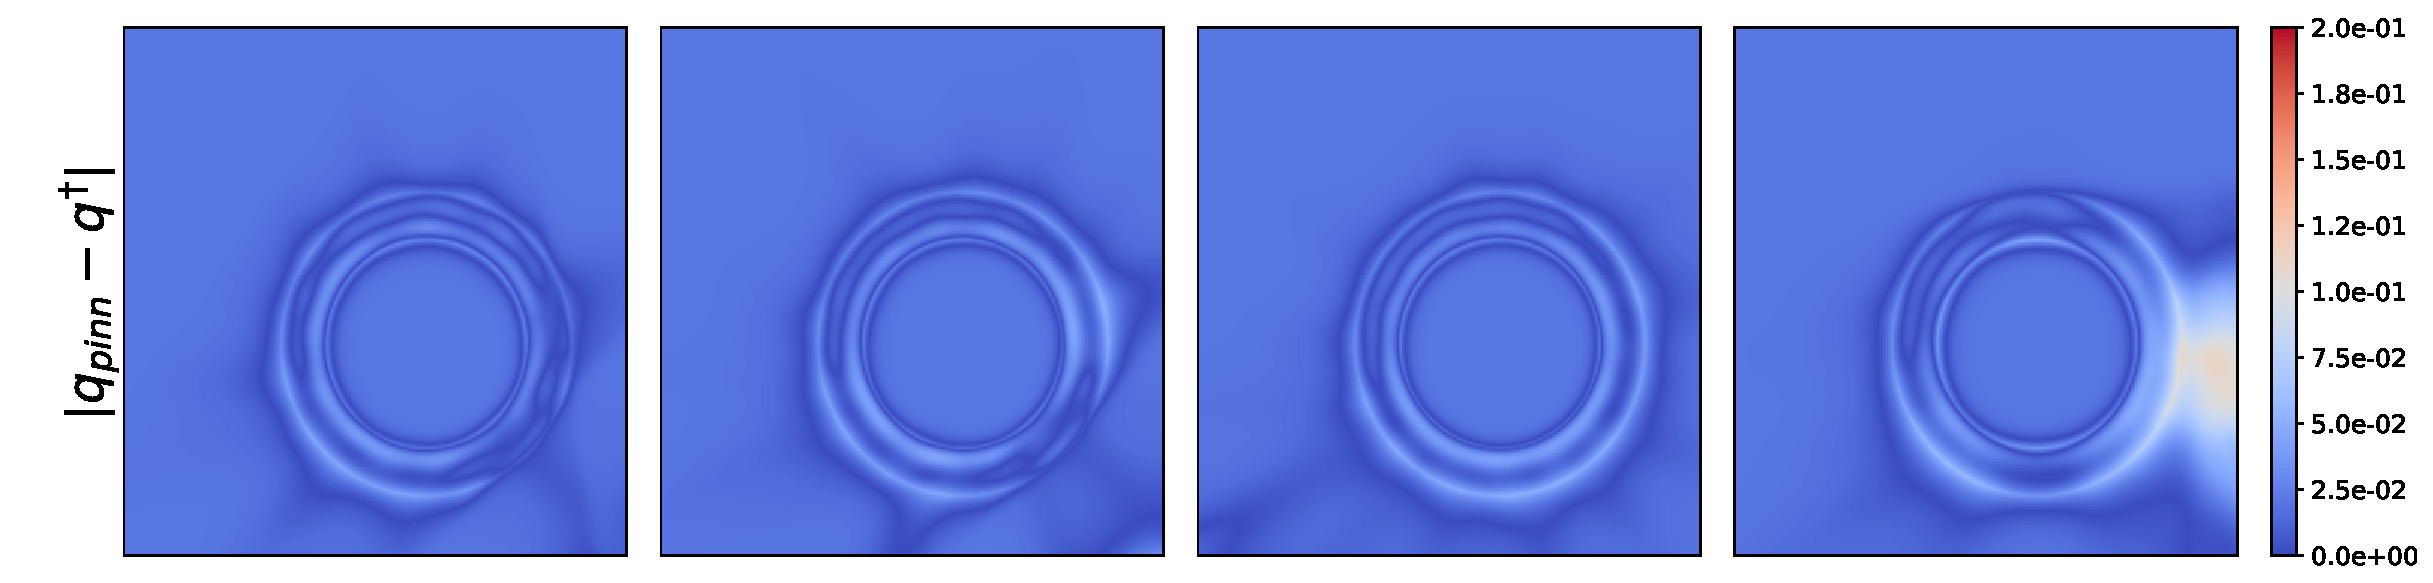
\includegraphics[width=\textwidth]{figures3/non_smooth_qnn_err.eps}\par
% 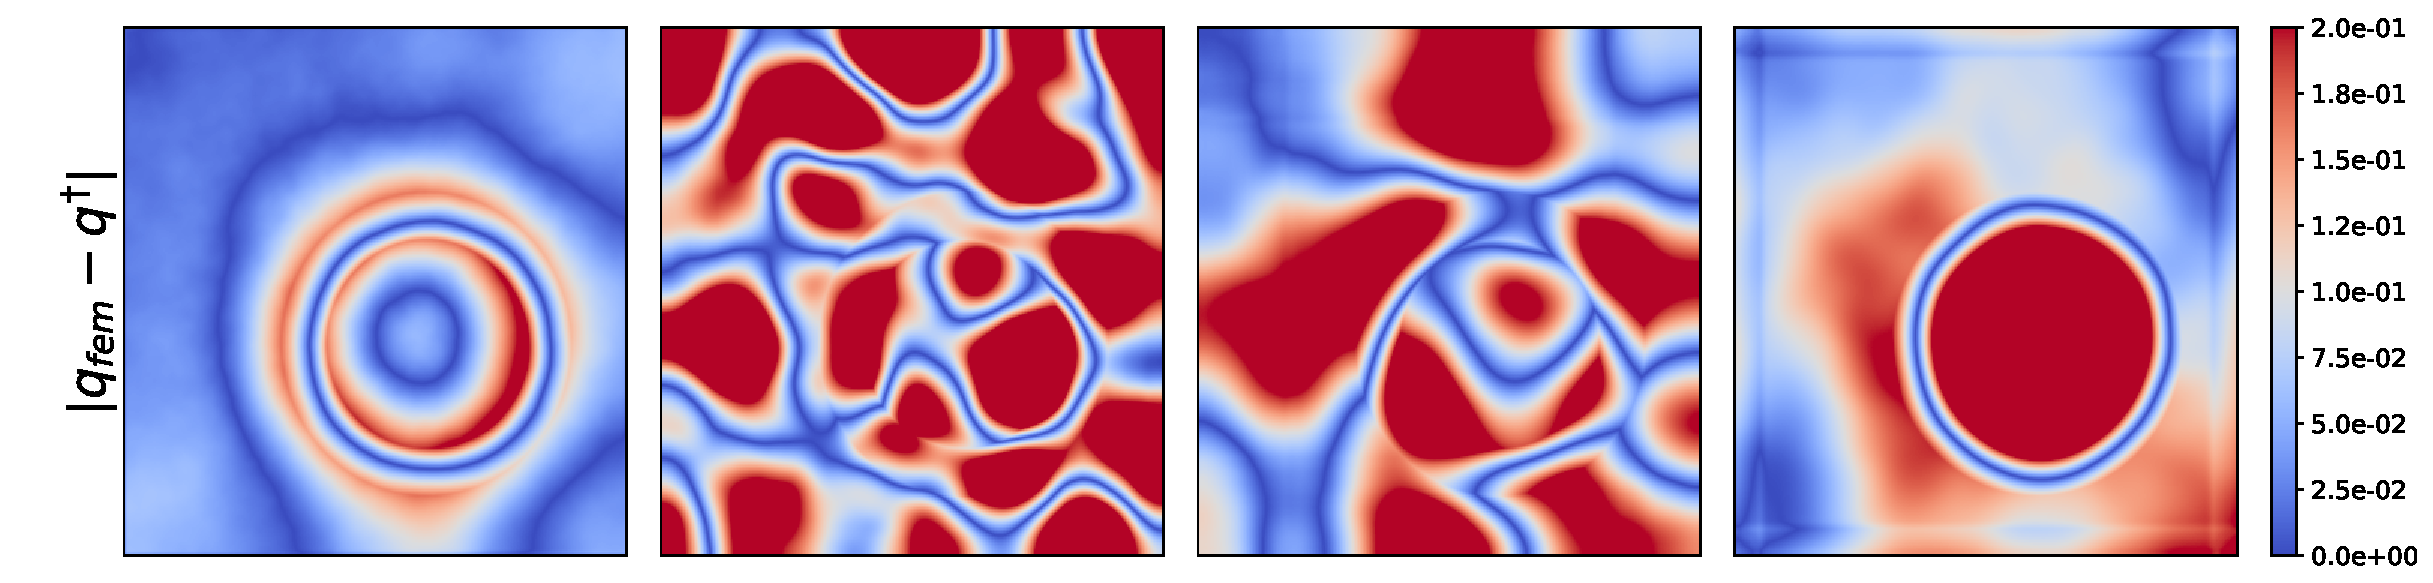
\includegraphics[width=\textwidth]{figures3/non_smooth_qfem_err.eps}
% \caption{从上到下依次为：Example \ref{example:nonsmooth} 中的真实势函数 $q^{\dagger}$，由 Tikhonov-PINNs 恢复的势函数 $q_{\text{pinn}}$，逐点绝对误差 $|q^{\dagger}-q_{\text{pinn}}|$，由 FEM 恢复的势函数 $q_{\text{fem}}$，逐点绝对误差 $|q^{\dagger}-q_{\text{fem}}|$。我们绘制了不同噪声水平下的结果。}
% \label{fig:example:nonsmooth}
% \end{figure}

% 在本例中，势函数 $q^{\dagger}$ 呈现出一种平台结构：它在红圈内部和蓝圈外部均保持常数。如图 \ref{fig:example:nonsmooth:u} 和图 \ref{fig:example:nonsmooth} 所示，重构 $u$ 相对简单，Tikhonov-PINNs 和基于有限元的方法均表现良好。然而，在重构 $q$ 时，Tikhonov-PINNs 成功捕捉到了常数值区域，而有限元方法未能精确识别 $q$ 中的界面，导致误差显著偏高。即使在高噪声水平下（例如 $\delta = 50\%$），我们的方法仍能恢复势函数的整体结构，而有限元方法几乎产生不了任何有意义的信息。

% \subsubsection{不连续问题}

% 作为第三个例子，我们将求解一个不连续势函数的反问题。
% \begin{example}\label{example:discontinuous}
% 令 $\Omega=(0,1)^{2}$ 且 $\alpha\equiv 1$。定义精确势函数 $q^{\dagger}$ 为：
% \begin{align*}
% \zeta(x_{1},x_{2})&=\exp\{-9\times(x_{1}-0.5)^{2}-9\times(x_{2}-0.5)^{2}\}, \\
% q^{\dagger}(x_{1},x_{2})&=1.0+0.5\times\zeta(x_{1},x_{2})\chi_{\{x_{1}\geq x_{2}\}},
% \end{align*}
% 精确解 $u^{\dagger}$ 为：$u^{\dagger}(x_{1},x_{2})=1+\sin(\pi x_{1})\sin(\pi x_{2})$。
% \end{example}

% \begin{table}[hbtp]
% \centering
% \footnotesize
% \caption{例 \ref{example:discontinuous} 中恢复的势函数 $\hat{q}$ 和解 $\hat{u}$ 的相对 $L^{2}$ 误差。}
% \begin{tabular}{lrrrrrr}
% \hline
% \multirow{2}[0]{*}{$\delta $ = 1\%} & \multicolumn{6}{c}{正则化参数 $\lambda$} \\
% \cline{2-7}
% & \multicolumn{1}{l}
% {$1.0\times 10^{-5}$} & 
% \multicolumn{1}{l}{$1.0\times 10^{-6}$} &
% \multicolumn{1}{l}{$1.0\times 10^{-7}$} &
% \multicolumn{1}{l}{$1.0\times 10^{-8}$} & 
%    \multicolumn{1}{l}{$1.0\times 10^{-9}$} & {0} \\
%    \hline
% $\text{err}(u_{\text{pinn}})$ & $2.05\times 10^{-3}$ & $1.54\times 10^{-3}$ & $1.07\times 10^{-3}$ & $9.83\times 10^{-4}$ & $7.55\times 10^{-4}$ & $6.42\times 10^{-4}$ \\
% $\text{err}(u_{\text{fem}})$&$1.46\times 10^{-3}$ & $7.05\times 10^{-4}$ & $4.80\times 10^{-4}$ & $2.66\times 10^{-4}$ & $2.50\times 10^{-4}$ & $2.38\times 10^{-4}$\\
% $\text{err}(q_{\text{pinn}})$ & $9.82\times 10^{-2}$ & $8.50\times 10^{-2}$ & $6.76\times 10^{-2}$ & $5.23\times 10^{-2}$ & $3.49\times 10^{-2}$ & \textbf{2.79$\times$ 10$^{-2}$} \\
% $\text{err}(q_{\text{fem}})$&$8.42\times 10^{-2}$ & $6.36\times 10^{-2}$ & $5.62\times 10^{-2}$ & $4.84\times 10^{-2}$ & $4.53\times 10^{-2}$ & $4.55\times 10^{-2}$\\
% \hline
% &       &       &       &       &       &  \\
% \hline
% \multirow{2}[0]{*}{$\delta$ = 10\%} & \multicolumn{6}{c}{正则化参数 $\lambda$} \\
% \cline{2-7}
% & $1.0\times 10^{-5}$ & $1.0\times 10^{-6}$ & $1.0\times 10^{-7}$ & $1.0\times 10^{-8}$ & $1.0\times 10^{-9}$ & \multicolumn{1}{r}{0} \\
% \hline
% $\text{err}(u_{\text{pinn}})$ & $1.96\times 10^{-3}$ & $1.74\times 10^{-3}$ & $1.38\times 10^{-3}$ & $1.12\times 10^{-3}$ & $1.49\times 10^{-3}$ & $1.48\times 10^{-3}$ \\
% $\text{err}(u_{\text{fem}})$&$1.80\times 10^{-3}$ & $9.42\times 10^{-4}$ & $1.42\times 10^{-3}$ & $1.53\times 10^{-3}$ & $1.69\times 10^{-3}$ & $1.97\times 10^{-3}$\\
% $\text{err}(q_{\text{pinn}})$ & $1.01\times 10^{-1}$ & $8.74\times 10^{-2}$ & $7.07\times 10^{-2}$ & \textbf{5.01$\times$ 10$^{-2}$} & $5.59\times 10^{-2}$ & $5.28\times 10^{-2}$ \\
% $\text{err}(q_{\text{fem}})$&$8.44\times 10^{-2}$ & $6.57\times 10^{-2}$ & $9.31\times 10^{-2}$ & $1.58\times 10^{-1}$ & $1.68\times 10^{-1}$ & $1.85\times 10^{-1}$\\
% \hline
% &       &       &       &       &       &  \\
% \hline
% \multirow{2}[0]{*}{$\delta = 20\%$} & \multicolumn{6}{c}{正则化参数 $\lambda$} \\
% \cline{2-7}
% & $1.0\times 10^{-5}$ & $1.0\times 10^{-6}$ & $1.0\times 10^{-7}$ & $1.0\times 10^{-8}$ & $1.0\times 10^{-9}$ & \multicolumn{1}{r}{0} \\
% \hline
% $\text{err}(u_{\text{pinn}})$ & $2.65\times 10^{-3}$ & $2.07\times 10^{-3}$ & $1.78\times 10^{-3}$ & $1.60\times 10^{-3}$ & $1.75\times 10^{-3}$ & $1.87\times 10^{-3}$ \\
% $\text{err}(u_{\text{fem}})$&$1.74\times 10^{-3}$ & $2.18\times 10^{-3}$ & $4.48\times 10^{-3}$ & $3.91\times 10^{-3}$ & $4.67\times 10^{-3}$ & $3.08\times 10^{-3}$\\
% $\text{err}(q_{\text{pinn}})$ & $1.05\times 10^{-1}$ & $9.18\times 10^{-2}$ & $7.22\times 10^{-2}$ & \textbf{6.50$\times$ 10$^{-2}$} & $7.20\times 10^{-2}$ & $7.73\times 10^{-2}$ \\
% $\text{err}(q_{\text{fem}})$&$8.58\times 10^{-2}$ & $9.39\times 10^{-2}$ & $2.35\times 10^{-1}$ & $2.00\times 10^{-1}$ & $6.43\times 10^{-1}$ & $1.89\times 10^{-1}$\\
% \hline
% &       &       &       &       &       &  \\
% \hline
% \multirow{2}[0]{*}{$\delta = 50\%$} & \multicolumn{6}{c}{正则化参数 $\lambda$} \\
% \cline{2-7}
% & $1.0\times 10^{-5}$ & $1.0\times 10^{-6}$ & $1.0\times 10^{-7}$ & $1.0\times 10^{-8}$ & $1.0\times 10^{-9}$ & \multicolumn{1}{r}{0} \\
% \hline
% $\text{err}(u_{\text{pinn}})$ & $3.92\times 10^{-3}$ & $4.57\times 10^{-3}$ & $4.33\times 10^{-3}$ & $4.23\times 10^{-3}$ & $4.21\times 10^{-3}$ & $4.35\times 10^{-3}$ \\
% $\text{err}(u_{\text{fem}})$&$4.99\times 10^{-3}$ & $7.18\times 10^{-3}$ & $8.53\times 10^{-3}$ & $8.25\times 10^{-3}$ & $1.29\times 10^{-2}$ & $1.01\times 10^{-2}$\\
% $\text{err}(q_{\text{pinn}})$ & $1.21\times 10^{-1}$ & $1.04\times 10^{-1}$ & $8.50\times 10^{-2}$ & $8.08\times 10^{-2}$ & \textbf{8.04$\times$ 10$^{-2}$} & $1.06\times 10^{-1}$ \\
% $\text{err}(q_{\text{fem}})$&$1.08\times 10^{-1}$ & $2.27\times 10^{-1}$ & $5.12\times 10^{-1}$ & $4.62\times 10^{-1}$ & $5.90\times 10^{-1}$ & $8.28\times 10^{-1}$\\
% \hline
% \end{tabular}
% \label{tab:discontinuous}
% \end{table}

% \begin{figure}[htbp]
% \centering
% \setlength{\abovecaptionskip}{10pt}
% 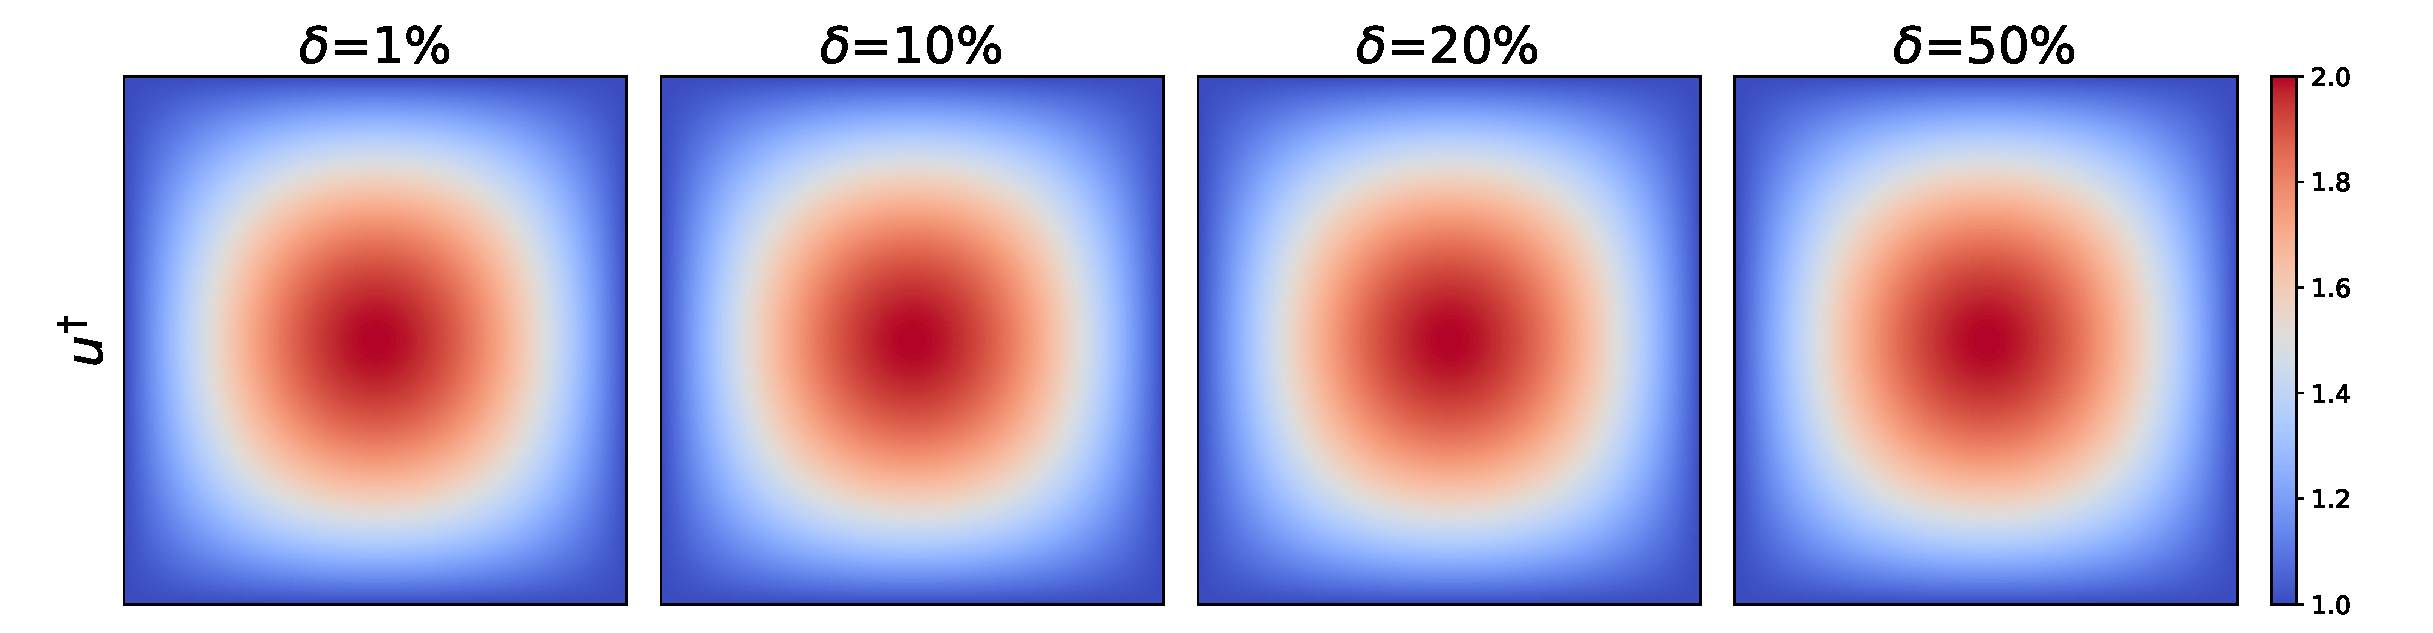
\includegraphics[width=\textwidth]{figures3/discontinuous_udag.eps}\par
% 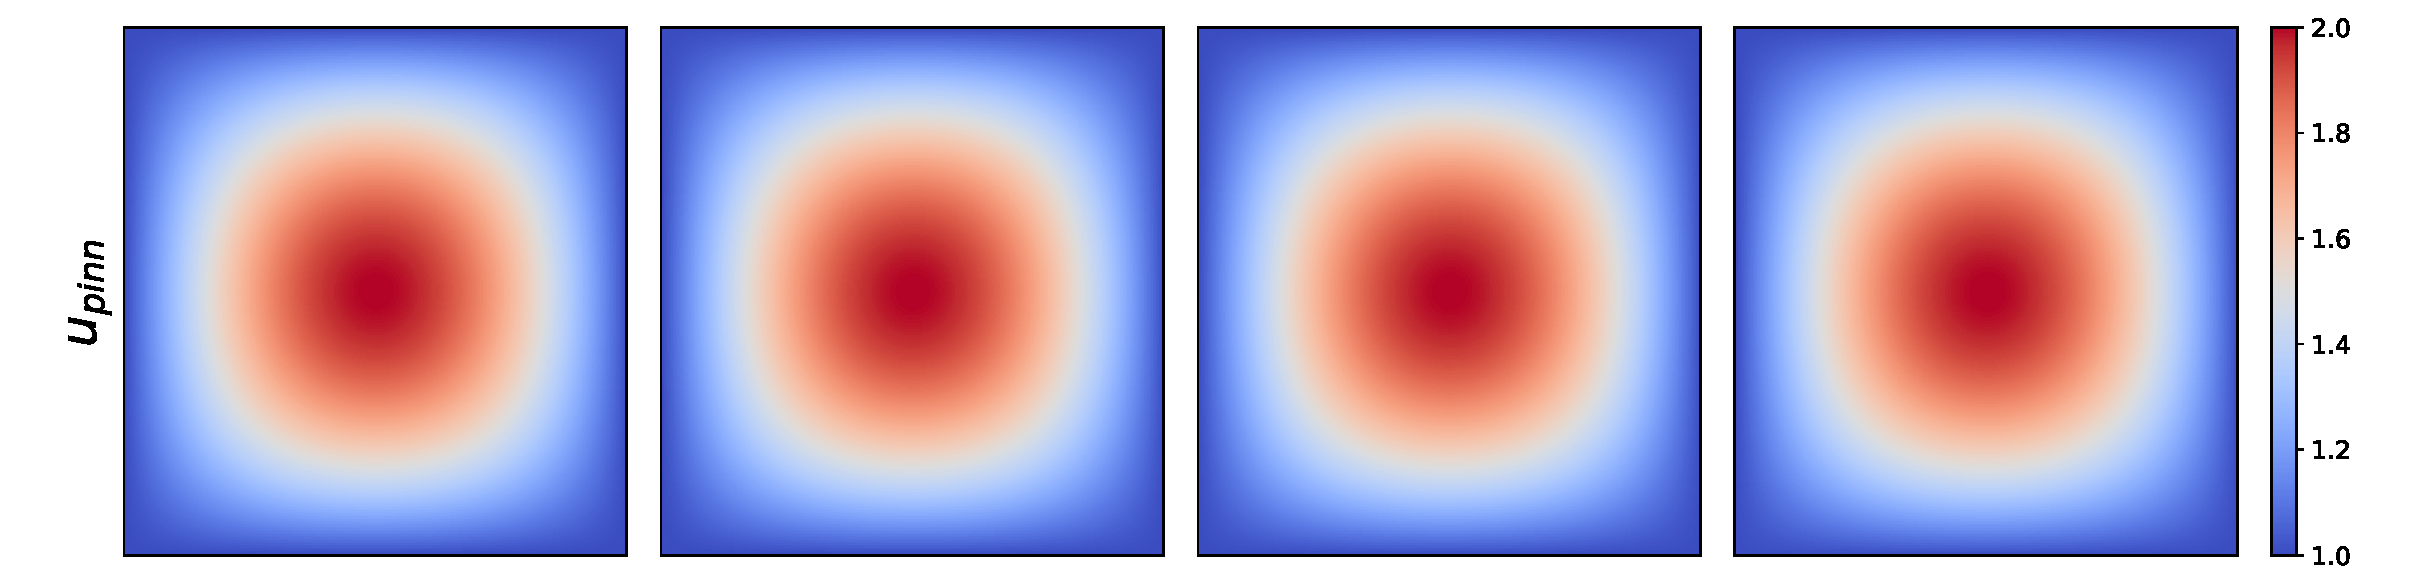
\includegraphics[width=\textwidth]{figures3/discontinuous_unn.eps}\par
% 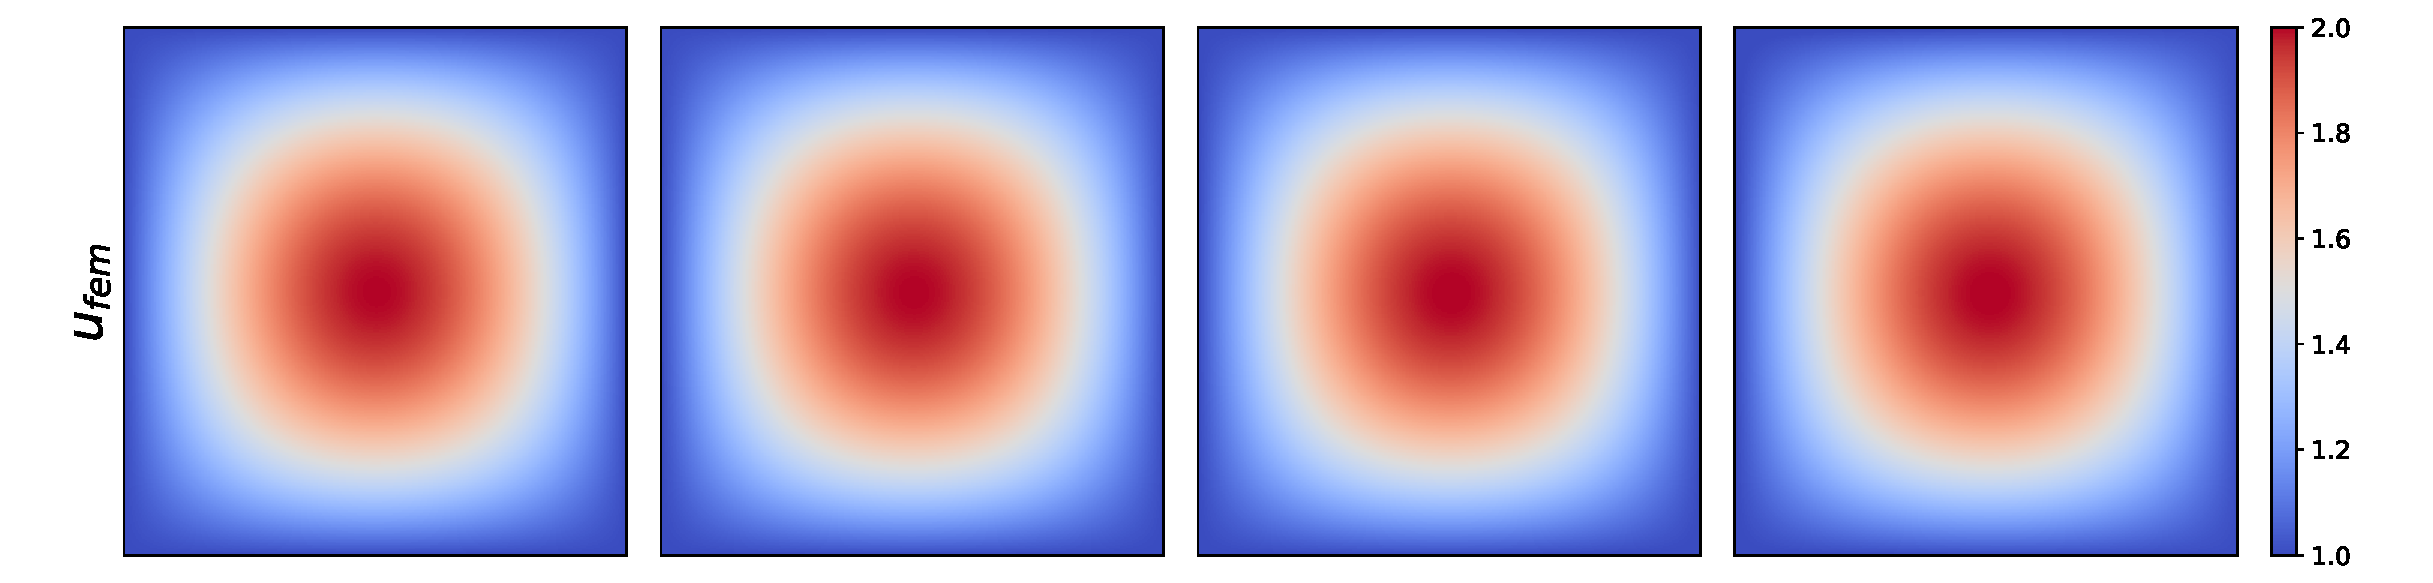
\includegraphics[width=\textwidth]{figures3/discontinuous_ufem.eps}\par
% 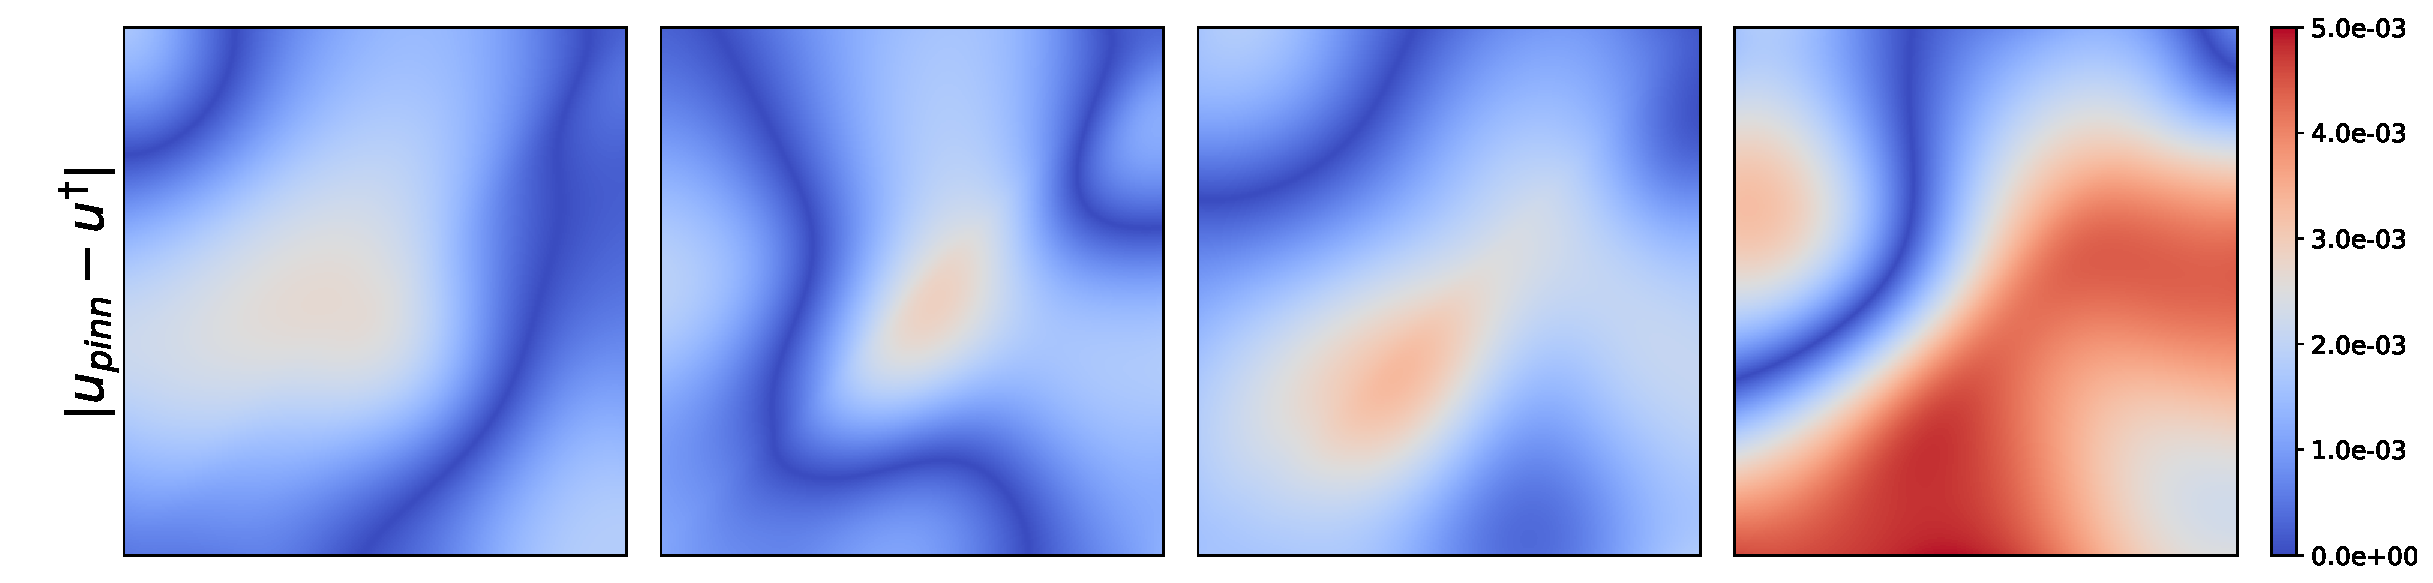
\includegraphics[width=\textwidth]{figures3/discontinuous_unn_err.eps}\par
% 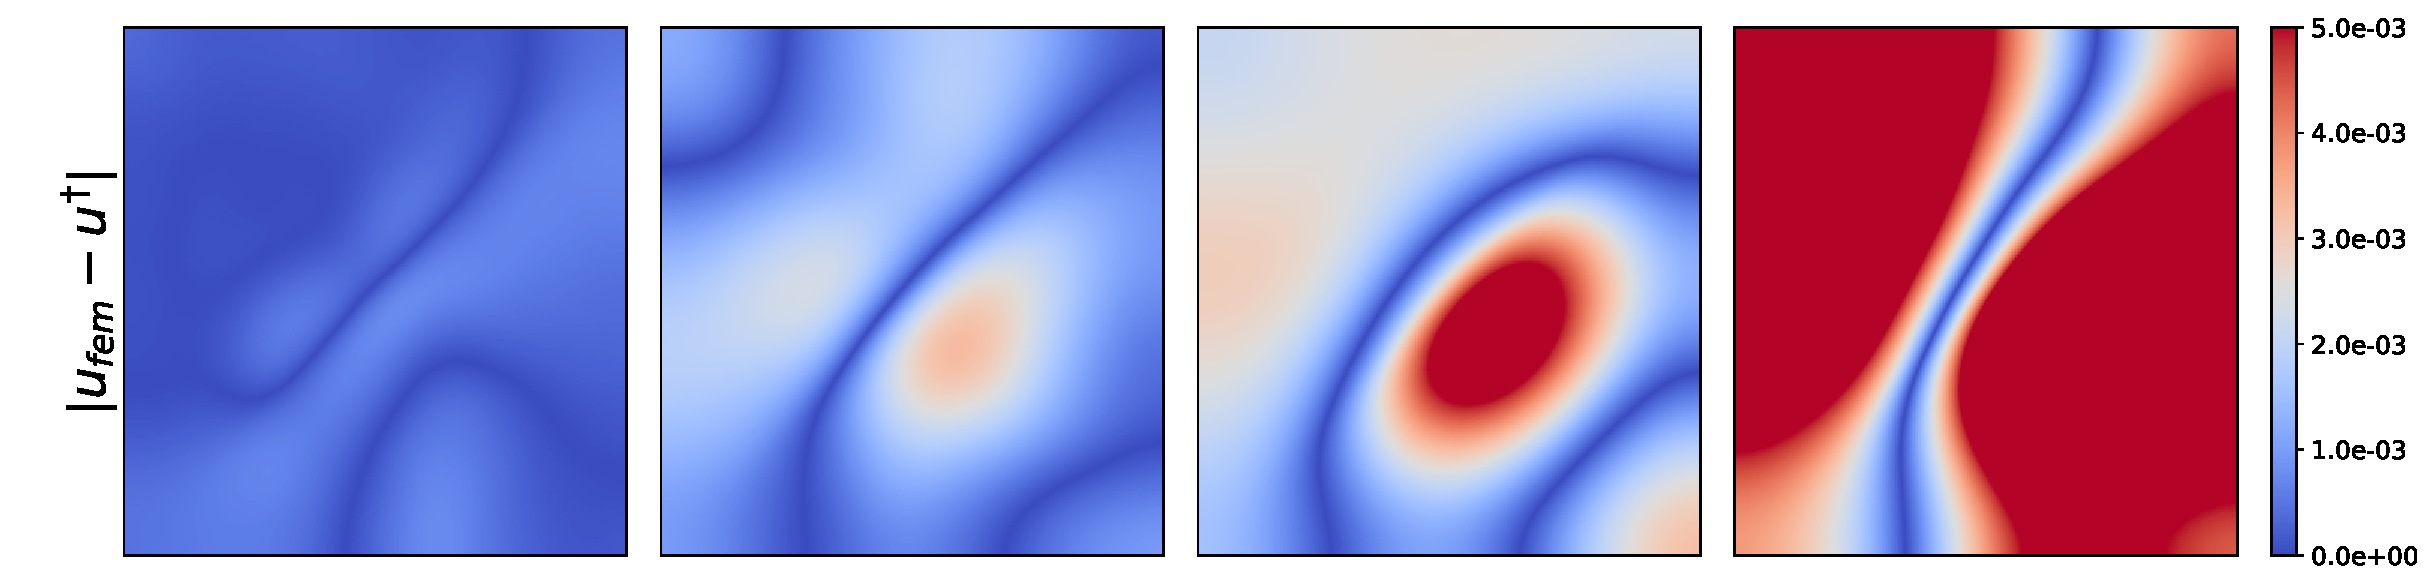
\includegraphics[width=\textwidth]{figures3/discontinuous_ufem_err.eps}
% \caption{从上到下依次为：例 \ref{example:discontinuous} 中的真实解 $u^{\dagger}$，Tikhonov-PINNs 恢复的解 $u_{\text{pinn}}$，逐点绝对误差 $|u^{\dagger}-u_{\text{pinn}}|$，FEM 恢复的解 $u_{\text{fem}}$，以及逐点绝对误差 $|u^{\dagger}-u_{\text{fem}}|$。我们绘制了在不同噪声水平下的结果。}
% \label{fig:example:discontinuous:u}
% \end{figure}

% \begin{figure}[htbp]
% \centering
% \setlength{\abovecaptionskip}{10pt}
% 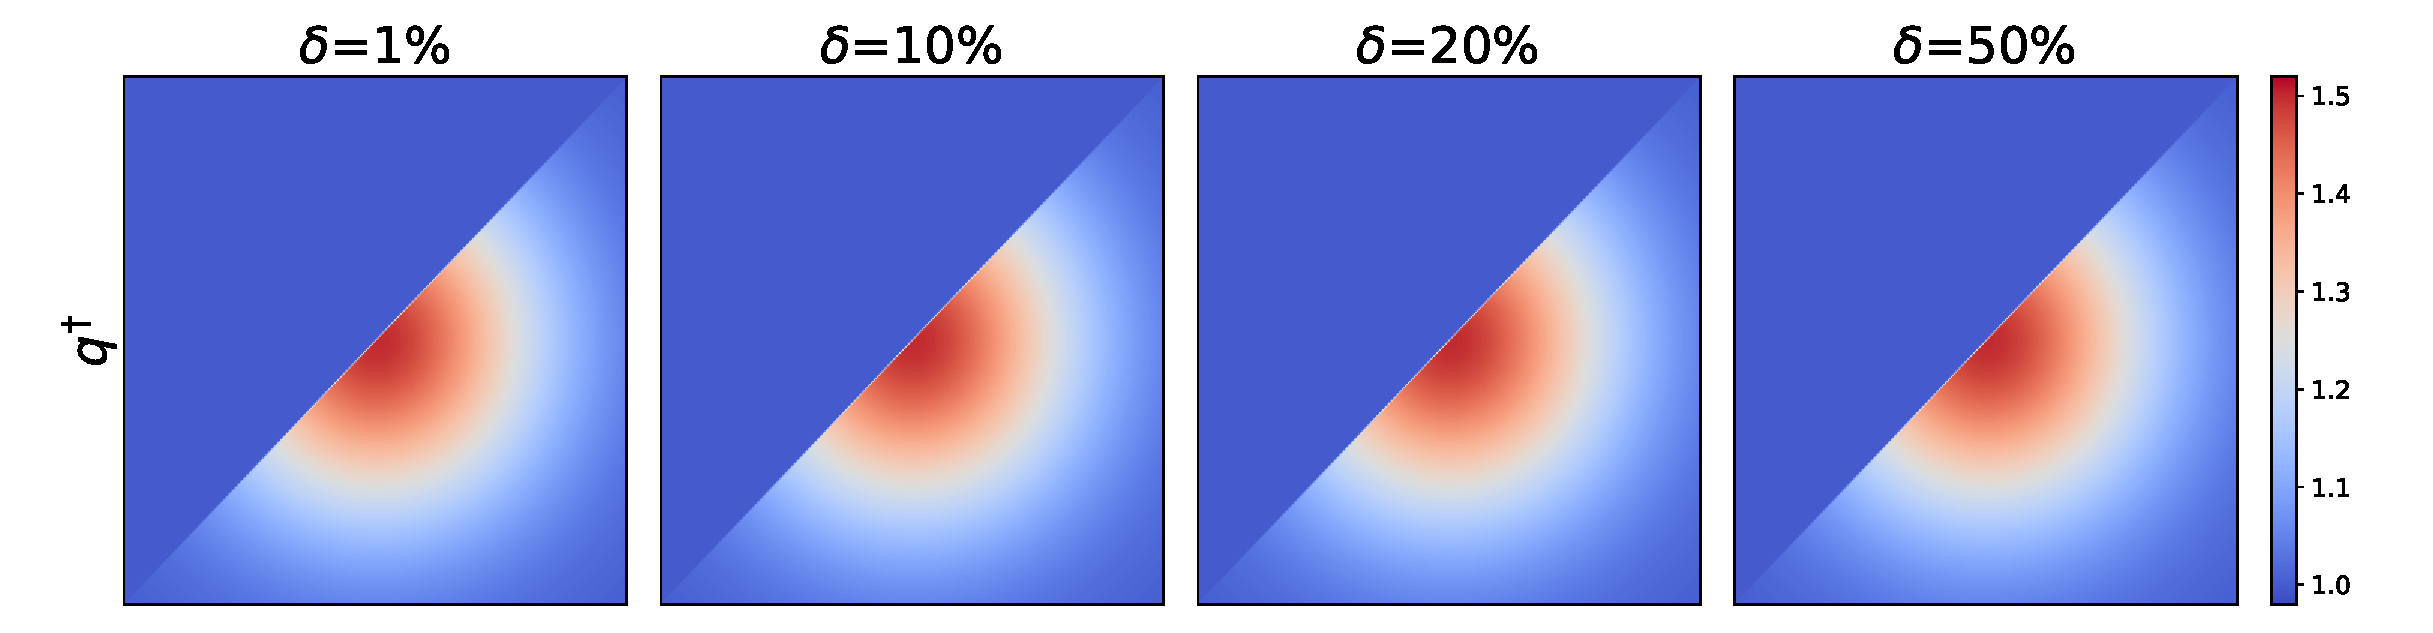
\includegraphics[width=\textwidth]{figures3/discontinuous_qdag.eps}\par
% 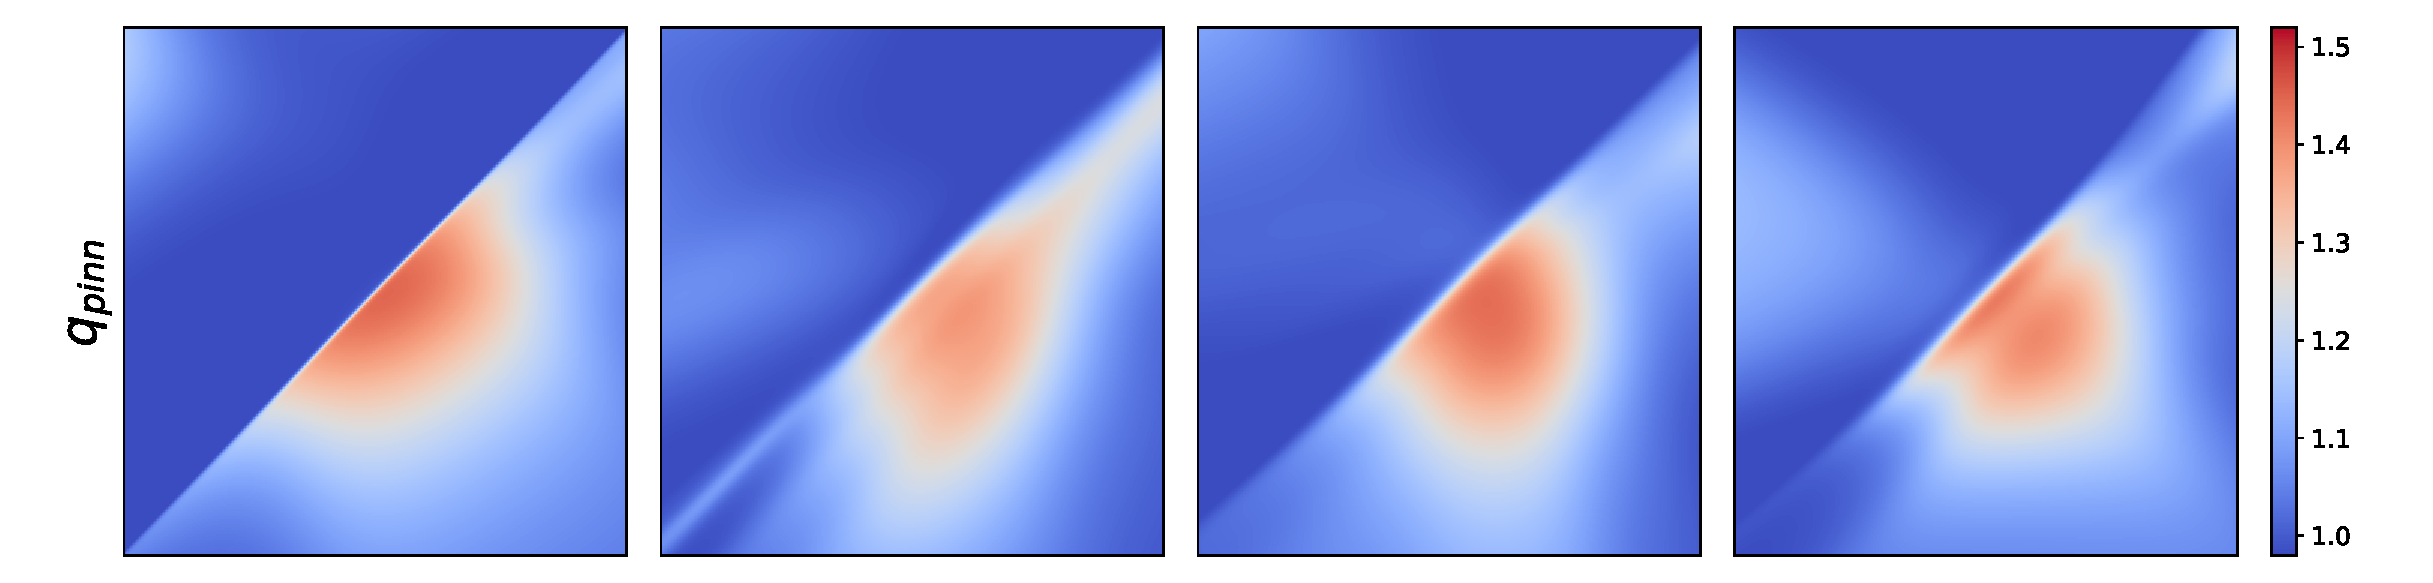
\includegraphics[width=\textwidth]{figures3/discontinuous_qnn.eps}\par
% 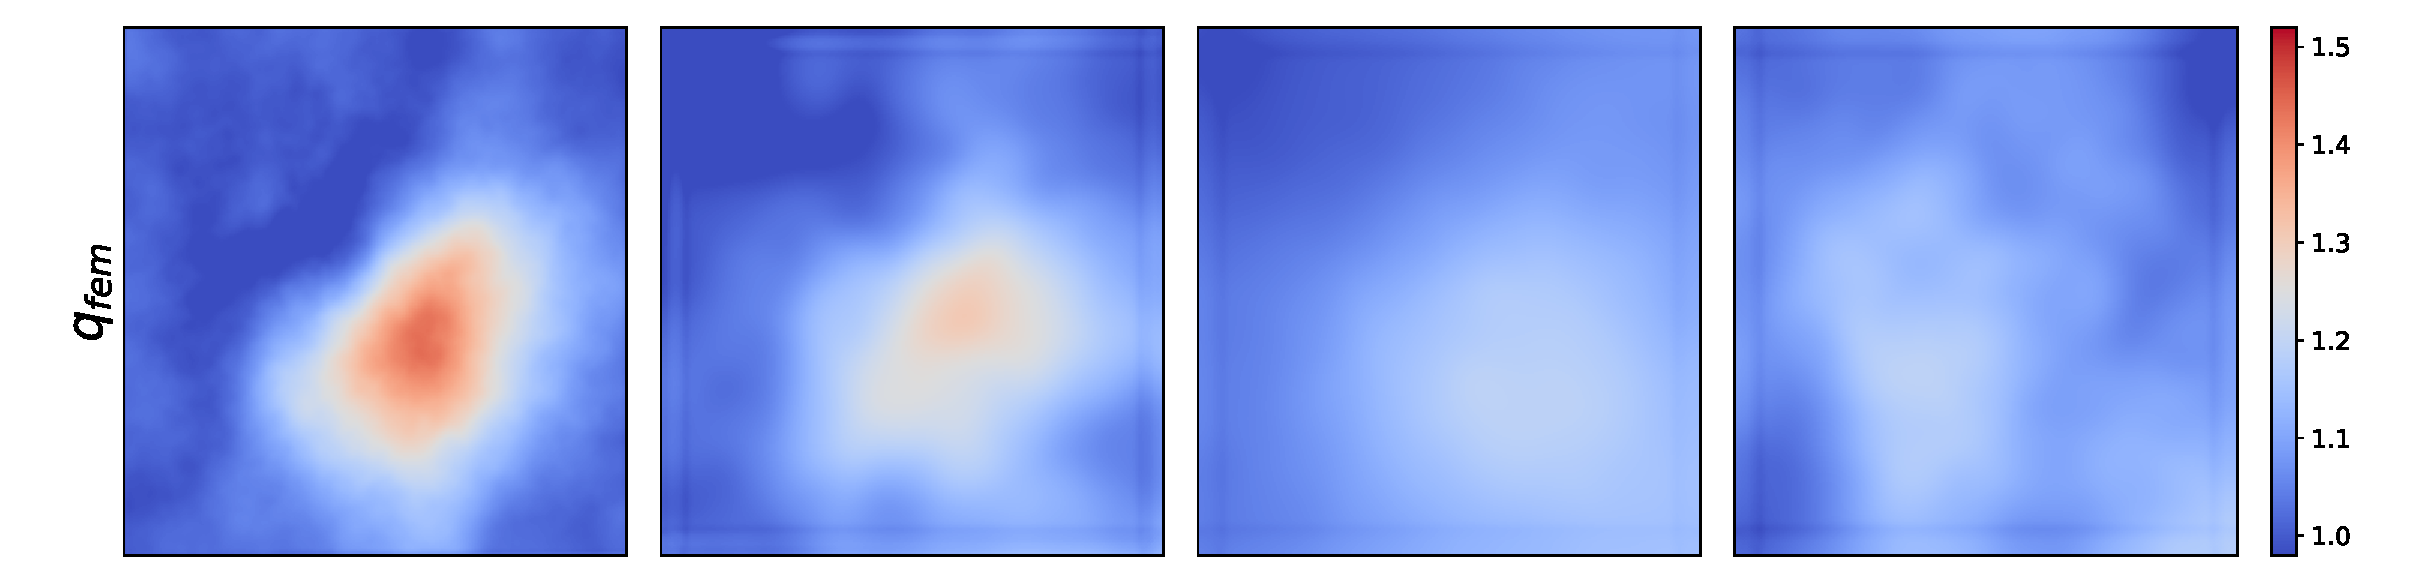
\includegraphics[width=\textwidth]{figures3/discontinuous_q_fem.eps}\par
% 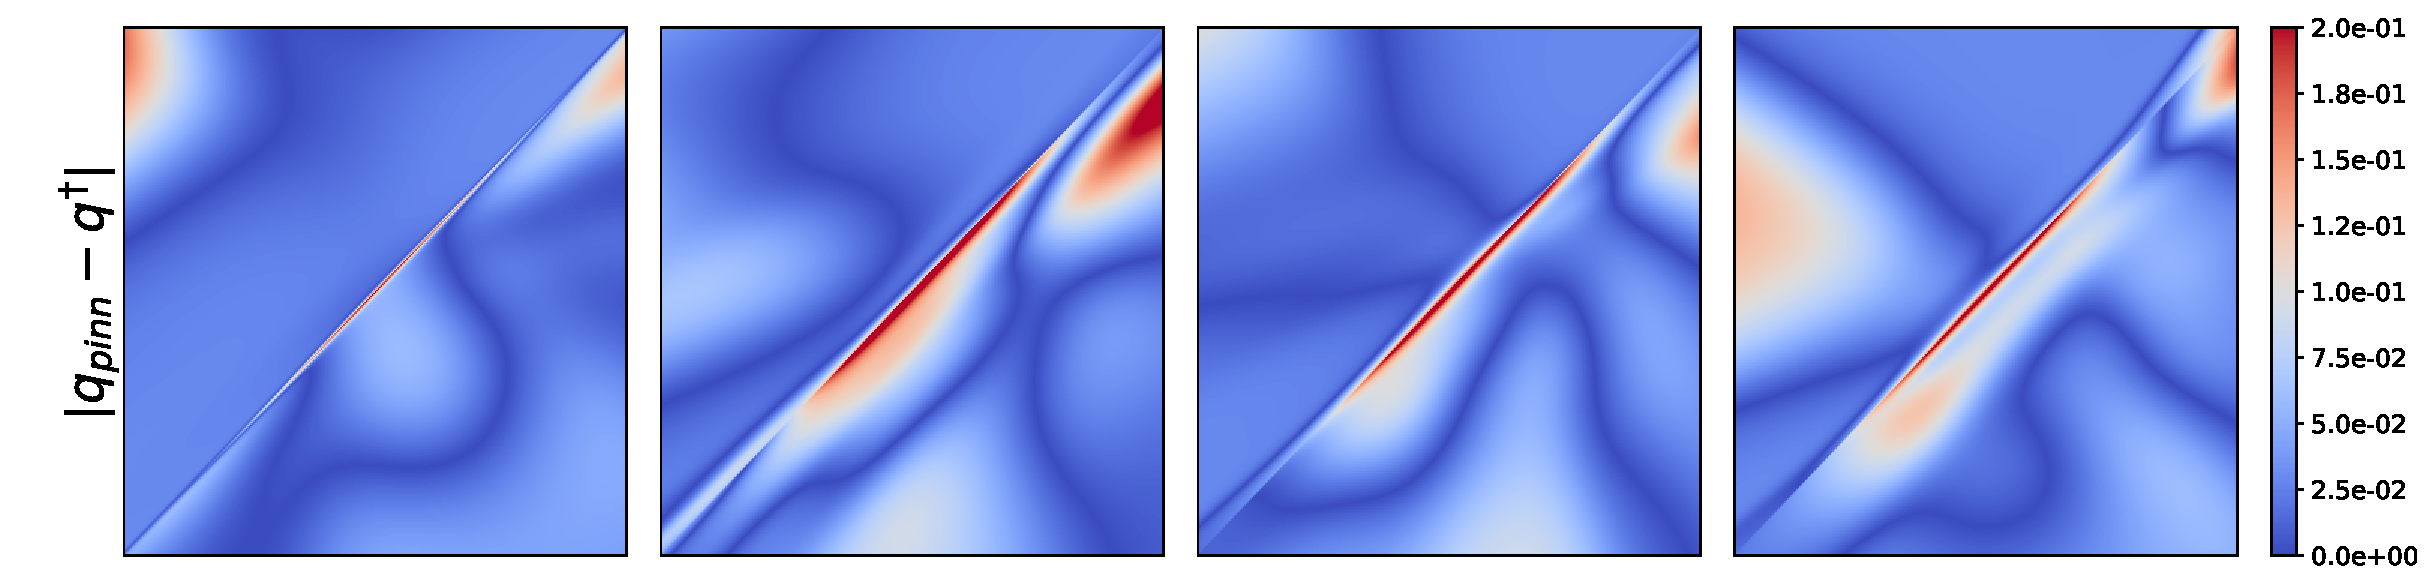
\includegraphics[width=\textwidth]{figures3/discontinuous_qnn_err.eps}\par
% 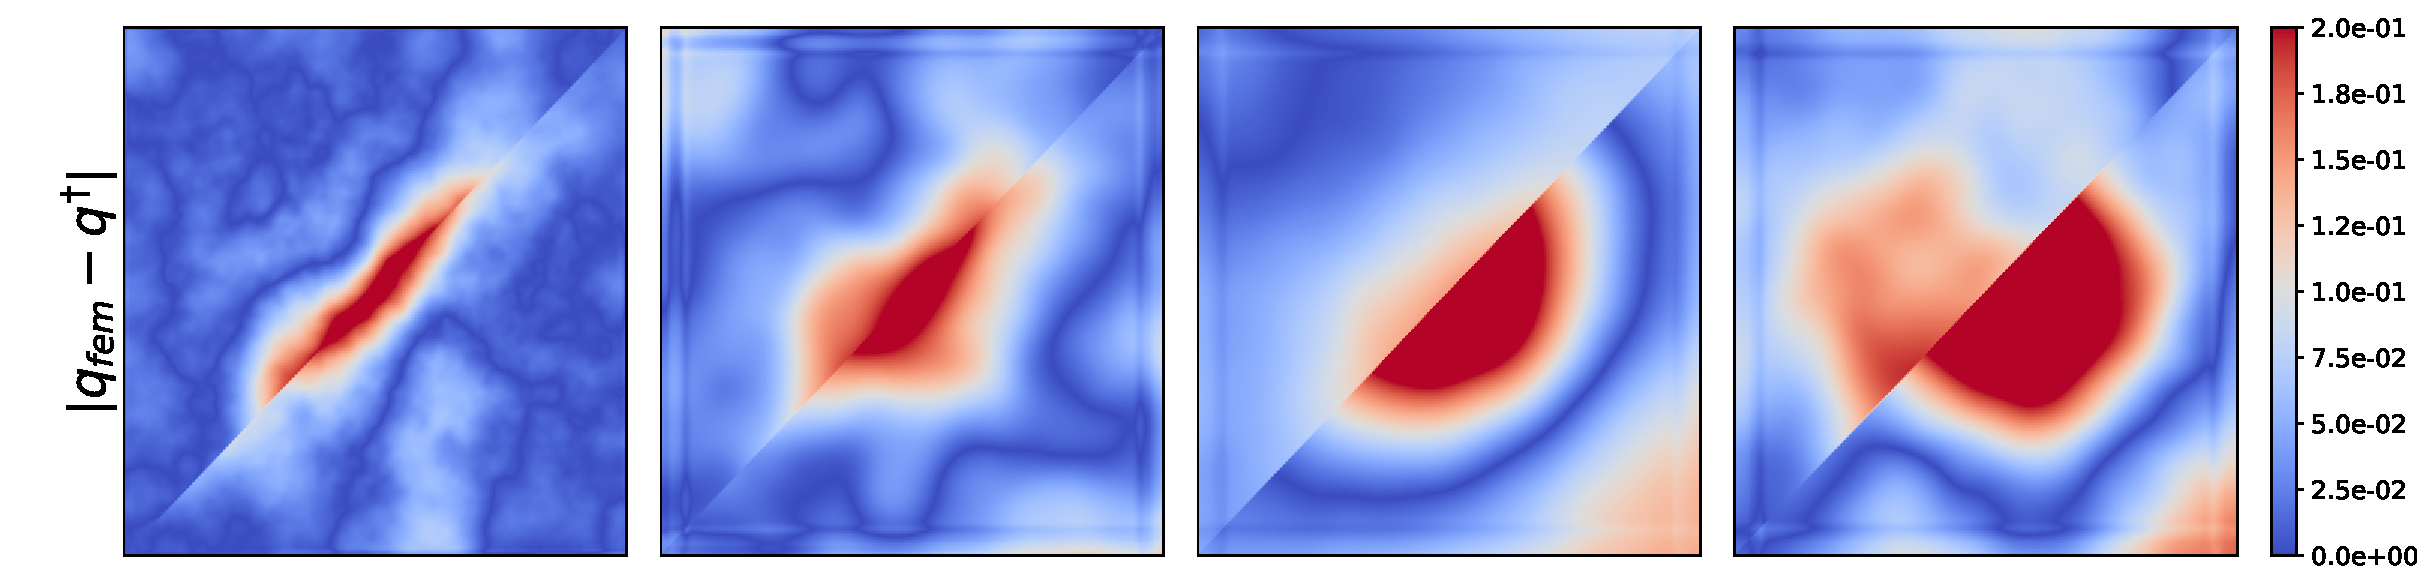
\includegraphics[width=\textwidth]{figures3/discontinuous_qfem_err.eps}
% \caption{从上到下依次为：例 \ref{example:discontinuous} 中的真实势函数 $q^{\dagger}$，Tikhonov-PINNs 恢复的势函数 $q_{\text{pinn}}$，逐点绝对误差 $|q^{\dagger}-q_{\text{pinn}}|$，FEM 恢复的势函数 $q_{\text{fem}}$，以及逐点绝对误差 $|q^{\dagger}-q_{\text{fem}}|$。我们绘制了在不同噪声水平下的结果。}
% \label{fig:example:discontinuous}
% \end{figure}

% 根据构造，势函数 $q$ 沿对角线 $x=y$ 呈现不连续性，这进一步加剧了反问题的不适定性。如图~\ref{fig:example:discontinuous:u} 和图~\ref{fig:example:discontinuous} 所示，Tikhonov-PINNs 能够在所有噪声水平下捕捉到这种不连续性。相比之下，有限元方法无法识别不连续区域，仅能在 1\% 的噪声水平下粗略定位高势区域。如表 \ref{tab:discontinuous} 所示，Tikhonov-PINNs 在所有噪声水平下对 $q$ 的相对误差均达到 $\calO(10^{-2})$ 左右，通常比有限元方法优越一个数量级。

% 还应注意，在上述实验中，当 $\lambda$ 非零时，Tikhonov-PINNs 通常能获得最优解（参见表 \ref{tab:discontinuous}）。这一观察结果部分说明了损失函数中的 Tikhonov 正则化对于提升标准 PINNs 方法的性能至关重要。

% \subsection{高维问题}
% 由于其无网格的特性，基于神经网络的方法可以很容易地扩展到高维问题，并在一定程度上缓解维数灾难。在本小节中，依照 \cite{jin2023conductivity} 中算例 5.4 的设置，我们将 Tikhonov-PINNs 应用于一个五维问题，这是传统有限元方法难以实现的场景。

% \begin{example}\label{example:highdim}
% 令 $\Omega=(0,1)^{5}$ 且 $\alpha\equiv 1$。我们考虑识别如下势函数：
% \begin{equation*}
% \begin{array}{rcl}
% q^{\dagger}(x)&=&1-(x_1-0.5)^2-(x_2-0.5)^2\\
% &{}&+\cos(\pi(x_3+1.5))+\cos(\pi (x_4+1.5))+\cos(\pi (x_5+1.5)),
% \end{array}
% \end{equation*}
% 准确解 $u^{\dagger}$ 为 $u^{\dagger}(x)=\sum_{i=1}^{5}(x_{i}+\frac{1}{3}x_{i}^3)$。
% \end{example}


% \begin{figure}
% \centering
% \setlength{\abovecaptionskip}{10pt}
% 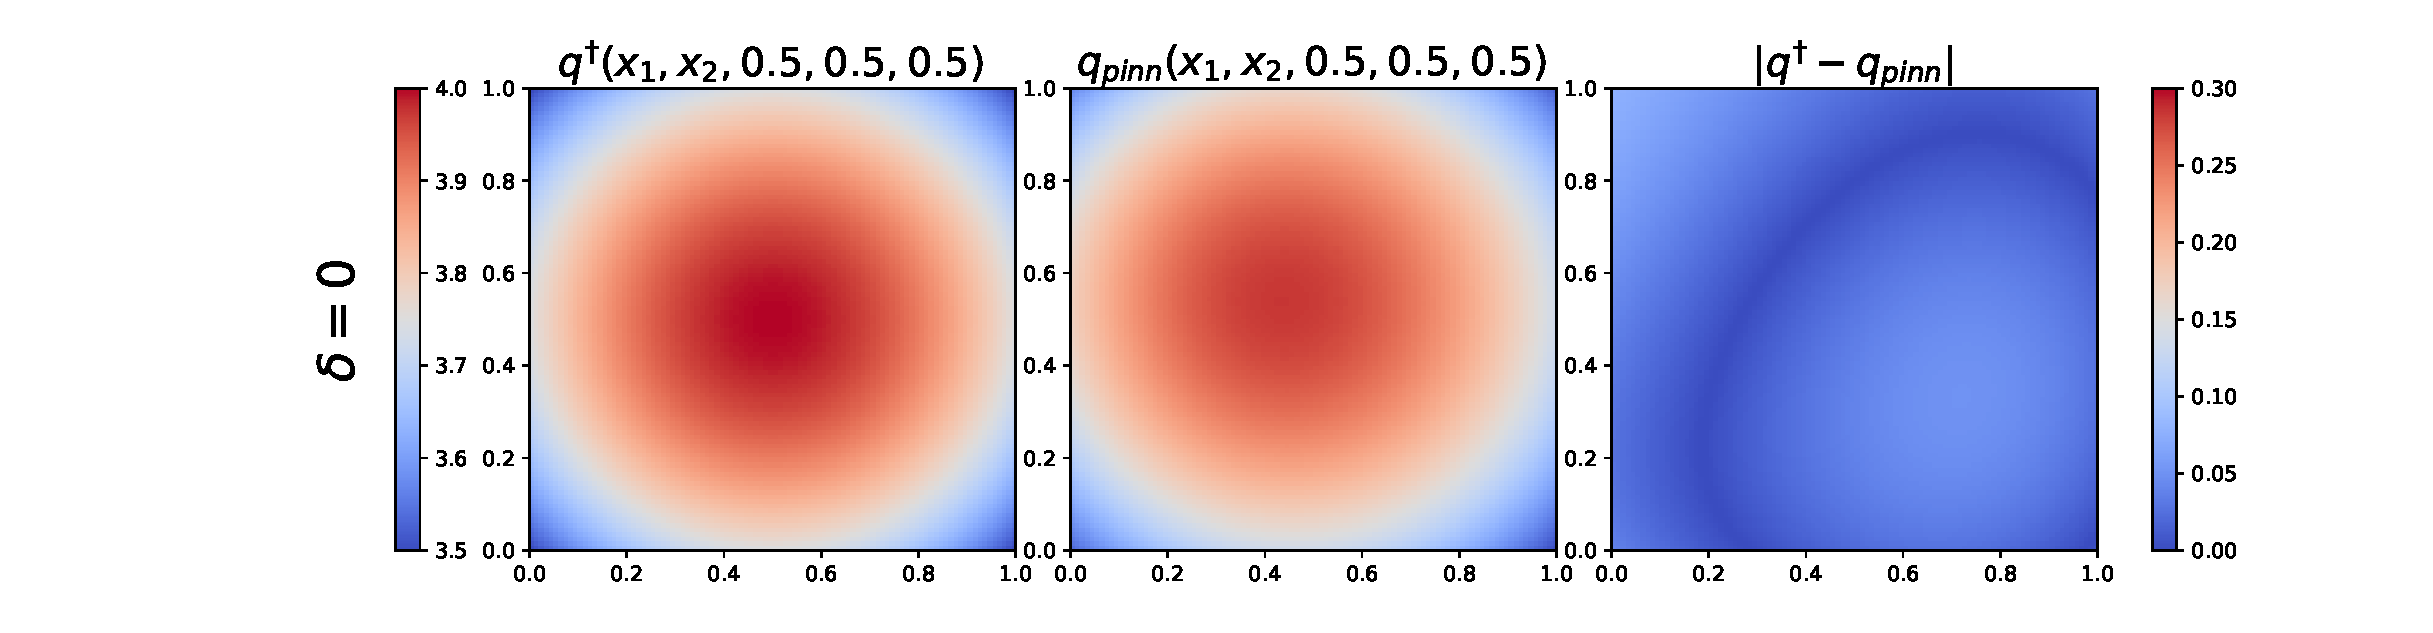
\includegraphics[width=\textwidth]{figures3/ex_5_00.eps}\par
% 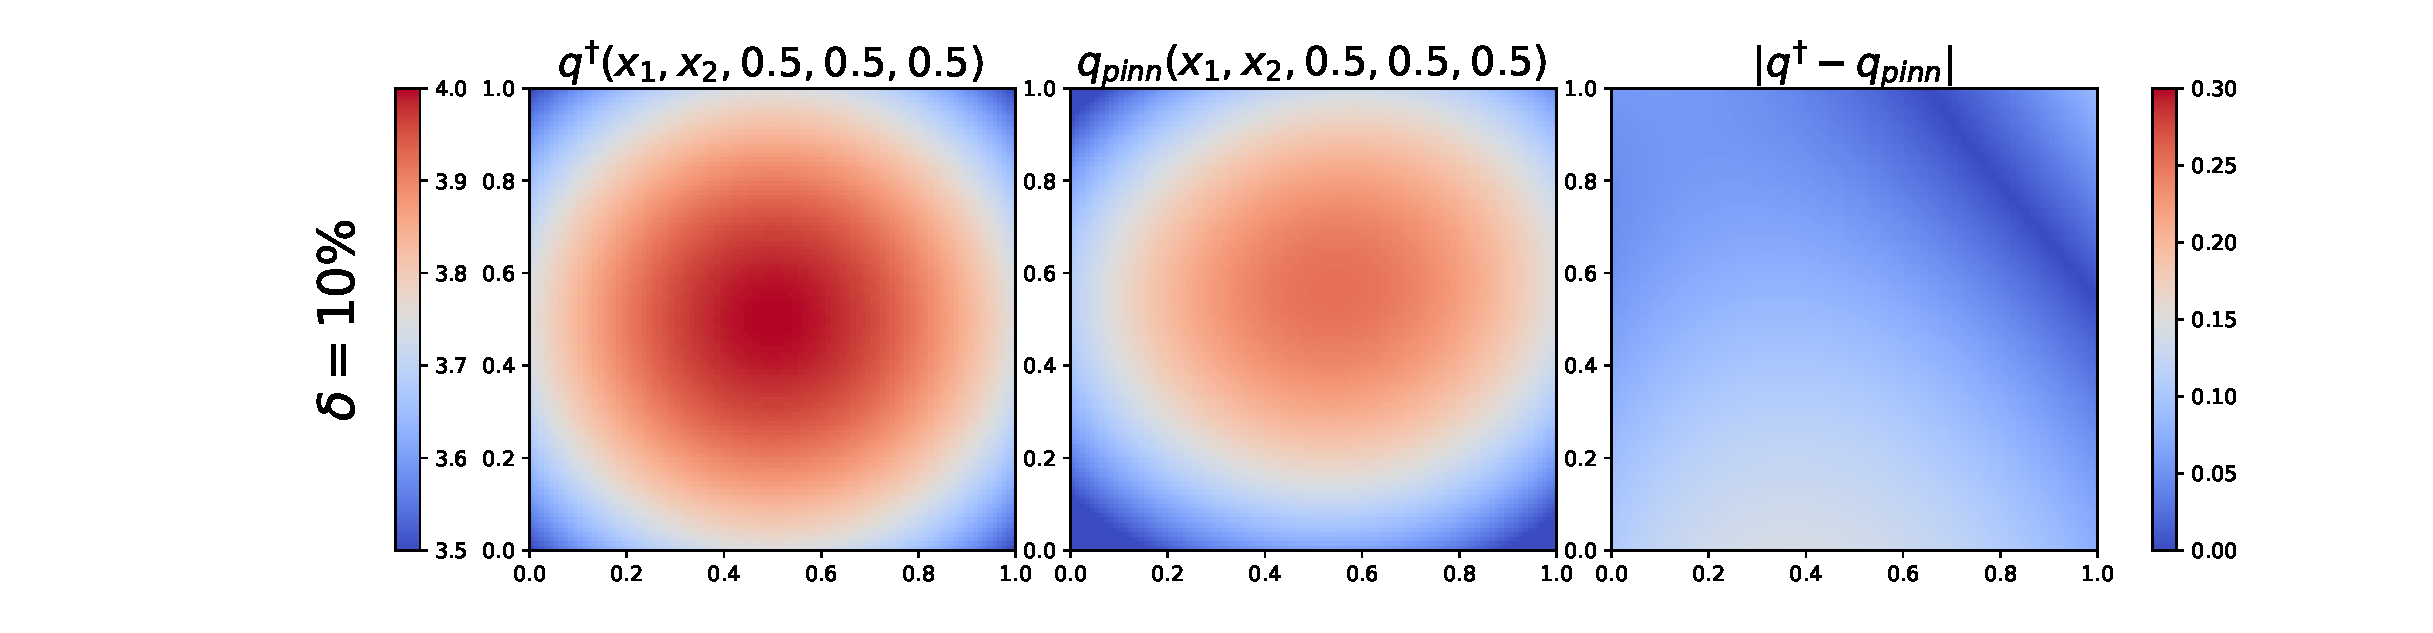
\includegraphics[width=\textwidth]{figures3/ex_5_10.eps}\par
% \caption{算例 \ref{example:highdim} 在切片 $x_3=x_4=x_5=0.5$ 上的真实解与 Tikhonov-PINNs 解。第一行对应 $\delta=0$ 的情况，而第二行展示了 $\delta=10\%$ 的情况。}
% \label{fig:example:highdim}
% \end{figure}

% \begin{table}[hbtp]
% \centering
% \caption{算例 \ref{example:highdim} 中恢复的势 $\hat{q}$ 和解 $\hat{u}$ 的相对 $L^{2}$ 误差。}
% \begin{tabular}{crrrr}
% \hline
% 正则化参数 $\lambda$ & $1.0\times 10^{-7}$ & $1.0\times 10^{-8}$ & $1.0\times 10^{-9}$ & $0$ \\
% \hline
% $\text{err}(u_{\text{pinn}})(\delta=0)$ & $1.09\times 10^{-3}$ & $1.14\times 10^{-3}$ & $1.05\times 10^{-3}$ & $1.39\times 10^{-3}$ \\
% $\text{err}(q_{\text{pinn}})(\delta=0)$ & $3.14\times 10^{-2}$ & $3.08\times 10^{-2}$ & \textbf{3.07$\times$ 10$^{-2}$} & $3.09\times 10^{-2}$  \\
% $\text{err}(u_{\text{pinn}})(\delta=10\%)$ & $4.21\times 10^{-3}$ & $4.19\times 10^{-3}$ & $4.19\times 10^{-3}$ & $4.18\times 10^{-3}$  \\
% $\text{err}(q_{\text{pinn}})(\delta=10\%)$ & $4.33\times 10^{-2}$ & $4.25\times 10^{-2}$ & \textbf{4.24$\times$ 10$^{-2}$} & \textbf{4.24$\times$ 10$^{-2}$}  \\
% \hline
% \end{tabular}
% \label{tab:highdim}
% \end{table}

% 在实验中，我们使用了一个包含 4 个隐藏层且宽度为 26 的神经网络。我们在内部采样了 60,000 个点，在边界上采样了 60,000 个点。模型使用 Adam 优化器训练了 50,000 次迭代，学习率为 $10^{-4}$, 权重衰减系数为 $10^{-9}$。

% 算法误差结果总结在表 \ref{tab:highdim} 中。此外，我们对 $x_{3}=x_{4}=x_{5}=0.5$ 处的切片进行了可视化，如图~\ref{fig:example:highdim} 所示。结果表明，Tikhonov-PINNs 在解决这一五维问题时依然有效，能够准确逼近解和潜在的势函数。

% \subsection{缓解半收敛现象}\label{sec:semi_converge}
% 众所周知，半收敛现象经常出现在不适定反问题中 \cite{engl1996regularization}。在优化的早期阶段，迭代解逐渐逼近真实解。然而，随着迭代的进行，数据噪声的放大导致解偏离真实解，从而导致误差增加。正如 Figure~\ref{fig:err_q} 所示，对于算例 5.3，基于有限元的方法的重构误差最初下降，但随后显著上升，特别是在高噪声水平下。相比之下，Tikhonov-PINNs 有效地缓解了这一问题。我们方法的误差随着迭代次数的增加平滑且持续地下降，没有表现出明显的上升。半收敛的存在使得必须使用早停法来获得最优解，这降低了方法的鲁棒性并限制了可达到的精度。相比之下，Tikhonov-PINNs 固有的优势使其对噪声不那么敏感，允许更多的迭代，最终产生更准确的重构结果。

% 此外，我们也可以使用算例 5.3 来比较计算成本。在求解算例 5.3 的单次迭代中，Tikhonov-PINNs 平均需要 1.91 秒，而基于 FEM 的方法需要 2.04 秒。如图 10 所示，经过 120 次迭代（229.2 秒）后，Tikhonov-PINNs 在约 $10^6$ 个采样点下达到了约 $O(10^{-2})$ 的精度。相比之下，基于 FEM 的方法进行 120 次迭代需要 244.8 秒，达到的精度为 $O(10^{-1})$。这些结果凸显了 Tikhonov-PINNs 在精度和计算效率方面的明显优势，特别是对于不连续问题。

% \begin{figure}[htbp]
%    \centering
%    \setlength{\abovecaptionskip}{10pt}
%    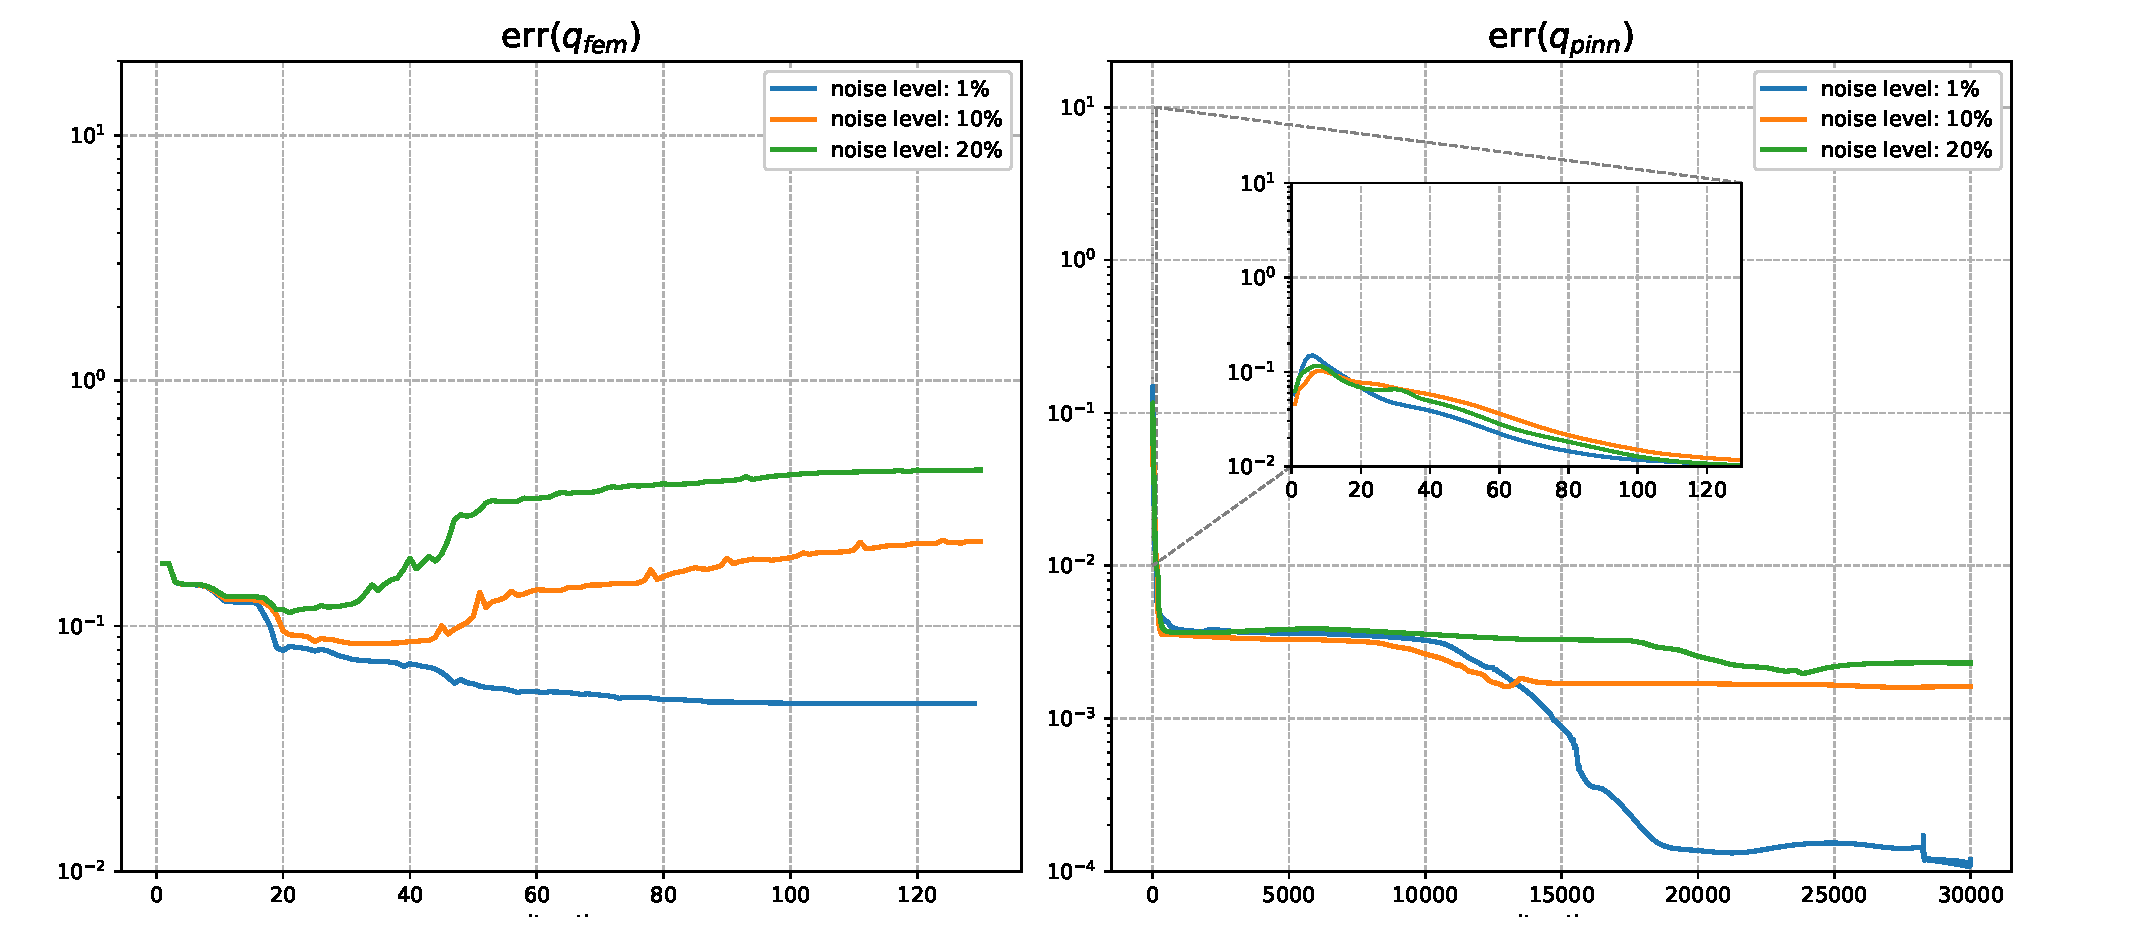
\includegraphics[width=\textwidth]{figures3/err_q.eps}
%    \caption{算例~\ref{example:nonsmooth} 中重构势函数 $q$ 的相对 $L^{2}$ 误差随迭代次数变化的曲线。左列显示了有限元方法获得的结果，而右列显示了 Tikhonov-PINNs 获得的结果。}
%    \label{fig:err_q}
% \end{figure}





\section{理论结果的证明}\label{sec:proof}
\subsection{稳定性的证明}\label{sec:lemma4}
在本小节中，我们将证明定理~\ref{th:potential:stability}，重述如下：

\begin{theorem}[稳定性估计]
在 Eq.\eqref{eq:pde:potential} 和 \eqref{eq:measurement} 的模型下。令 $(q^{\dagger},u^{\dagger})$ 满足 Eq.\eqref{eq:pde:potential}。假设假设 \ref{ass:potential:qudaggerreg} 成立，那么对于每一对满足 $q\in H^{2}(\Omega)$ 的 $(q,u)$，有
\begin{equation*}
\|(q-q^{\dagger})u^{\dagger}\|_{L^{2}(\Omega)}\leq C(1+\lambda^{-1/4}\calL_{\lambda}^{1/4}(q,u))(\calL_{\lambda}^{1/4}(q,u)+\delta^{1/2}),
\end{equation*}
其中 $C$ 是一个依赖于 $d$, $\Omega$, $\alpha$, $\overline{q}$, $\|q^{\dagger}\|_{W^{2,\infty}(\Omega)}$ 和 $\|u^{\dagger}\|_{W^{2,\infty}(\Omega)}$ 的正常数。
\end{theorem}

\begin{proof}
对于每个函数 $\psi\in H^{2}(\Omega)$，有
\begin{align*}
&((q^{\dagger}-q)u^{\dagger},\psi)_{L^{2}(\Omega)} \\
&=(-\nabla\cdot(\alpha\nabla u^{\dagger})_{L^{2}(\Omega)}+q^{\dagger}u^{\dagger},\psi)_{L^{2}(\Omega)}-(-\nabla\cdot(\alpha\nabla u^{\dagger})+qu^{\dagger},\psi)_{L^{2}(\Omega)} \\
&=(f+\nabla\cdot(\alpha\nabla u)-qu,\psi)_{L^{2}(\Omega)}-(q(u^{\dagger}-u),\psi)_{L^{2}(\Omega)}+(\nabla\cdot(\alpha\nabla(u^{\dagger}-u)),\psi)_{L^{2}(\Omega)} \\
&=(f+\nabla\cdot(\alpha\nabla u)-qu,\psi)_{L^{2}(\Omega)}-(q(u^{\dagger}-u),\psi)_{L^{2}(\Omega)}+(u^{\dagger}-u,\nabla\cdot(\alpha\nabla\psi))_{L^{2}(\Omega)} \\
&\quad-(T(u-u^{\dagger}),\alpha\partial_{\nu}\psi)_{L^{2}(\partial\Omega)}+(\alpha\partial_{\nu}u-g,T\psi)_{L^{2}(\partial\Omega)},
\end{align*}
这里我们使用了格林公式以及 $(q^{\dagger},u^{\dagger})$ 满足 Eq.\eqref{eq:pde:potential} 这一事实。应用柯西-施瓦茨不等式和迹定理 \cite[Theorem 1 in Section 5.5]{evans2010partial}，我们有
\begin{align*}
&((q-q^{\dagger})u^{\dagger},\psi)_{L^{2}(\Omega)} \\
&\leq C\big\{\|f+\nabla\cdot(\alpha\nabla u)-qu\|_{L^{2}(\Omega)}+\|q\|_{L^{\infty}(\Omega)}\|u-u^{\dagger}\|_{L^{2}(\Omega)}+\|u-u^{\dagger}\|_{L^{2}(\Omega)} \\
&\quad+\|T(u-u^{\dagger})\|_{L^{2}(\partial\Omega)}+\|\alpha\partial_{\nu}u-g\|_{L^{2}(\partial\Omega)}\big\}(\|\alpha\|_{C^{1}(\bar\Omega)}\vee1)\|\psi\|_{H^{2}(\Omega)} \\
&\leq C\big\{\|f+\nabla\cdot(\alpha\nabla u)-qu\|_{L^{2}(\Omega)}+\|\alpha\partial_{\nu}u-g\|_{L^{2}(\partial\Omega)}+\|q\|_{L^{\infty}(\Omega)}\|z^{\delta}-u\|_{L^{2}(\Omega)} \\
&\quad+\|Tz^{\delta}-Tu\|_{L^{2}(\partial\Omega)}+(\|q\|_{L^{\infty}(\Omega)}+1)\delta\big\}(\|\alpha\|_{C^{1}(\bar\Omega)}\vee1)\|\psi\|_{H^{2}(\Omega)},
\end{align*}
其中最后一个不等式是由于 Eq.\eqref{eq:measurement}，且 $C$ 是一个仅依赖于 $\Omega$ 的常数。因此，由算术-几何均值不等式（AM-GM inequality）可得
\begin{equation*}
\|(q-q^{\dagger})u^{\dagger}\|_{(H^{2}(\Omega))^{*}}\leq 2C(\|q\|_{L^{\infty}(\Omega)}+1)(\|\alpha\|_{C^{1}(\bar\Omega)}\vee1)\Big\{\calL_{\lambda}^{1/2}(q,u)+\delta\Big\}.
\end{equation*}
最后，利用假设 \ref{ass:potential:qudaggerreg} 可得
\begin{align*}
\|(q-q^{\dagger})u^{\dagger}\|_{L^{2}(\Omega)}&\leq\|(q-q^{\dagger})u^{\dagger}\|_{H^{2}(\Omega)}^{1/2}\|(q-q^{\dagger})u^{\dagger}\|_{(H^{2}(\Omega))^{*}}^{1/2} \\
&\lesssim\|q^{\dagger}\|_{W^{2,\infty}(\Omega)}^{1/2}\|u^{\dagger}\|_{W^{2,\infty}(\Omega)}^{1/2}(1+\|q\|_{H^{2}(\Omega)}^{1/2})\|(q-q^{\dagger})u^{\dagger}\|_{(H^{2}(\Omega))^{*}}^{1/2} \\
&\leq C(1+\lambda^{-1/4}\calL_{\lambda}^{1/4}(q,u))(\calL_{\lambda}^{1/4}(q,u)+\delta^{1/2}),
\end{align*}
证明完毕。
\end{proof}


% \subsection{误差分解}\label{sec:lemma5}
% 本小节致力于建立超额风险（excess risk）的误差分解，将其分离为逼近项和泛化项。这一框架使得我们能够利用函数逼近理论和覆盖数估计来分别界定每一部分。首先，我们给出覆盖数和度量熵的定义如下。

% \begin{definition}[覆盖数与度量熵]
% \label{def:covering}
% 令 \(({\cal X},\|\cdot\|_{{\cal X}})\) 为一个度量空间，且 \({\cal Y}\subseteq{\cal X}\)。令 \(\tau>0\)。若对于任意 \(g\in{\calY}\)，都存在 \(g_{\tau}\in{\calY}_{\tau}\) 使得 \(\|g-g_{\tau}\|_{{\cal X}}\leq\tau\)，则我们称 \({\calY}_{\tau}\) 为 \({\calY}\) 的一个 \(\|\cdot\|_{{\cal X}}\) \(\tau\)-覆盖。此外，
% \begin{equation*}
%   N(\tau,{\calY},{\calX})=\min\left\{|{\calY}_{\tau}|\colon{\calY}_{\tau}\mbox{ 是 }{\calY}\mbox{ 的一个 }\|\cdot\|_{{\cal X}}\;\tau\mbox{-覆盖}\right\}
% \end{equation*}
% 被称为 \({\calY}\) 的 \(\|\cdot\|_{{\cal X}}\) \(\tau\)-覆盖数，而
% \begin{equation*}
%   H(\tau,{\calY},{\cal X})=\log N(\tau,{\calY},{\cal X})
% \end{equation*}
% 被称为 \({\calY}\) 的 \(\|\cdot\|_{{\cal X}}\) \(\tau\)-度量熵。
% \end{definition}

% \begin{lemma}\label{lemma:errdec}
%    假设 $\|q\|_{W^{2,\infty}(\Omega)},\|q^{\dagger}\|_{W^{2,\infty}(\Omega)}\leq B_{\calQ}$ 且 $\|u\|_{W^{2,\infty}(\Omega)},\|u^{\dagger}\|_{W^{2,\infty}(\Omega)}\leq B_{\calU}$。设 Assumption \ref{allcondition} 中的假设 (ii) 成立。令 $\euS=\{\euD_{\calI},\euD_{\calB},\euX_{\calI},\euX_{\calB}\}$。令 $(\hat{q},\hat{u})\in\calQ\times\calU$ 为由 \eqref{eq:erm} 定义的经验风险最小化子，则有
%    \begin{align*}
%    \bbE_{\euS}\big[\calE_{\lambda}(\hat{q},\hat{u})\big]
%    &\lesssim\inf_{\tau>0}\Big\{\Delta_{\calQ}H(\tau,\calQ,W^{2,\infty}(\Omega))+\Delta_{\calU}H(\tau,\calU,W^{2,\infty}(\Omega))+\Delta\tau\Big\} \\
%    &\quad+\inf_{(q,u)\in\calQ\times\calU}\calE_{\lambda}(q,u),
%    \end{align*}
%    其中 $\bbE_{\euS}$ 表示关于随机样本集 $\mathcal{S}$ 取的期望，且
%    \begin{align*}
%    \Delta_{\calQ}&=\Big\{\lambda B_{\calQ}^{2}\frac{|\Omega|}{n_{\calI}}+(B_{\alpha}^{2}B_{\calU}^{2}+B_{\calQ}^{2}B_{\calU}^{2}+B_{f}^{2})\frac{|\Omega|}{n_{\calI}}\Big\}, \\
%    \Delta_{\calU}&=\Big\{(B_{\calU}^{2}+\delta^{2})\Big(\frac{|\Omega|}{m_{\calI}}+\frac{|\partial\Omega|}{m_{\calB}}\Big)+(B_{\alpha}^{2}B_{\calU}^{2}+B_{\calQ}^{2}B_{\calU}^{2}+B_{f}^{2})\frac{|\Omega|}{n_{\calI}}+(B_{\alpha}^{2}B_{\calU}^{2}+B_{g}^{2})\frac{|\partial\Omega|}{n_{\calB}}\Big\}, \\
%    \Delta&=(|\Omega|+|\partial\Omega|)C(B_{\alpha},B_{f},B_{g})\{B_{\calQ}B_{\calU}(B_{\calQ}+B_{\calU})+\delta\}.
%    \end{align*}
% \end{lemma}

% \begin{proof}
% \par 首先，我们分别引入 $\calQ\subseteq W^{2,\infty}(\Omega)$ 和 $\calU\subseteq W^{2,\infty}(\Omega)$ 的 $W^{2,\infty}(\Omega)$ $\tau$-覆盖。令 $\tau>0$，并令 $\calQ_{\tau}$ 为 $\calQ$ 的 $W^{2,\infty}(\Omega)$ $\tau$-覆盖，$\calU_{\tau}$ 为 $\calU$ 的 $W^{2,\infty}(\Omega)$ $\tau$-覆盖，满足
% \begin{equation*}
% |\calU_{\tau}|=N(\tau,\calU,W^{2,\infty}(\Omega))\quad\text{and}\quad|\calQ_{\tau}|=N(\tau,\calQ,W^{2,\infty}(\Omega)).
% \end{equation*}
% 那么对于每个 $u\in\calU$ 和 $q\in\calQ$，存在 $u_{\tau}\in\calU_{\tau}$ 和 $q_{\tau}\in\calQ_{\tau}$ 使得 $\|u-u_{\tau}\|_{W^{2,\infty}(\Omega)}\leq\tau$ 且 $\|q-q_{\tau}\|_{W^{2,\infty}(\Omega)}\leq\tau$。不失一般性，我们假设 $\|q_{\tau}\|_{W^{2,\infty}(\Omega)}\leq B_{\calQ}$ 且 $\|u_{\tau}\|_{W^{2,\infty}(\Omega)}\leq B_{\calU}$。
% \par 由于 $(\hat{q},\hat{u})\in\calQ\times\calU$，对于每个 $\gamma>0$，以下不等式成立
% \begin{equation}\label{eq:proof:errordec:2}
% \bbE_{\euS}\big[\calE_{\lambda}(\hat{q},\hat{u})\big]\leq\bbE_{\euS}\Big[\sup_{(q,u)\in\calQ\times\calU}\calE_{\lambda}(q,u)-(1+\gamma)\what{\calE}_{\lambda}(q,u)\Big]+(1+\gamma)\bbE_{\euS}\big[\what{\calE}_{\lambda}(\hat{q},\hat{u})\big].
% \end{equation}
% 在接下来的证明中，我们要分别估计 Eq.\eqref{eq:proof:errordec:2} 右侧的两项。
% \par\noindent\emph{步骤 1. 估计 Eq.\eqref{eq:proof:errordec:2} 右侧的第一项。}
% \par 由上确界的凸性，Eq.\eqref{eq:proof:errordec:2} 中的第一项可以如下有界
% \begin{align*}
% &\bbE_{\euS}\Big[\sup_{(q,u)\in\calQ\times\calU}\calE_{\lambda}(q,u)-(1+\gamma)\what{\calE_{\lambda}}(q,u)\Big] \\
% &\leq\bbE_{\euD_{\calI}}\Big[\sup_{u\in\calU}\|u-u^{\dagger}\|_{L^{2}(\Omega)}^{2}-(1+\gamma)\|u-u^{\dagger}\|_{L^{2}(\euD_{\calI})}^{2}\Big] \\
% &\quad+\bbE_{\euD_{\calB}}\Big[\sup_{u\in\calU}\|Tu-Tu^{\dagger}\|_{L^{2}(\partial\Omega)}^{2}-(1+\gamma)\|Tu-Tu^{\dagger}\|_{L^{2}(\euD_{\calB})}^{2}\Big] \\
% &\quad+\bbE_{\euX_{\calI}}\Big[\sup_{(q,u)\in\calQ\times\calU}\calI(q,u)-(1+\gamma)\what{\calI}(q,u)\Big]+\bbE_{\euX_{\calB}}\Big[\sup_{u\in\calU}\calB(u)-(1+\gamma)\what{\calB}(u)\Big] \\
% &\quad+\lambda\bbE_{\euX_{\calI}}\Big[\sup_{q\in\calQ}\|q\|_{H^{2}(\Omega)}^{2}-(1+\gamma)\|q\|_{H^{2}(\euX_{\calI})}^{2}\Big].
% \end{align*}
% \par 为方便符号表示，我们定义 $\ell_{\calI}(x;u)=(u(x)-u^{\dagger}(x))^{2}$。那么显然有
% \begin{equation*}
% \|u-u^{\dagger}\|_{L^{2}(\Omega)}^{2}=\bbE_{x}\big[\ell_{\calI}(x;u)\big]\quad\text{and}\quad\|u-u^{\dagger}\|_{L^{2}(\euD_{\calI})}^{2}=\frac{|\Omega|}{m_{\calI}}\sum_{i=1}^{m_{\calI}}\ell_{\calI}(x_{i}^{\calI};u).
% \end{equation*}
% 由于 $\|u\|_{W^{2,\infty}(\Omega)}\leq B_{\calU}$，我们发现对于每个 $x\in\Omega$，有 $0\leq\ell_{\calI}(x;u)\leq4B_{\calU}^{2}$ 且 $\ell_{\calI}^{2}(x;u)\leq4B_{\calU}^{2}\ell_{\calI}(x;u)$。那么通过一些代数运算可得
% \begin{align}
% &\bbE_{\euD_{\calI}}\Big[\sup_{u\in\calU}\|u-u^{\dagger}\|_{L^{2}(\Omega)}^{2}-(1+\gamma)\|u-u^{\dagger}\|_{L^{2}(\euD_{\calI})}^{2}\Big] \nonumber \\
% &=\bbE_{\euD_{\calI}}\Big[\sup_{u\in\calU}\frac{\gamma+2}{2}\bbE_{x}\big[\ell_{\calI}(x;u)\big]-\frac{\gamma}{2}\bbE_{x}\big[\ell_{\calI}(x;u)\big] \nonumber \\
% &\quad\quad\quad\quad-\frac{\gamma+2}{2}\frac{|\Omega|}{m_{\calI}}\sum_{i=1}^{m_{\calI}}\ell_{\calI}(x_{i}^{\calI};u)-\frac{\gamma}{2}\frac{|\Omega|}{m_{\calI}}\sum_{i=1}^{m_{\calI}}\ell_{\calI}(x_{i}^{\calI};u)\Big] \nonumber \\
% &\leq\bbE_{\euD_{\calI}}\Big[\sup_{u\in\calU}\frac{\gamma+2}{2}\bbE_{x}\big[\ell_{\calI}(x;u)\big]-\frac{\gamma}{8B_{\calU}^{2}}\bbE_{x}\big[\ell_{\calI}^{2}(x;u)\big] \nonumber \\
% &\quad\quad\quad\quad-\frac{\gamma+2}{2}\frac{|\Omega|}{m_{\calI}}\sum_{i=1}^{m_{\calI}}\ell_{\calI}(x_{i}^{\calI};u)-\frac{\gamma}{8B_{\calU}^{2}}\frac{|\Omega|}{m_{\calI}}\sum_{i=1}^{m_{\calI}}\ell_{\calI}^{2}(x_{i}^{\calI};u)\Big]. \label{eq:proof:errordec:3}
% \end{align}
% 令 $\tilde{\euD}_{\calI}=\{(\tilde{x}_{i},\tilde{z}_{i}^{\delta})\}_{i=1}^{m_{\calI}}$ 为一个幽灵样本（ghost sample），这意味着 $\{(\tilde{x}_{i},\tilde{z}_{i}^{\delta})\}_{i=1}^{m_{\calI}}$ 是独立地从 Eq.\eqref{eq:measurement} 中抽取，且独立于 $\euD_{\calI}$。假设 $\xi=\{\xi_{i}\}_{i=1}^{m_{\calI}}$ 是一系列独立同分布的 Rademacher 变量，且独立于 $\euD_{\calI}$ 和 $\tilde{\euD}_{\calI}$。那么，利用对称化（symmetrization）技术，可得
% \begin{align}
% &\bbE_{\euD_{\calI}}\Big[\sup_{u\in\calU}\frac{\gamma+2}{2}\bbE_{x}\big[\ell_{\calI}(x;u)\big]-\frac{\gamma}{8B_{\calU}^{2}}\bbE_{x}\big[\ell_{\calI}^{2}(x;u)\big] \nonumber \\
% &\quad\quad\quad\quad-\frac{\gamma+2}{2}\frac{|\Omega|}{m_{\calI}}\sum_{i=1}^{m_{\calI}}\ell_{\calI}(x_{i}^{\calI};u)-\frac{\gamma}{8B_{\calU}^{2}}\frac{|\Omega|}{m_{\calI}}\sum_{i=1}^{m_{\calI}}\ell_{\calI}^{2}(x_{i}^{\calI};u)\Big] \nonumber \\
% &\leq\bbE_{\euD_{\calI}}\Big[\sup_{u\in\calU}\bbE_{\tilde{\euD}_{\calI}}\Big[\frac{\gamma+2}{2}\frac{|\Omega|}{m_{\calI}}\sum_{i=1}^{m_{\calI}}\ell_{\calI}(\tilde{x}_{i}^{\calI};u)-\frac{\gamma}{8B_{\calU}^{2}}\frac{|\Omega|}{m_{\calI}}\sum_{i=1}^{m_{\calI}}\ell_{\calI}^{2}(\tilde{x}_{i}^{\calI};u)\Big] \nonumber \\
% &\quad\quad\quad\quad-\frac{\gamma+2}{2}\frac{|\Omega|}{m_{\calI}}\sum_{i=1}^{m_{\calI}}\ell_{\calI}(x_{i}^{\calI};u)-\frac{\gamma}{8B_{\calU}^{2}}\frac{|\Omega|}{m_{\calI}}\sum_{i=1}^{m_{\calI}}\ell_{\calI}^{2}(x_{i}^{\calI};u)\Big] \nonumber \\
% &\leq\bbE_{\euD_{\calI}}\bbE_{\tilde{\euD}_{\calI}}\Big[\sup_{u\in\calU}\frac{\gamma+2}{2}\frac{|\Omega|}{m_{\calI}}\sum_{i=1}^{m_{\calI}}(\ell_{\calI}(\tilde{x}_{i}^{\calI};u)-\ell_{\calI}(x_{i}^{\calI};u)) \nonumber \\
% &\quad\quad\quad\quad-\frac{\gamma}{8B_{\calU}^{2}}\frac{|\Omega|}{m_{\calI}}\sum_{i=1}^{m_{\calI}}(\ell_{\calI}^{2}(\tilde{x}_{i}^{\calI};u)+\ell_{\calI}^{2}(x_{i}^{\calI};u))\Big] \nonumber \\
% &=\bbE_{\euD_{\calI}}\bbE_{\tilde{\euD}_{\calI}}\bbE_{\xi}\Big[\sup_{u\in\calU}\frac{\gamma+2}{2}\frac{|\Omega|}{m_{\calI}}\sum_{i=1}^{m_{\calI}}\xi_{i}(\ell_{\calI}(\tilde{x}_{i}^{\calI};u)-\ell_{\calI}(x_{i}^{\calI};u)) \nonumber \\
% &\quad\quad\quad\quad-\frac{\gamma}{8B_{\calU}^{2}}\frac{|\Omega|}{m_{\calI}}\sum_{i=1}^{m_{\calI}}(\ell_{\calI}^{2}(\tilde{x}_{i}^{\calI};u)+\ell_{\calI}^{2}(x_{i}^{\calI};u))\Big] \nonumber \\
% &=\bbE_{\euD_{\calI}}\bbE_{\xi}\Big[\sup_{u\in\calU}(\gamma+2)\frac{|\Omega|}{m_{\calI}}\sum_{i=1}^{m_{\calI}}\xi_{i}\ell_{\calI}(x_{i}^{\calI};u)-\frac{\gamma}{4B_{\calU}^{2}}\frac{|\Omega|}{m_{\calI}}\sum_{i=1}^{m_{\calI}}\ell_{\calI}^{2}(x_{i}^{\calI};u)\Big], \label{eq:proof:errordec:4}
% \end{align}
% 其中第二个不等式由 Jensen 不等式成立，且 $\bbE_{\xi}[\cdot]=\bbE[\cdot|\euD_{\calI},\tilde{\euD}_{\calI}]$ 表示关于 $\euD_{\calI}$ 和 $\tilde{\euD}_{\calI}$ 的条件期望。
% \par 我们现在转向估计最后一行的条件期望。回顾 $\calU_{\tau}$ 的定义，对于每个 $u\in\calU$，存在 $u_{\tau}\in\calU_{\tau}$ 使得 $\|u-u_{\tau}\|_{W^{2,\infty}(\Omega)}\leq\tau$，并注意到
% \begin{equation*}
% |\ell_{\calI}(x_{i}^{\calI};u)-\ell_{\calI}(x_{i}^{\calI};u_{\tau})|\leq 4B_{\calU}\tau.
% \end{equation*}
% 因此，我们发现
% \begin{align*}
% &(\gamma+2)\frac{|\Omega|}{m_{\calI}}\sum_{i=1}^{m_{\calI}}\xi_{i}\ell_{\calI}(x_{i}^{\calI};u) \\
% &\leq(\gamma+2)\frac{|\Omega|}{m_{\calI}}\sum_{i=1}^{m_{\calI}}\xi_{i}\ell_{\calI}(x_{i}^{\calI};u_{\tau})+(\gamma+2)\frac{|\Omega|}{m_{\calI}}\sum_{i=1}^{m_{\calI}}|\ell_{\calI}(x_{i}^{\calI};u)-\ell_{\calI}(x_{i}^{\calI};u_{\tau})| \\
% &\leq(\gamma+2)\frac{|\Omega|}{m_{\calI}}\sum_{i=1}^{m_{\calI}}\xi_{i}\ell_{\calI}(x_{i}^{\calI};u_{\tau})+4(\gamma+2)|\Omega|B_{\calU}\tau,
% \end{align*}
% 以及
% \begin{align*}
% &-\frac{\gamma}{4B_{\calU}^{2}}\frac{|\Omega|}{m_{\calI}}\sum_{i=1}^{m_{\calI}}\ell_{\calI}^{2}(x_{i}^{\calI};u) \\
% &\leq-\frac{\gamma}{4B_{\calU}^{2}}\frac{|\Omega|}{m_{\calI}}\sum_{i=1}^{m_{\calI}}\ell_{\calI}^{2}(x_{i}^{\calI};u_{\tau})+2\gamma\frac{|\Omega|}{m_{\calI}}\sum_{i=1}^{m_{\calI}}|\ell_{\calI}(x_{i}^{\calI};u_{\tau})-\ell_{\calI}(x_{i}^{\calI};u)| \\
% &\leq-\frac{\gamma}{4B_{\calU}^{2}}\frac{|\Omega|}{m_{\calI}}\sum_{i=1}^{m_{\calI}}\ell_{\calI}^{2}(x_{i}^{\calI};u_{\tau})+8\gamma|\Omega|B_{\calU}\tau.
% \end{align*}
% 从而
% \begin{equation}\label{eq:proof:errordec:5}
% \begin{aligned}
% &\bbE\Big[\sup_{u\in\calU}(\gamma+2)\frac{|\Omega|}{m_{\calI}}\sum_{i=1}^{m_{\calI}}\xi_{i}\ell_{\calI}(x_{i}^{\calI};u)-\frac{\gamma}{4B_{\calU}^{2}}\frac{|\Omega|}{m_{\calI}}\sum_{i=1}^{m_{\calI}}\ell_{\calI}^{2}(x_{i}^{\calI};u)\Big|\euD_{\calI}\Big] \\
% &\leq\bbE\Big[\sup_{u_{\tau}\in\calU_{\tau}}(\gamma+2)\frac{|\Omega|}{m_{\calI}}\sum_{i=1}^{m_{\calI}}\xi_{i}\ell_{\calI}(x_{i}^{\calI};u_{\tau})-\frac{\gamma}{4B_{\calU}^{2}}\frac{|\Omega|}{m_{\calI}}\sum_{i=1}^{m_{\calI}}\ell_{\calI}^{2}(x_{i}^{\calI};u_{\tau})\Big|\euD_{\calI}\Big] \\
% &\quad+4(3\gamma+2)|\Omega|B_{\calU}\tau.
% \end{aligned}
% \end{equation}
% 由于 $\{\xi_{i}\ell_{\calI}(x_{i}^{\calI};u_{\tau})\}_{i=1}^{m_{\calI}}$ 是以 $\euD_{\calI}$ 为条件的独立随机变量，因此 $\bbE[\xi_{i}\ell_{\calI}(x_{i}^{\calI};u_{\tau})\big|\euD_{\calI}]=0$ 且 $-\ell_{\calI}(x_{i}^{\calI};u_{\tau})\leq\xi_{i}\ell_{\calI}(x_{i}^{\calI};u_{\tau})\leq\ell_{\calI}(x_{i}^{\calI};u_{\tau})$。接着使用 Hoeffding 不等式 \cite[Theorem D.2]{mohri2018foundations} 可得
% \begin{align*}
% &\bbP\Big\{(\gamma+2)\frac{|\Omega|}{m_{\calI}}\sum_{i=1}^{m_{\calI}}\xi_{i}\ell_{\calI}(x_{i}^{\calI};u_{\tau})>t+\frac{\gamma}{4B_{\calU}^{2}}\frac{|\Omega|}{m_{\calI}}\sum_{i=1}^{m_{\calI}}\ell_{\calI}^{2}(x_{i}^{\calI};u_{\tau})\Big|\euD_{\calI}\Big\} \\
% &=\bbP\Big\{\sum_{i=1}^{m_{\calI}}\xi_{i}\ell_{\calI}(x_{i}^{\calI};u_{\tau})>\frac{1}{\gamma+2}\frac{m_{\calI}}{|\Omega|}t+\frac{\gamma}{\gamma+2}\frac{1}{4B_{\calU}^{2}}\sum_{i=1}^{m_{\calI}}\ell_{\calI}^{2}(x_{i}^{\calI};u_{\tau})\Big|\euD_{\calI}\Big\} \\
% &\leq\exp\Big(-\frac{(\frac{\gamma}{\gamma+2}\frac{1}{4B_{\calU}^{2}})^{2}}{2}\frac{(\frac{4B_{\calU}^{2}}{\gamma}\frac{m_{\calI}}{|\Omega|}t+\sum_{i=1}^{m_{\calI}}\ell_{\calI}^{2}(x_{i}^{\calI};u_{\tau}))^{2}}{\sum_{i=1}^{m_{\calI}}\ell_{\calI}^{2}(x_{i}^{\calI};u_{\tau})}\Big) \\
% &\leq\exp\Big(-\frac{\gamma}{(\gamma+2)^{2}}\frac{1}{2B_{\calU}^{2}}\frac{m_{\calI}}{|\Omega|}t\Big),
% \end{align*}
% 其中最后一个不等式源自数值不等式
% \begin{equation*}
% \frac{(a+y)^{2}}{y}\geq\frac{(a+a)^{2}}{a}=4a,\quad y\in\bbR_{+}.
% \end{equation*}
% 对于任意 $T>0$，有
% \begin{align*}
% &\bbE\Big[\sup_{u_{\tau}\in\calU_{\tau}}(\gamma+2)\frac{|\Omega|}{m_{\calI}}\sum_{i=1}^{m_{\calI}}\xi_{i}\ell_{\calI}(x_{i}^{\calI};u_{\tau})-\frac{\gamma}{4B_{\calU}^{2}}\frac{|\Omega|}{m_{\calI}}\sum_{i=1}^{m_{\calI}}\ell_{\calI}^{2}(x_{i}^{\calI};u_{\tau})\Big|\euD_{\calI}\Big] \\
% &=\int_{0}^{\infty}\bbP\Big\{\sup_{u_{\tau}\in\calU_{\tau}}(\gamma+2)\frac{|\Omega|}{m_{\calI}}\sum_{i=1}^{m_{\calI}}\xi_{i}\ell_{\calI}(x_{i}^{\calI};u_{\tau})-\frac{\gamma}{4B_{\calU}^{2}}\frac{|\Omega|}{m_{\calI}}\sum_{i=1}^{m_{\calI}}\ell_{\calI}^{2}(x_{i}^{\calI};u_{\tau})>t\Big|\euD_{\calI}\Big\}dt \\
% &\leq T+\frac{(\gamma+2)^{2}}{\gamma}2B_{\calU}^{2}\frac{|\Omega|}{m_{\calI}}|\calU_{\tau}|\exp\Big(-\frac{\gamma}{(\gamma+2)^{2}}\frac{1}{2B_{\calU}^{2}}\frac{m_{\calI}}{|\Omega|}T\Big).
% \end{align*}
% 将
% $$T=\frac{(\gamma+2)^{2}}{\gamma}2B_{\calU}^{2}\frac{|\Omega|}{m_{\calI}}\log|\calU_{\tau}|$$
% 代入上述不等式，并结合 Eq.\eqref{eq:proof:errordec:3}、Eq.\eqref{eq:proof:errordec:4} 和 Eq.\eqref{eq:proof:errordec:5}，我们得到
% \begin{align}
% &\bbE_{\euD_{\calI}}\bbE_{\xi}\Big[\sup_{u\in\calU}(\gamma+2)\frac{|\Omega|}{m_{\calI}}\sum_{i=1}^{m_{\calI}}\xi_{i}\ell_{\calI}(x_{i}^{\calI};u)-\frac{\gamma}{4B_{\calU}^{2}}\frac{|\Omega|}{m_{\calI}}\sum_{i=1}^{m_{\calI}}\ell_{\calI}^{2}(x_{i}^{\calI};u)\Big] \nonumber \\
% &\leq2(\gamma+2)^{2}\gamma^{-1}|\Omega|B_{\calU}^{2}m_{\calI}^{-1}(1+\log|\calU_{\tau}|)+2(3\gamma+2)|\Omega|B_{\calU}\tau.\label{eq:proof:errordec:6}
% \end{align}


% 类似地，我们定义 $\ell_{\calB}(x;u)=(Tu(x)-Tu^{\dagger}(x))^{2}$，且下列不等式成立
% \begin{align}
% &\bbE_{\euD_{\calB}}\Big[\sup_{u\in\calU}\|Tu-Tu^{\dagger}\|_{L^{2}(\partial\Omega)}^{2}-(1+\gamma)\|Tu-Tu^{\dagger}\|_{L^{2}(\euD_{\calB})}^{2}\Big] \nonumber \\
% &\leq\bbE_{\euD_{\calB}}\bbE_{\xi}\Big[\sup_{u\in\calU}(\gamma+2)\frac{|\partial\Omega|}{m_{\calB}}\sum_{i=1}^{m_{\calB}}\xi_{i}\ell_{\calB}(x_{i}^{\calB};u)-\frac{\gamma}{4B_{\calU}^{2}}\frac{|\partial\Omega|}{m_{\calB}}\sum_{i=1}^{m_{\calB}}\ell_{\calB}^{2}(x_{i}^{\calB};u)\Big] \nonumber \\
% &\leq2(\gamma+2)^{2}\gamma^{-1}|\partial\Omega|B_{\calU}^{2}m_{\calB}^{-1}(1+\log|\calU_{\tau}|)+2(3\gamma+2)|\partial\Omega|B_{\calU}\tau.\label{eq:proof:errordec:7}
% \end{align}
% \par 定义 $p_{\calI}(x;q,u)=(\nabla\cdot(\alpha(x)\nabla u(x))-q(x)u(x)+f(x))^{2}$，并注意到
% \begin{align*}
% &0\leq p_{\calI}(x_{j}^{\calI};q,u)\leq4B_{\alpha}^{2}B_{\calU}^{2}+4B_{\calQ}^{2}B_{\calU}^{2}+4B_{f}^{2}=:B_{p,\calI}^{2}, \\
% &|p_{\calI}(x_{j}^{\calI};q,u)-p_{\calI}(x_{j}^{\calI};q_{\tau},u_{\tau})| \\
% &\leq(2B_{\alpha}B_{\calU}+2B_{\calQ}B_{\calU}+2B_{f})(B_{\alpha}+B_{\calQ}+B_{\calU})\tau=:L_{p,\calI}\tau.
% \end{align*}
% 类似于 Eq.\eqref{eq:proof:errordec:3} 和 Eq.\eqref{eq:proof:errordec:4} 的证明，下列不等式成立
% \begin{align*}
% &\bbE_{\euX_{\calI}}\Big[\sup_{(q,u)\in\calQ\times\calU}\calI(q,u)-(1+\gamma)\what{\calI}(q,u)\Big] \\
% &\leq\bbE_{\euX_{\calI}}\bbE_{\xi}\Big[\sup_{(q,u)\in\calQ\times\calU}(\gamma+2)\frac{|\Omega|}{n_{\calI}}\sum_{j=1}^{n_{\calI}}\xi_{j}p_{\calI}(x_{j}^{\calI};q,u)-\frac{\gamma}{B_{p,\calI}^{2}}\frac{|\Omega|}{n_{\calI}}\sum_{j=1}^{n_{\calI}}p_{\calI}^{2}(x_{j}^{\calI};q,u)\Big],
% \end{align*}
% 其中 $\xi=\{\xi_{j}\}_{j=1}^{n_{\calI}}$ 是独立于 $\euX_{\calI}$ 的独立同分布 (i.i.d.) Rademacher 变量序列。回顾 $\tau$-覆盖 $\calQ_{\tau}$ 和 $\calU_{\tau}$，对于任意 $(q,u)\in\calQ\times\calU$，存在 $(q_{\tau},u_{\tau})\in\calQ_{\tau}\times\calU_{\tau}$ 使得
% \begin{align*}
% (\gamma+2)\frac{|\Omega|}{n_{\calI}}\sum_{j=1}^{n_{\calI}}\xi_{j}p_{\calI}(x_{j}^{\calI};q,u)&\leq(\gamma+2)\frac{|\Omega|}{n_{\calI}}\sum_{j=1}^{n_{\calI}}\xi_{j}p_{\calI}(x_{j}^{\calI};q_{\tau},u_{\tau})+(\gamma+2)|\Omega|L_{p,\calI}\tau, \\
% -\frac{\gamma}{B_{p,\calI}^{2}}\frac{|\Omega|}{n_{\calI}}\sum_{j=1}^{n_{\calI}}p_{\calI}^{2}(x_{j}^{\calI};q,u)&\leq-\frac{\gamma}{B_{p,\calI}^{2}}\frac{|\Omega|}{n_{\calI}}\sum_{j=1}^{n_{\calI}}p_{\calI}^{2}(x_{j}^{\calI};q_{\tau},u_{\tau})+2\gamma|\Omega|L_{p,\calI}\tau.
% \end{align*}
% 从而，
% \begin{align*}
% &\bbE\Big[\sup_{(q,u)\in\calQ\times\calU}(\gamma+2)\frac{|\Omega|}{n_{\calI}}\sum_{j=1}^{n_{\calI}}\xi_{j}p_{\calI}(x_{j}^{\calI};q,u)-\frac{\gamma}{B_{p,\calI}^{2}}\frac{|\Omega|}{n_{\calI}}\sum_{j=1}^{n_{\calI}}p_{\calI}^{2}(x_{j}^{\calI};q,u)\Big|\euX_{\calI}\Big] \\
% &\leq\bbE\Big[\sup_{(q_{\tau},u_{\tau})\in\calQ_{\tau}\times\calU_{\tau}}(\gamma+2)\frac{|\Omega|}{n_{\calI}}\sum_{j=1}^{n_{\calI}}\xi_{j}p_{\calI}(x_{j}^{\calI};q_{\tau},u_{\tau})-\frac{\gamma}{B_{p,\calI}^{2}}\frac{|\Omega|}{n_{\calI}}\sum_{j=1}^{n_{\calI}}p_{\calI}^{2}(x_{j}^{\calI};q_{\tau},u_{\tau})\Big|\euX_{\calI}\Big] \\
% &\quad+(3\gamma+2)|\Omega|L_{p,\calI}\tau.
% \end{align*}
% 在估计条件期望之前，我们首先通过下列不等式对尾概率进行控制
% \begin{align*}
% &\bbP\Big\{(\gamma+2)\frac{|\Omega|}{n_{\calI}}\sum_{j=1}^{n_{\calI}}\xi_{j}p_{\calI}(x_{j}^{\calI};q_{\tau},u_{\tau})>t+\frac{\gamma}{B_{p,\calI}^{2}}\frac{|\Omega|}{n_{\calI}}\sum_{j=1}^{n_{\calI}}p_{\calI}^{2}(x_{j}^{\calI};q_{\tau},u_{\tau})\Big|\euX_{\calI}\Big\} \\
% &\leq\exp\Big(-\frac{\gamma}{(\gamma+2)^{2}}\frac{2}{B_{p,\calI}^{2}}\frac{n_{\calI}}{|\Omega|}t\Big),
% \end{align*}
% 对于任意 $(q_{\tau},u_{\tau})\in\calQ_{\tau}\times\calU_{\tau}$，由此推导出
% \begin{align*}
% &\bbP\Big\{\sup_{(q_{\tau},u_{\tau})\in\calQ_{\tau}\times\calU_{\tau}}(\gamma+2)\frac{|\Omega|}{n_{\calI}}\sum_{j=1}^{n_{\calI}}\xi_{j}p_{\calI}(x_{j}^{\calI};q_{\tau},u_{\tau})-\frac{\gamma}{B_{p,\calI}^{2}}\frac{|\Omega|}{n_{\calI}}\sum_{j=1}^{n_{\calI}}p_{\calI}^{2}(x_{j}^{\calI};q_{\tau},u_{\tau})>t\Big|\euX_{\calI}\Big\} \\
% &\leq|\calQ_{\tau}||\calU_{\tau}|\exp\Big(-\frac{\gamma}{(\gamma+2)^{2}}\frac{2}{B_{p,\calI}^{2}}\frac{n_{\calI}}{|\Omega|}t\Big).
% \end{align*}
% 结合上述论证可得
% \begin{equation}\label{eq:proof:errordec:8}
% \begin{aligned}
% &\bbE_{\euX_{\calI}}\Big[\sup_{(q,u)\in\calQ\times\calU}\calI(q,u)-(1+\gamma)\what{\calI}(q,u)\Big] \\
% &\leq2(\gamma+2)^{2}\gamma^{-1}|\Omega|(B_{\alpha}^{2}B_{\calU}^{2}+B_{\calQ}^{2}B_{\calU}^{2}+B_{f}^{2})n_{\calI}^{-1}(1+\log|\calQ_{\tau}|+\log|\calU_{\tau}|) \\
% &\quad+2(3\gamma+2)|\Omega|(B_{\alpha}B_{\calU}+B_{\calQ}B_{\calU}+B_{f})(B_{\alpha}+B_{\calQ}+B_{\calU})\tau.
% \end{aligned}
% \end{equation}
% \par 同理，我们定义 $p_{\calB}(x;u)=(\alpha(x)\partial_{\nu}u(x)-g(x))^{2}$ 并发现
% \begin{align*}
% &0\leq p_{\calB}(x_{j}^{\calB};u)\leq2B_{\alpha}^{2}B_{\calU}^{2}+2B_{g}^{2}=:B_{p,\calB}, \\
% &|p_{\calB}(x_{j}^{\calB};u)-p_{\calB}(x_{j}^{\calB};\tilde{u})|\leq(B_{\alpha}B_{\calU}+B_{g})B_{\alpha}\tau.
% \end{align*}
% 因此，成立
% \begin{equation}\label{eq:proof:errordec:9}
% \begin{aligned}
% &\bbE_{\euX_{\calB}}\Big[\sup_{u\in\calU}\calB(u)-(1+\gamma)\what{\calB}(u)\Big]  \\
% &\leq\bbE_{\euX_{\calB}}\bbE_{\xi}\Big[\sup_{u\in\calU}\frac{\gamma+2}{2}\frac{|\partial\Omega|}{n_{\calB}}\sum_{j=1}^{n_{\calB}}\xi_{j}p_{\calB}(x_{j}^{\calB};u)-\frac{\gamma}{B_{p,\calB}^{2}}\frac{|\partial\Omega|}{n_{\calB}}\sum_{j=1}^{n_{\calB}}p_{\calB}^{2}(x_{j}^{\calB};u)\Big]  \\
% &\leq(\gamma+2)^{2}\gamma^{-1}|\partial\Omega|(B_{\alpha}^{2}B_{\calU}^{2}+B_{g}^{2})n_{\calB}^{-1}(1+\log|\calU_{\tau}|) \\
% &\quad+(3\gamma+2)|\partial\Omega|(B_{\alpha}B_{\calU}+B_{g})B_{\alpha}\tau.
% \end{aligned}
% \end{equation}
% 进一步，定义 $r(x;q)=q(x)^{2}+\sum_{k=1}^{d}\partial_{k}q(x)^{2}+\sum_{k=1}^{d}\sum_{\ell=1}^{d}\partial_{k}\partial_{\ell}q(x)^{2}$。据此可得
% \begin{equation}\label{eq:proof:errordec:10}
% \begin{aligned}
% &\bbE_{\euX_{\calI}}\Big[\sup_{q\in\calQ}\|q\|_{H^{2}(\Omega)}^{2}-(1+\gamma)\|q\|_{H^{2}(\euX_{\calI})}^{2}\Big] \\
% &\leq\bbE_{\euX_{\calI}}\bbE_{\xi}\Big[\sup_{q\in\calQ}(\gamma+2)\frac{|\Omega|}{n_{\calI}}\sum_{j=1}^{n_{\calI}}\xi_{j}r(x_{j}^{\calI};q)-\frac{\gamma}{B_{\calQ}^{2}}\frac{|\Omega|}{n_{\calI}}\sum_{j=1}^{n_{\calI}}r^{2}(x_{j}^{\calI};q)\Big] \\
% &\leq2^{-1}(\gamma+2)^{2}\gamma^{-1}|\Omega|B_{\calQ}^{2}n_{\calI}^{-1}(1+\log|\calQ_{\tau}|)+(3\gamma+2)|\Omega|B_{\calQ}\tau.
% \end{aligned}
% \end{equation}
% \par 最后，结合 Eq.\eqref{eq:proof:errordec:6} 至 Eq.\eqref{eq:proof:errordec:10} 可得
% \begin{align*}
% &\bbE_{\euS}\Big[\sup_{(q,u)\in\calQ\times\calU}\calE_{\lambda}(q,u)-(1+\gamma)\what{\calE}_{\lambda}(q,u)\Big] \\
% &\leq4\frac{(\gamma+2)^{2}}{\gamma}\Big\{\Delta_{\calQ}\log|\calQ_{\tau}|+\Delta_{\calU}\log|\calU_{\tau}|\Big\}+(3\gamma+2)\Delta\tau,
% \end{align*}
% 其中
% \begin{align*}
% \Delta_{\calQ}&=\Big\{\lambda B_{\calQ}^{2}\frac{|\Omega|}{n_{\calI}}+(B_{\alpha}^{2}B_{\calU}^{2}+B_{\calQ}^{2}B_{\calU}^{2}+B_{f}^{2})\frac{|\Omega|}{n_{\calI}}\Big\}, \\
% \Delta_{\calU}&=\Big\{B_{\calU}^{2}\Big(\frac{|\Omega|}{m_{\calI}}+\frac{|\partial\Omega|}{m_{\calB}}\Big)+(B_{\alpha}^{2}B_{\calU}^{2}+B_{\calQ}^{2}B_{\calU}^{2}+B_{f}^{2})\frac{|\Omega|}{n_{\calI}}+(B_{\alpha}^{2}B_{\calU}^{2}+B_{g}^{2})\frac{|\partial\Omega|}{n_{\calB}}\Big\}, \\
% \Delta&=(|\Omega|+|\partial\Omega|)C(B_{\alpha},B_{f},B_{g})B_{\calQ}B_{\calU}(B_{\calQ}+B_{\calU}).
% \end{align*}

% \par\noindent\emph{第 2 步。估计 Eq.\eqref{eq:proof:errordec:2} 右端的第二项。}
% 根据 Eq.\eqref{eq:measurement}，可得
% \begin{eqnarray*}
% % \nonumber % Remove numbering (before each equation)
%   \|\hat{u}-z^{\delta}\|_{L^{2}(\euD_{\calI})}^{2} &=& \|\hat{u}-u^{\dagger}\|_{L^{2}(\euD_{\calI})}^{2}-\frac{2|\Omega|}{m_{\calI}}\sum_{i=1}^{m_{\calI}}\varepsilon_{\calI}(x_{i}^{\calI})(\hat{u}(x_{i}^{\calI})-u^{\dagger}(x_{i}^{\calI})) \\
%    &+& \frac{|\Omega|}{m_{\calI}}\sum_{i=1}^{m_{\calI}}\varepsilon_{\calI}(x_{i}^{\calI})^{2},
% \end{eqnarray*}
% 这意味着对于每个 $u\in\calU$，
% \begin{align*}
% &\bbE_{\euD_{\calI}}\Big[\|\hat{u}-u^{\dagger}\|_{L^{2}(\euD_{\calI})}^{2}\Big] \\
% &=\bbE_{\euD_{\calI}}\Big[\|\hat{u}-z^{\delta}\|_{L^{2}(\euD_{\calI})}^{2}\Big]+2\bbE_{\euD_{\calI}}\Big[\frac{|\Omega|}{m_{\calI}}\sum_{i=1}^{m_{\calI}}\varepsilon_{\calI}(x_{i}^{\calI})\hat{u}(x_{i}^{\calI})\Big]-|\Omega|\delta^{2},
% \end{align*}
% 其中我们利用了 $\bbE[\sum_{i}\varepsilon_{\calI}(x_{i}^{\calI})u^{\dagger}(x_{i}^{\calI})]=0$ 这一事实。同理，我们发现
% \begin{align*}
% &\bbE_{\euD_{\calB}}\Big[\|T\hat{u}-Tu^{\dagger}\|_{L^{2}(\euD_{\calB})}^{2}\Big] \\
% &\leq\bbE_{\euD_{\calB}}\Big[\|T\hat{u}-Tz^{\delta}\|_{L^{2}(\euD_{\calB})}^{2}\Big]+2\bbE_{\euD_{\calB}}\Big[\frac{|\partial\Omega|}{m_{\calB}}\sum_{i=1}^{m_{\calB}}\varepsilon_{\calB}(x_{i}^{\calB})\hat{u}(x_{i}^{\calB})\Big]-|\partial\Omega|\delta^{2}.
% \end{align*}
% 从而，可得
% \begin{align*}
% \bbE_{\euS}\big[\what{\calE}(\hat{q},\hat{u})\big]&\leq\bbE_{\euD_{\calI},\euD_{\calB}}\Big[\|\hat{u}-z^{\delta}\|_{L^{2}(\euD_{\calI})}^{2}+\|T\hat{u}-Tz^{\delta}\|_{L^{2}(\euD_{\calB})}^{2}\Big]+\bbE_{\euX_{\calI},\euX_{\calB}}\Big[\what{\calI}(\hat{q},\hat{u})+\what{\calB}(\hat{u})\Big] \\
% &\quad+\lambda\bbE_{\euX_{\calI}}\Big[\|\hat{q}\|_{H^{2}(\euX_{\calI})}^{2}\Big]-\Big\{|\Omega|\delta^{2}+|\partial\Omega|\delta^{2}\Big\} \\
% &\quad+2\bbE_{\euD_{\calI}}\Big[\frac{|\Omega|}{m_{\calI}}\sum_{i=1}^{m_{\calI}}\varepsilon_{\calI}(x_{i}^{\calI})\hat{u}(x_{i}^{\calI})\Big]+2\bbE_{\euD_{\calB}}\Big[\frac{|\partial\Omega|}{m_{\calB}}\sum_{i=1}^{m_{\calB}}\varepsilon_{\calB}(x_{i}^{\calB})\hat{u}(x_{i}^{\calB})\Big] \\
% &=\bbE_{\euS}\Big[\what{\calL}_{\lambda}(\hat{q},\hat{u})\Big]-\calL(q^{\dagger},u^{\dagger})+2\bbE_{\euD_{\calI}}\Big[\frac{|\Omega|}{m_{\calI}}\sum_{i=1}^{m_{\calI}}\varepsilon_{\calI}(x_{i}^{\calI})\hat{u}(x_{i}^{\calI})\Big] \\
% &\quad+2\bbE_{\euD_{\calB}}\Big[\frac{|\partial\Omega|}{m_{\calB}}\sum_{i=1}^{m_{\calB}}\varepsilon_{\calB}(x_{i}^{\calB})\hat{u}(x_{i}^{\calB})\Big] \\
% &\leq\bbE_{\euS}\Big[\what{\calL}_{\lambda}(q,u)\Big]-\calL(q^{\dagger},u^{\dagger})+2\bbE_{\euD_{\calI}}\Big[\frac{|\Omega|}{m_{\calI}}\sum_{i=1}^{m_{\calI}}\varepsilon_{\calI}(x_{i}^{\calI})\hat{u}(x_{i}^{\calI})\Big] \\
% &\quad+2\bbE_{\euD_{\calB}}\Big[\frac{|\partial\Omega|}{m_{\calB}}\sum_{i=1}^{m_{\calB}}\varepsilon_{\calB}(x_{i}^{\calB})\hat{u}(x_{i}^{\calB})\Big] \\
% &=\calE_{\lambda}(q,u)+2\bbE_{\euD_{\calI}}\Big[\frac{|\Omega|}{m_{\calI}}\sum_{i=1}^{m_{\calI}}\varepsilon_{\calI}(x_{i}^{\calI})\hat{u}(x_{i}^{\calI})\Big]+2\bbE_{\euD_{\calB}}\Big[\frac{|\partial\Omega|}{m_{\calB}}\sum_{i=1}^{m_{\calB}}\varepsilon_{\calB}(x_{i}^{\calB})\hat{u}(x_{i}^{\calB})\Big],
% \end{align*}
% 对于每个 $(q,u)\in\calQ\times\calU$。这里第一个等式是由于等式 $\calL(q^{\dagger},u^{\dagger})=|\Omega|\delta^{2}+|\partial\Omega|\delta^{2}$ 成立，而第二个不等式是归因于 $(\hat{q},\hat{u})$ 是经验风险函数 Eq.\eqref{eq:erm} 的极小值点这一事实。对不等式两边关于 $(q,u)\in\calQ\times\calU$ 取下确界可得
% \begin{equation}\label{eq:proof:errordec:11}
% \begin{aligned}
% \bbE_{\euS}\big[\what{\calE}(\hat{q},\hat{u})\big]&\leq\inf_{(q,u)\in\calQ\times\calU}\calE_{\lambda}(q,u) \\
% &+2\bbE_{\euD_{\calI}}\Big[\frac{|\Omega|}{m_{\calI}}\sum_{i=1}^{m_{\calI}}\varepsilon_{\calI}(x_{i}^{\calI})\hat{u}(x_{i}^{\calI})\Big]+2\bbE_{\euD_{\calB}}\Big[\frac{|\partial\Omega|}{m_{\calB}}\sum_{i=1}^{m_{\calB}}\varepsilon_{\calB}(x_{i}^{\calB})\hat{u}(x_{i}^{\calB})\Big].
% \end{aligned}
% \end{equation}
% \par\noindent\emph{第 3 步。界定 Eq.\eqref{eq:proof:errordec:11} 中的高斯复杂度。}
% \par 由 Cauchy-Schwarz 不等式以及 $\calU_{\tau}$ 的定义，可知对于 $\hat{u}\in\calU$，存在 $\hat{u}_{\tau}\in\calU_{\tau}$ 使得 $\|\hat{u}-\hat{u}_{\tau}\|_{W^{2,\infty}(\Omega)}\leq\tau$，因此
% \begin{align*}
% \|\hat{u}-u^{\dagger}\|_{L^{2}(\euD_{\calI})}
% &=\|\hat{u}_{\tau}-u^{\dagger}\|_{L^{2}(\euD_{\calI})}+\Big(\frac{|\Omega|}{m_{\calI}}\sum_{i=1}^{m_{\calI}}(\hat{u}(x_{i}^{\calI})-\hat{u}_{\tau}(x_{i}^{\calI}))^{2}\Big)^{1/2} \\
% &\leq\|\hat{u}_{\tau}-u^{\dagger}\|_{L^{2}(\euD_{\calI})}+|\Omega|^{1/2}\tau,
% \end{align*}
% 并且
% \begin{align*}
% &\bbE\Big[\frac{|\Omega|}{m_{\calI}}\sum_{i=1}^{m_{\calI}}\varepsilon_{\calI}(x_{i}^{\calI})(\hat{u}(x_{i}^{\calI})-\hat{u}_{\tau}(x_{i}^{\calI}))\Big|\{x_{i}^{\calI}\}_{i=1}^{m_{\calI}}\Big] \\
% &\leq|\Omega|\tau\bbE^{1/2}\Big[\frac{1}{m_{\calI}}\sum_{i=1}^{m_{\calI}}\varepsilon_{\calI}^{2}(x_{i}^{\calI})\Big|\{x_{i}^{\calI}\}_{i=1}^{m_{\calI}}\Big]\bbE^{1/2}\Big[\frac{1}{m_{\calI}}\sum_{i=1}^{m_{\calI}}1^{2}\Big|\{x_{i}^{\calI}\}_{i=1}^{m_{\calI}}\Big]=|\Omega|\tau\delta,
% \end{align*}
% 其中我们使用了 Eq.\eqref{eq:measurement}。因此，成立
% \begin{align}
% &\bbE\Big[\frac{|\Omega|}{m_{\calI}}\sum_{i=1}^{m_{\calI}}\varepsilon_{\calI}(x_{i}^{\calI})\hat{u}(x_{i}^{\calI})\Big|\{x_{i}^{\calI}\}_{i=1}^{m_{\calI}}\Big] \nonumber \\
% &=\bbE\Big[\frac{|\Omega|}{m_{\calI}}\sum_{i=1}^{m_{\calI}}\varepsilon_{\calI}(x_{i}^{\calI})(\hat{u}_{\tau}(x_{i}^{\calI})-u^{\dagger}(x_{i}^{\calI}))\Big|\{x_{i}^{\calI}\}_{i=1}^{m_{\calI}}\Big]+|\Omega|\tau\delta \nonumber \\
% &\leq\bbE\Big[\frac{\|\hat{u}-u^{\dagger}\|_{L^{2}(\euD_{\calI})}+|\Omega|^{1/2}\tau}{m_{\calI}^{1/2}}Z(\hat{u}_{\tau})\Big|\{x_{i}^{\calI}\}_{i=1}^{m_{\calI}}\Big]+|\Omega|\tau\delta \nonumber \\
% &\leq\frac{\bbE^{1/2}\big[\|\hat{u}-u^{\dagger}\|_{L^{2}(\euD_{\calI})}^{2}\big|\{x_{i}^{\calI}\}_{i=1}^{m_{\calI}}\big]+|\Omega|^{1/2}\tau}{m_{\calI}^{1/2}}\bbE^{1/2}\big[Z^{2}(\hat{u}_{\tau})\big|\{x_{i}^{\calI}\}_{i=1}^{m_{\calI}}\big]+|\Omega|\tau\delta,\label{eq:proof:errordec:12}
% \end{align}
% 其中
% \begin{equation*}
% Z(u)=\frac{|\Omega|\sum_{i=1}^{m_{\calI}}\varepsilon_{\calI}(x_{i}^{\calI})(u(x_{i}^{\calI})-u^{\dagger}(x_{i}^{\calI}))}{m_{\calI}^{1/2}\|u-u^{\dagger}\|_{L^{2}(\euD_{\calI})}}\sim N(0,|\Omega|\delta^{2})
% \end{equation*}
% 且最后一个不等式来自 Cauchy-Schwarz 不等式。由于根据 Eq.\eqref{eq:measurement}，$\{\varepsilon_{\calI}(x_{i}^{\calI})\}_{i=1}^{m_{\calI}}$ 是 $\delta^{2}$-高斯的，因此对于每个固定函数 $u$，$Z(u)$ 是以 $\{x_{i}^{\calI}\}_{i=1}^{m_{\calI}}$ 为条件的高斯随机变量，即，
% 因此，对于每个 $T>0$，下述不等式成立
% \begin{align*}
% \bbE\big[Z^{2}(\hat{u}_{\tau})\Big|\{x_{i}^{\calI}\}_{i=1}^{m_{\calI}}\big]
% &\leq\bbE\Big[\sup_{u_{\tau}\in\calU_{\tau}}Z^{2}(u_{\tau})\Big|\{x_{i}^{\calI}\}_{i=1}^{m_{\calI}}\Big] \\
% &\leq T+\int_{T}^{\infty}\bbP\Big\{\sup_{u_{\tau}\in\calU_{\tau}}Z^{2}(u_{\tau})>t\Big|\{x_{i}^{\calI}\}_{i=1}^{m_{\calI}}\Big\}dt \\
% &\leq T+4|\Omega|\delta^{2}|\calU_{\tau}|\exp\Big(-\frac{T}{2|\Omega|\delta^{2}}\Big).
% \end{align*}
% 令 $T=2|\Omega|\delta^{2}|\calU_{\tau}|$ 可得 $\bbE\big[Z^{2}(\hat{u}_{\tau})\Big|\{x_{i}^{\calI}\}_{i=1}^{m_{\calI}}\big]\leq2|\Omega|\delta^{2}|\calU_{\tau}|+4|\Omega|\delta^{2}$。将此不等式代入 Eq.\eqref{eq:proof:errordec:12} 可得
% \begin{align*}
% &\bbE\Big[\frac{|\Omega|}{m_{\calI}}\sum_{i=1}^{m_{\calI}}\varepsilon_{\calI}(x_{i}^{\calI})\hat{u}(x_{i}^{\calI})\Big|\{x_{i}^{\calI}\}_{i=1}^{m_{\calI}}\Big] \\
% &\leq\Big(\bbE^{1/2}\big[\|\hat{u}-u^{\dagger}\|_{L^{2}(\euD_{\calI})}^{2}\big|\{x_{i}^{\calI}\}_{i=1}^{m_{\calI}}\big]+|\Omega|^{1/2}\tau\Big)\Big(\frac{2|\Omega|\delta^{2}|\calU_{\tau}|+4|\Omega|\delta^{2}}{m_{\calI}}\Big)^{1/2}+|\Omega|\tau\delta \\
% &\leq\frac{1}{4}\bbE\big[\|\hat{u}-u^{\dagger}\|_{L^{2}(\euD_{\calI})}^{2}\big|\{x_{i}^{\calI}\}_{i=1}^{m_{\calI}}\big]+\frac{1}{4}|\Omega|\tau^{2}+4|\Omega|\delta^{2}\frac{|\calU_{\tau}|+2}{m_{\calI}}+|\Omega|\tau\delta,
% \end{align*}
% 其中最后一个不等式由 Cauchy-Schwarz 不等式 $ab\leq a^{2}/4+b^{2}$ 成立。因此，关于 $\{x_{i}^{\calI}\}_{i=1}^{m_{\calI}}$ 取期望可得
% \begin{align}
% &\bbE_{\euD_{\calI}}\Big[\frac{|\Omega|}{m_{\calI}}\sum_{i=1}^{m_{\calI}}\varepsilon_{\calI}(x_{i}^{\calI})\hat{u}(x_{i}^{\calI})\Big] \nonumber \\
% &\leq\frac{1}{4}\bbE_{\euD_{\calI}}\big[\|\hat{u}-u^{\dagger}\|_{L^{2}(\euD_{\calI})}^{2}\big]+\frac{1}{4}|\Omega|\tau^{2}+4|\Omega|\delta^{2}\frac{|\calU_{\tau}|+2}{m_{\calI}}+|\Omega|\tau\delta.\label{eq:proof:errordec:13}
% \end{align}
% 同样的论证意味着
% \begin{align}
% &\bbE_{\euD_{\calB}}\Big[\frac{|\partial\Omega|}{m_{\calB}}\sum_{i=1}^{m_{\calB}}\varepsilon_{\calB}(x_{i}^{\calB})\hat{u}(x_{i}^{\calB})\Big] \nonumber \\
% &\leq\frac{1}{4}\bbE_{\euD_{\calB}}\big[\|T\hat{u}-Tu^{\dagger}\|_{L^{2}(\euD_{\calB})}^{2}\big]+\frac{1}{4}|\partial\Omega|\tau^{2}+4|\partial\Omega|\delta^{2}\frac{|\calU_{\tau}|+2}{m_{\calB}}+|\partial\Omega|\tau\delta.\label{eq:proof:errordec:14}
% \end{align}
% \par 结合 Eqs.\eqref{eq:proof:errordec:11} \eqref{eq:proof:errordec:13} 和 \eqref{eq:proof:errordec:14} 可得
% \begin{equation}\label{eq:proof:errordec:15}
% \begin{aligned}
% \bbE_{\euS}\big[\what{\calE}(\hat{q},\hat{u})\big]&\leq2\inf_{(q,u)\in\calQ\times\calU}\calE_{\lambda}(q,u)+16\delta^{2}(|\calU_{\tau}|+2)\Big(\frac{|\Omega|}{m_{\calI}}+\frac{|\partial\Omega|}{m_{\calB}}\Big) \\
% &\quad+(|\Omega|+|\partial\Omega|)\tau^{2}+4(|\Omega|+|\partial\Omega|)\tau\delta.
% \end{aligned}
% \end{equation}
% \end{proof}

% \subsection{超额风险界}\label{sec:excessrisk}
% 我们首先分析逼近误差。对于 $\inf_{(q,u)\in\calQ\times\calU}\calE_{\lambda}(q,u)$，我们有如下估计。

% \begin{lemma}[逼近误差]\label{lemma:approximation}
% 令 $\epsilon_q, \epsilon_u \in (0,1)$，假设 $q\in H^{2}(\Omega)\cap\calK$。假设假设空间类 $\calQ,\calU\subseteq H^{2}(\Omega)$ 满足
% \begin{equation}\label{eq:lemma:app:condition}
% \inf_{q\in\calQ}\|q-q^{\dagger}\|_{H^{2}(\Omega)}\leq\varepsilon_{q}\quad\text{and}\quad\inf_{u\in\calU}\|u-u^{\dagger}\|_{H^{2}(\Omega)}\leq\varepsilon_{u},
% \end{equation}
% 则有
% \begin{equation*}
% \inf_{(q,u)\in\calQ\times\calU}\calE_{\lambda}(q,u)\leq C(\varepsilon_{u}^{2}+\varepsilon_{q}^{2})+3\lambda\|q^{\dagger}\|_{H^{2}(\Omega)}^{2},
% \end{equation*}
% 其中 $C$ 是一个仅依赖于 $d$、$\Omega$ 和系数 $\alpha$、$\overline{q}$ 的常数。
% \end{lemma}

% \begin{proof}
% 根据高斯噪声模型 Eq.\eqref{eq:measurement}，可以直接得出
% \begin{align*}
% \calJ_{\lambda}(q,u)
% &=\|z^{\delta}-u\|_{L^{2}(\Omega)}^{2}+\|Tz^{\delta}-Tu\|_{L^{2}(\partial\Omega)}^{2}+\lambda\|q\|_{H^{2}(\Omega)}^{2} \\
% &=\|u-u^{\dagger}\|_{L^{2}(\Omega)}^{2}+\|Tu-Tu^{\dagger}\|_{L^{2}(\partial\Omega)}^{2}+\lambda\|q\|_{H^{2}(\Omega)}^{2}+(|\Omega|+|\partial\Omega|)\delta^{2},
% \end{align*}
% 以及
% \begin{equation*}
% \calL_{\lambda}(q^{\dagger},u^{\dagger})=\calJ_{\lambda}(q^{\dagger},u^{\dagger})=\lambda\|q^{\dagger}\|_{H^{2}(\Omega)}^{2}+(|\Omega|+|\partial\Omega|)\delta^{2},
% \end{equation*}
% 其中我们利用了 $(q^{\dagger},u^{\dagger})$ 满足 Eq.\eqref{eq:pde:potential} 的事实。
% 因此，我们有
% \begin{align}
% &\calJ_{\lambda}(q,u)-\calJ(q^{\dagger},u^{\dagger}) \nonumber \\
% &=\|u-u^{\dagger}\|_{L^{2}(\Omega)}^{2}+\|Tu-Tu^{\dagger}\|_{L^{2}(\partial\Omega)}^{2}+\lambda\|q\|_{H^{2}(\Omega)}^{2} \nonumber \\
% &\leq C\|u-u^{\dagger}\|_{H^{1}(\Omega)}^{2}+\lambda\|q\|_{H^{2}(\Omega)}^{2}, \label{eq:proof:app:2}
% \end{align}
% 其中不等式归因于迹定理 \cite[Theorem 1 in Section 5.5]{evans2010partial}，且正常数 $C$ 仅依赖于 $\Omega$。
% \par 另一方面，由于 $\calF$ 是正算子，我们发现
% \begin{align}
% \calI(q,u)&=\|\nabla\cdot(\alpha\nabla(u-u^{\dagger}))-q(u-u^{\dagger})+u^{\dagger}(q^{\dagger} - q)\|_{L^{2}(\Omega)}^{2} \nonumber \\
% &\leq 3(\|\alpha\|_{C^{1}(\bar\Omega)}^{2}\|u-u^{\dagger}\|_{H^{2}(\Omega)}^{2}+\|q\|_{L^{\infty}(\Omega)}^{2}\|u-u^{\dagger}\|_{L^{2}(\Omega)}^{2} + \|u^{\dagger}\|_{L^{\infty}(\Omega)}^{2}\|q-q^{\dagger}\|_{L^{2}(\Omega)}^{2}) \nonumber \\
% &\leq3(\|\alpha\|_{C^{1}(\bar\Omega)}+\|q\|_{L^{\infty}(\Omega)}+\|u^{\dagger}\|_{L^{\infty}(\Omega)})(\|u-u^{\dagger}\|_{H^{2}(\Omega)}^{2}+\|q-q^{\dagger}\|_{H^{2}(\Omega)}^{2})\nonumber\\
% &\leq C (\|u-u^{\dagger}\|_{H^{2}(\Omega)}^{2}+\|q-q^{\dagger}\|_{H^{2}(\Omega)}^{2}), \label{eq:proof:app:3}
% \end{align}
% 其中 $C$ 是依赖于 $d$、$\Omega$、$\alpha$、$\overline{q}$ 和 $u^{\dagger}$ 的正常数。类似地，我们要有
% \begin{align}
% \calB(u)
% &=\|\alpha\partial_{\nu}(u-u^{\dagger})\|_{L^{2}(\partial\Omega)}^{2}\leq\|\alpha\|_{C^{1}(\bar\Omega)}^{2}\|\partial_{\nu}(u-u^{\dagger})\|_{L^{2}(\partial\Omega)}^{2} \nonumber \\
% &\leq C\|u-u^{\dagger}\|_{H^{1}(\Omega)}^{2}, \label{eq:proof:app:4}
% \end{align}
% 其中最后一个不等式归因于迹定理 \cite[Theorem 1 in Section 5.5]{evans2010partial}。假设存在 $(q,u)\in\calQ\times\calU$ 使得
% \begin{equation*}
% \|u-u^{\dagger}\|_{H^{2}(\Omega)}\leq\varepsilon_{u}\quad\text{and}\quad \|q-q^{\dagger}\|_{H^{2}(\Omega)}\leq\varepsilon_{q}.
% \end{equation*}
% 那么三角不等式给出 $\|q\|_{H^{2}(\Omega)}\leq\|q^{\dagger}\|_{H^{2}(\Omega)}+\varepsilon_{q}\leq2\|q^{\dagger}\|_{H^{2}(\Omega)}$。结合 Eqs.\eqref{eq:proof:app:2} \eqref{eq:proof:app:3} 和 \eqref{eq:proof:app:4} 意味着
% \begin{align*}
% \calL_{\lambda}(q,u)-\calL(q^{\dagger},u^{\dagger})
% &=\calJ_{\lambda}(q,u)-\calJ(q^{\dagger},u^{\dagger})+\calI(q,u)+\calB(u) \\
% &\leq C(\varepsilon_{u}^{2}+\varepsilon_{q}^{2})+3\lambda\|q^{\dagger}\|_{H^{2}(\Omega)}^{2}.
% \end{align*}
% 对不等式两边在 $(q,u)\in\calQ\times\calU$ 上取下确界，即可得出预期结果。
% \end{proof}

% 下面的逼近定理表明，通过选择合适的超参数，Lem. \ref{lemma:approximation} 中的条件总是可以满足的。

% \begin{lemma}\label{lemma:app:tanh}
%    令 $d,s\in\bbN_{+}$ 且 $0\leq k\leq s-1$。令 $\varrho=\tanh$。假设 $\scrF_{s,p,d}=\{f:\|f\|_{W^{s,p}((0,1)^{d})}\leq1\}$。则有
%    \begin{equation*}
%    \sup_{f\in\scrF_{s,p,d}}\inf_{\phi\in\calN_{\varrho}(L,S,B)}\|\phi-f\|_{W^{k,p}((0,1)^{d})}\leq\varepsilon,
%    \end{equation*}
%    只要
%    \begin{equation*}
%    L=C,\quad S=C\cdot\varepsilon^{-\frac{d}{s-k-\mu}},\quad B=C\cdot\varepsilon^{-\frac{3d+3dp+2k+2\mu p}{p(s-k-\mu)}-2},
%    \end{equation*}
%    其中常数 $\mu>0$，且常数 $C$ 依赖于 $s$、$p$、$k$、$d$ 和 $\mu$。
% \end{lemma}
% \begin{proof}
% 证明参见 \cite[Proposition 4.8]{Guhring2021approximation}。
% \end{proof}

% \begin{remark}
% 令 $s\in\bbN$ 且 $\varrho=\tanh$。假设 $\alpha\in C^{s+2}(\bar\Omega)$，$f\in H^{s+1}(\Omega)$，$g\in H^{s+3/2}(\partial\Omega)$ 以及 $q^{\dagger}\in H^{s+3}(\Omega)\hookrightarrow C^{s+1}(\bar\Omega)$。那么根据先验正则性估计有 $u^{\dagger}\in H^{s+3}(\Omega)$。根据 Lem. \ref{lemma:app:tanh}，条件 Eq.\eqref{eq:lemma:app:condition} 成立，只要 $\calQ=\calN_{\varrho}(L_{q},S_{q},R_{\calQ})$ 且 $\calU=\calN_{\varrho}(L_{u},S_{u},R_{\calU})$，其中
% \begin{align*}
% &L_{\calQ}=C,\quad S_{\calQ}=C\Big(\frac{\varepsilon_{q}}{\|q^{\dagger}\|_{H^{s+3}(\Omega)}}\Big)^{-\frac{d}{s+1-\mu}},\quad R_{\calQ}=C\Big(\frac{\varepsilon_{q}}{\|q^{\dagger}\|_{H^{s+3}(\Omega)}}\Big)^{-\frac{9d+4+4\mu}{2(s+1-\mu)}-2}, \\
% &L_{\calU}=C,\quad S_{\calU}=C\Big(\frac{\varepsilon_{u}}{\|u^{\dagger}\|_{H^{s+3}(\Omega)}}\Big)^{-\frac{d}{s+1-\mu}},\quad R_{\calU}=C\Big(\frac{\varepsilon_{u}}{\|u^{\dagger}\|_{H^{s+3}(\Omega)}}\Big)^{-\frac{9d+4+4\mu}{2(s+1-\mu)}-2}.
% \end{align*}
% 这里常数 $\mu>0$，且常数 $C$ 依赖于 $d$、$s$、$\Omega$ 和 $\mu$。
% \end{remark}

% 我们现在着手估计 Lem. \ref{lemma:errdec} 中所述的泛化误差。这涉及推导系数 $\Delta_{\calQ}/\Delta_{\calU}/\Delta$ 和熵项 $H$ 的上界。对于度量熵，以下估计成立：

% \begin{lemma}[神经网络类的度量熵]\label{lemma:MetricEntropy}
% 令 \( L_\calQ, S_\calQ, R_\calQ, L_\calU, S_\calU, R_\calU \in \mathbb{N}_+ \) 且 \(\varrho = \tanh\)。令 \( Q = N_\varrho(L_\calQ, S_\calQ, R_\calQ) \) 且 \( \calU = N_\phi(L_\calU, S_\calU, R_\calU) \)。那么对于每个 \(\tau \in (0, 1)\)，有

% \[
% H(\tau, \calQ, W^{2,\infty}(\Omega)) \leq (3L_Q + 1)S_\calQ\log\left(\frac{C_LR_\calQ S_\calQ}{\tau}\right),
% \]

% \[
% H(\tau, \calU, W^{2,\infty}(\Omega)) \leq (3L_\calU + 1)S_\calU \log\left(\frac{C_LR_\calU S_\calU }{\tau}\right),
% \]

% 其中 \( C_L \) 是一个仅依赖于 \( L_\calQ \) 和 \( L_\calU \) 的正常数。
% \end{lemma}
% \begin{proof}
% 详细证明参见 \cite{duan2024recovering}。
% \end{proof}

% \par 为了估计 $\Delta_{\calQ}/\Delta_{\calU}/\Delta$，关键步骤是有界化 $B_{\mathcal{Q}}$ 和 $B_{\mathcal{U}}$。下面的引理确立了这两者都可以由神经网络参数显式地有界化。

% \begin{lemma}\label{lemma:bound:complexity}
% 假设条件与 Lemma \ref{lemma:MetricEntropy} 中所述相同，则有
% \[
% B_\calQ\leq 2R_{\calQ}^{2L_\calQ}S_{\calQ}^{2L_\calQ}, \quad B_\calU\leq 2R_{\calU}^{2L_\calU}S_{\calU}^{2L_\calU},
% \]
% \end{lemma}
% \begin{proof}
% 证明参见 \cite[Lemma 6.1]{duan2024recovering}。
% \end{proof}
% 为了使定理陈述简洁，我们将所有条件整合到假设 \ref{allcondition} 中，包括超参数的选择以及关于 $q$ 和 $u$ 的正则性假设。

% 我们现在给出超额风险的完整收敛结果。
% \begin{theorem}[超额风险界]\label{thm:ExcessRiskBound}
% 在模型 Eqs.\eqref{eq:pde:potential} 和 \eqref{eq:measurement} 下。令 $\varepsilon \in (0, 1)$ 且 $\delta \in (0, 1)$ 为噪声水平。假设满足假设 \ref{ass:potential:qudaggerreg}，如果我们按照假设 \ref{allcondition} 选择网络和样本复杂度，则有
% $$
% \mathbb{E}_S[\mathcal{E}_\lambda(\hat{q}, \hat{u})] \leq C\left(\|q^\dagger\|_{H^{s+3}(\Omega)}^{2} + \|u^\dagger\|_{H^{s+3}(\Omega)}^{2}\right) \cdot \varepsilon^2 \log(\frac{1}{\varepsilon}) + C\left(\|q^\dagger\|_{H^2(\Omega)}^{2} + 1\right) \cdot \lambda.
% $$
% 这里 $C$ 是依赖于 $d$、$\Omega$、$s$、$B_\alpha$、$B_f$、$B_g$、$\overline{q}$、$q^\dagger$ 和 $u^\dagger$ 的正常数。
% \end{theorem}
% \begin{proof}
% \par 我们将 Lem. \ref{lemma:errdec} 中的第一项和第二项分别记为 $\calE_{gen}$ 和 $\calE_{app}$。基于引理 \ref{lemma:approximation} 和 \ref{lemma:app:tanh}，并在假设 (iii) 中指定的网络参数选择下，逼近误差有界如下
% \begin{equation}\label{eq:proof:app7}
% \calE_{app}\leq C_{app}\varepsilon^{2}+3\lambda\|q^{\dagger}\|_{H^{2}(\Omega)}^{2}.
% \end{equation}
% 不失一般性，我们可以假设 $B_{\calU}\leq B_{\calQ}$。结合引理 \ref{lemma:MetricEntropy} 和 \ref{lemma:bound:complexity}，$\forall \tau>0,$ Lem. \ref{lemma:errdec} 中的泛化误差项有界于
% \begin{equation*}
% \frac{1}{n}C_{gen}(q^{\dagger},u^{\dagger})\left(L_{\calQ}R_{\calQ}^{8L_\calQ}S_{\calQ}^{8L_\calQ+1}\log\left(\frac{C_LR_{\calQ}S_{\calQ}}{\tau}\right)\right)+R_{\calQ}^{6L_\calQ}S_{\calQ}^{6L_\calQ}\tau.
% \end{equation*}
% 这里，$n$ 表示 $n_{\calI},n_{\calB},m_{\calI}, \text{和 } m_{\calB}$ 的最大值。选择 $\tau=\varepsilon^{\frac{33d+24+12s}{s+1+\mu}c\log(d + 2)+2}$，
% \begin{equation}\label{eq:proof:gen7}
% \calE_{gen}\leq C\left(\|q^\dagger\|_{H^{s+3}(\Omega)}^{2} + \|u^\dagger\|_{H^{s+3}(\Omega)}^{2}\right) \cdot \varepsilon^2 \log(\frac{1}{\varepsilon}).
% \end{equation}
% 结合 Eqs.\eqref{eq:proof:app7} 和 \eqref{eq:proof:gen7} 即完成了证明。
% \end{proof}

% \subsection{收敛率}\label{sec:convergence}
% 结合稳定性估计和超额风险的收敛结果，我们得出 $q$ 和 $u$ 的如下收敛结果。
% \begin{theorem}[Tikhonov-PINNs 的收敛率]\label{thm:convergence7.10}
% 在模型方程 \eqref{eq:pde:potential} 和 \eqref{eq:measurement} 下。令 $\delta \in (0,1)$ 为噪声水平，正则化参数 $\lambda$ 设定为 $\lambda = O(\delta^{2})$。假设假设 \ref{ass:potential:qudaggerreg} 成立，如果我们按照假设 \ref{allcondition} 选择网络和样本复杂度，那么我们有

% \begin{align}
% \max\left\{ \mathbb{E}_\calS \left\lVert \hat{u}-u^{\dagger} \right\rVert_{L^{2}(\Omega)}, \mathbb{E}_\calS \left\lVert T\hat{u}-Tu^{\dagger} \right\rVert_{L^{2}(\partial\Omega)} \right\} &\leq C \cdot \delta \cdot\max\left\{ \log\left( \frac{1}{\delta} \right), 1 \right\}, \label{u_converge} \\
% \mathbb{E}_\calS \left\lVert (\hat{q}-q^{\dagger})u^{\dagger} \right\rVert_{L^{2}(\Omega)} &\leq C \cdot \delta^{1/2} \cdot\max\left\{ \log\left( \frac{1}{\delta} \right), 1 \right\}. \label{W_converge}
% \end{align}
% 此外，如果存在某个 $\beta > 0$ 和 $\zeta > 0$ 使得 $u^{\dagger}(x) \geq \zeta \text{ dist}(x,\partial\Omega)^{\beta}$ 在 $\Omega$ 中几乎处处成立，则
% \begin{equation}\label{q_converge}
%     \mathbb{E}_\calS \left\lVert \hat{q}-q^{\dagger} \right\rVert_{L^{2}(\Omega)} \leq C' \cdot \delta^{\frac{1}{2(1 + 2\beta)}} \cdot\max\left\{ \log\left( \frac{1}{\delta} \right), 1 \right\}.
% \end{equation}
% 这里 $C,C'$ 是依赖于 $d$, $\Omega$, $s$, $B_{\alpha}$, $B_{f}$, $B_{g}$, $\overline{q}$, $q^{\dagger}$, $u^{\dagger}$ 的正常数，且 $C'$ 还依赖于 $\zeta$。
% \end{theorem}
% \begin{proof}
% \par 在 \ref{sec:error:excessrisk} 中推导出的超额风险误差分析可以与稳定性估计定理 \ref{th:potential:stability} 相结合，从而获得势函数本身恢复的界。确切地说，定理 \ref{thm:ExcessRiskBound} 的一个直接推论是 $(\hat{q}, \hat{u})$ 的总体风险的如下非渐近界：
% \begin{equation}\label{pf710_1}
%   \mathbb{E}_\calS[ L_{\lambda}(\hat{q}, \hat{u})] \leq C \cdot \{\varepsilon^{2} \log(\frac{1}{\varepsilon})+\lambda+\delta^{2}\}.
% \end{equation}
% 令 $\varepsilon = O(\delta)$，由定理 \ref{th:potential:stability} 和 Jensen 不等式可得
% \begin{equation}\label{pf710_2}
% \mathbb{E}_\calS \left[\left\lVert (\hat{q}-q^{\dagger})u^{\dagger} \right\rVert_{L^{2}(\Omega)}\right] \leq C \cdot \{\delta^{1/2}+\lambda^{1/4}+\lambda^{-1/4} \delta \log(\frac{1}{\delta})\}.
% \end{equation}
% 设定 $\lambda = O(\delta^{2})$ 可得出如 \eqref{W_converge} 所示的（加权）收敛率。\eqref{u_converge} 中 $\mathbb{E}_\calS \left\lVert \hat{u}-u^{\dagger} \right\rVert_{L^{2}(\Omega)}$ 和 $\mathbb{E}_\calS \left\lVert T\hat{u}-Tu^{\dagger} \right\rVert_{L^{2}(\partial\Omega)}$ 的界可以通过利用 $L_{\lambda}(\hat{q}, \hat{u})$ 的定义和 \eqref{pf710_1} 获得。最后，在正性条件下，我们可以像 \cite{Jin2023Convergence} 中的定理 2.1 一样，获得 \eqref{q_converge} 中重构 $\hat{q}$ 在 $L^{2}$ 范数下的收敛率。
% \end{proof}

% \begin{remark}\label{compare_Gar}
% 在 \cite{Jin2023Convergence} 中，备注 3.1 报告了 $O(\delta^{\frac{1}{4(1+2\beta)}})$ 的收敛率。相比之下，我们的方法实现了 $O\left(\delta^{\frac{1}{2(1+2\beta)}}\cdot\max\left\{ \log\left( \frac{1}{\delta} \right), 1 \right\}\right)$ 的收敛率。对于任意正常数 $\zeta$，当 $\delta \to 0$ 时，我们有 $\delta^{\zeta} = o(\log^{-1}(\delta^{-1}))$。这意味着 $\log(\delta^{-1}) \leq \delta^{-\zeta}$。因此
% \begin{equation}
%   O\left(\delta^{\frac{1}{2(1+2\beta)}}\cdot\max\left\{ \log\left( \frac{1}{\delta} \right), 1 \right\}\right) \leq O\left(\delta^{\frac{1}{2(1+2\beta)}-\zeta}\right).
% \end{equation}
% 由于 $\zeta$ 可以是任意小的正数，上述收敛率可以任意接近 $O\left(\delta^{\frac{1}{2(1+2\beta)}}\right)$。我们的结果与~\cite{Jin2023Convergence} 中的结果不同，主要归因于三个因素：问题表述、训练方法和离散化。与 \cite{Jin2023Convergence} 中的 Dirichlet 问题不同，我们考虑的是带有 Neumann 边界条件的反势问题。此外，虽然 \cite{Jin2023Convergence} 使用的 Galerkin 方法几乎精确求解了弱形式，但在 PINNs 中，对 $(u, f)$ 仅近似满足正向方程，从而在稳定性估计（定理 3.2）中引入了基于残差的误差项。此外，我们的离散化依赖于神经网络，使得逼近误差 $\varepsilon$ 同时取决于网络复杂度和样本复杂度，而在 \cite{Jin2023Convergence} 中，它主要取决于网格尺寸 $h$。尽管存在这些差异，优化目标的上界显示出相似的结构——我们的是 $\varepsilon^2 \log(1/\varepsilon) + \lambda + \delta^2$，而 [12] 的是 $h^2 + \lambda^{1/2} + \delta$。在这两种情况下，误差均源于逼近、噪声和正则化，并暗示了一种通用的正则化策略 $\lambda = O(\delta^2)$。
% \end{remark}